% Latex template: mahmoud.s.fahmy@students.kasralainy.edu.eg
% For more details: https://www.sharelatex.com/learn/Beamer

\documentclass{beamer}					% Document class
\geometry{papersize={15cm,10cm}}

%\setbeamertemplate{footline}[text line]{%
%  \parbox{\linewidth}{\vspace*{-8pt}\hfill\hfill\insertpagenumber}}
\setbeamertemplate{navigation symbols}{}

\usepackage[english]{babel}				% Set language
\usepackage[utf8x]{inputenc}			% Set encoding

\mode<presentation>						% Set options
{
  \usetheme{default}					% Set theme
  \usecolortheme{default} 				% Set colors
  \usefonttheme{default}  				% Set font theme
  \setbeamertemplate{caption}[numbered]	% Set caption to be numbered
}

% Uncomment this to have the outline at the beginning of each section highlighted.
%\AtBeginSection[]
%{
%  \begin{frame}{Outline}
%    \tableofcontents[currentsection]
%  \end{frame}
\usepackage{graphicx}					% For including figures
\usepackage{booktabs}					% For table rules
\usepackage{hyperref}	
\usepackage{tikz-network}				% For cross-referencing
\usepackage[absolute,overlay]{textpos}
\usepackage{bm}
\usepackage[font=small,labelfont=bf]{caption}				% For cross-referencing
\usepackage{comment}
\usepackage{braket}
\usepackage{animate}

\title{Advancing super resolution microscopy for quantitative in-vivo imaging of chromatin nanodomains}	% Presentation title
\author{Clayton W. Seitz}								% Presentation author
\date{\today}									% Today's date	

\AtBeginSection[]{
  \begin{frame}
  \vfill
  \centering
  \begin{beamercolorbox}[sep=8pt,center,shadow=true,rounded=true]{title}
    \usebeamerfont{title}\insertsectionhead\par%
  \end{beamercolorbox}
  \vfill
  \end{frame}
}

\begin{document}

% Title page
% This page includes the informations defined earlier including title, author/s, affiliation/s and the date
\begin{frame}
  \titlepage
\end{frame}

\begin{frame}{Outline of the talk}
    \tableofcontents
\end{frame}



% The following is the most frequently used slide types in beamer
% The slide structure is as follows:
%
%\begin{frame}{<slide-title>}
%	<content>
%\end{frame}

\setbeamertemplate{footline}{
    \hbox{%
    \begin{beamercolorbox}[wd=\paperwidth,ht=1.0ex,dp=1.5ex,leftskip=2ex,rightskip=2ex]{page ooter}%
        \footnotesize
        \usebeamerfont{title in head/foot}%
        Introduction to fluorescence nanoscopy \hfill
            %\insertsection \hfill
        \insertframenumber{} / \inserttotalframenumber
    \end{beamercolorbox}}%
}

\section{Introduction to fluorescence nanoscopy}

\begin{frame}{Fluorescence microscopy and the diffraction limit}

\begin{textblock*}{10cm}(1.5cm,1.25cm)
\begin{itemize}
\item Minimal resolvable distance $d \sim \lambda/2$
\end{itemize}
\end{textblock*}

\begin{textblock*}{4cm}(1.0cm,2.25cm)
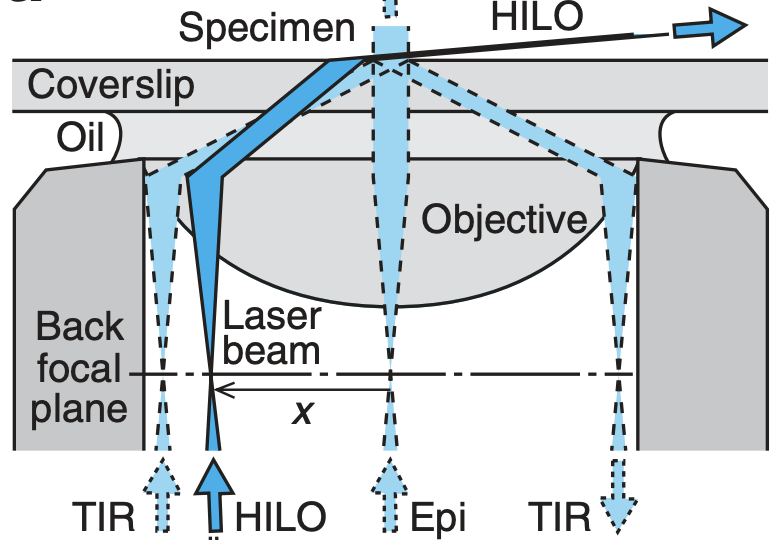
\includegraphics[width=4cm]{../../dissertation/dissertation/media/HILO}
\end{textblock*}

\begin{textblock*}{3cm}(1.5cm,5.75cm)
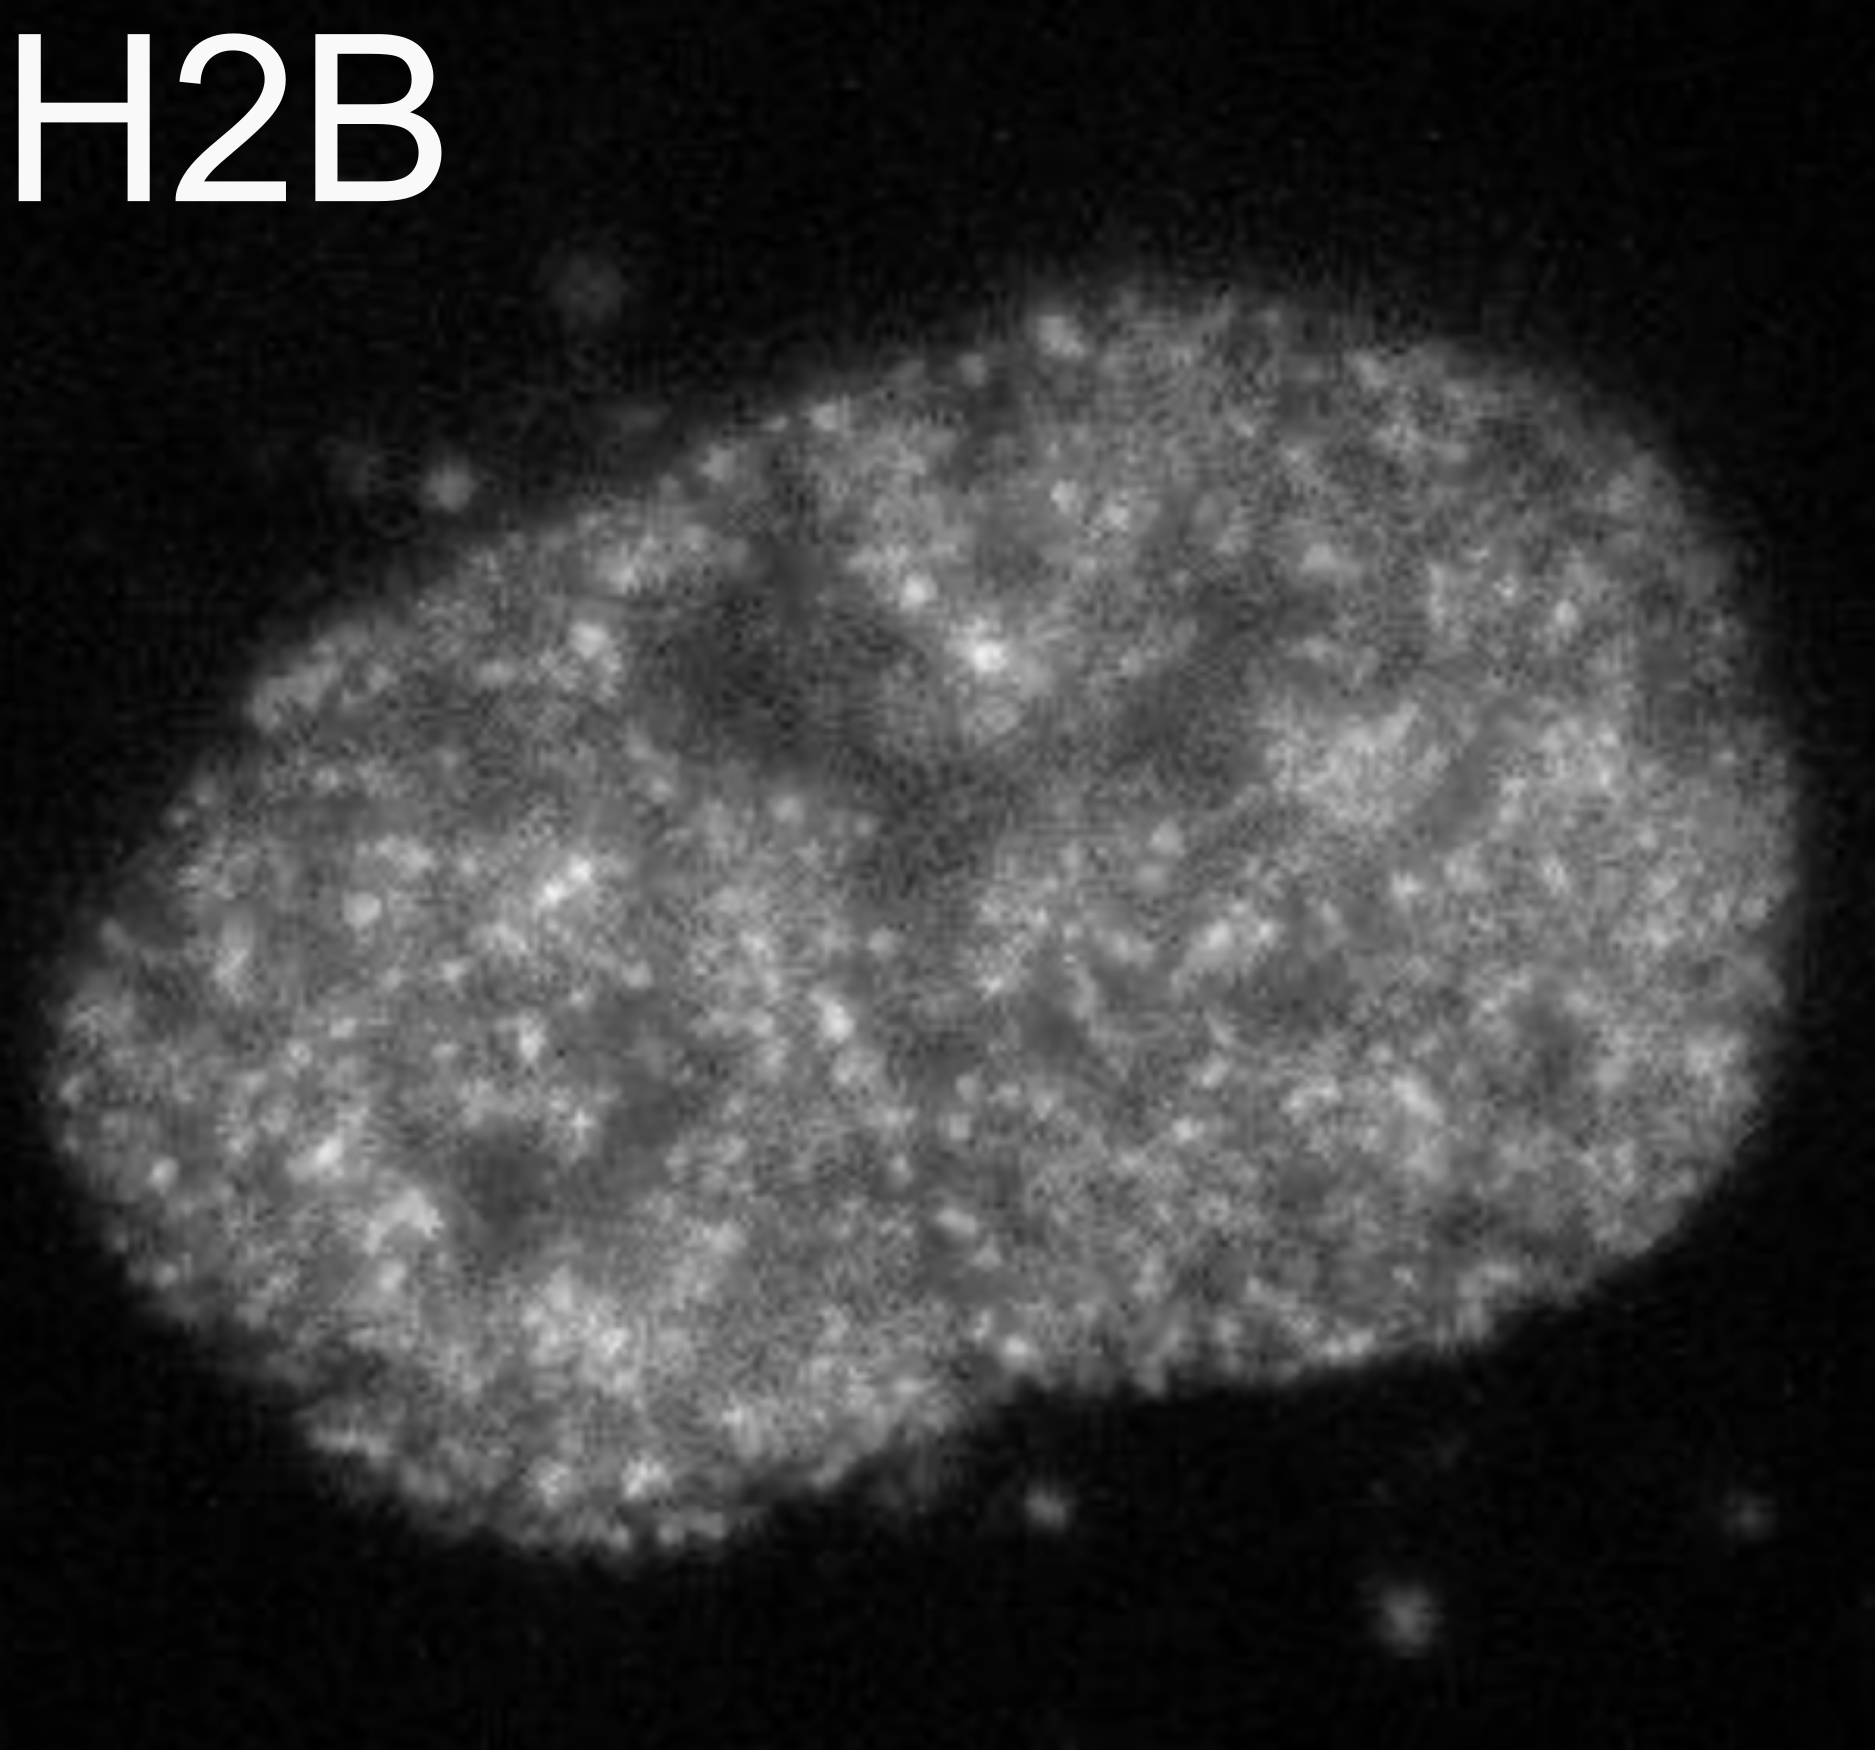
\includegraphics[width=3cm]{../../dissertation/dissertation/media/Widefield}
\end{textblock*}


\begin{textblock*}{8cm}(6.0cm,2.3cm)
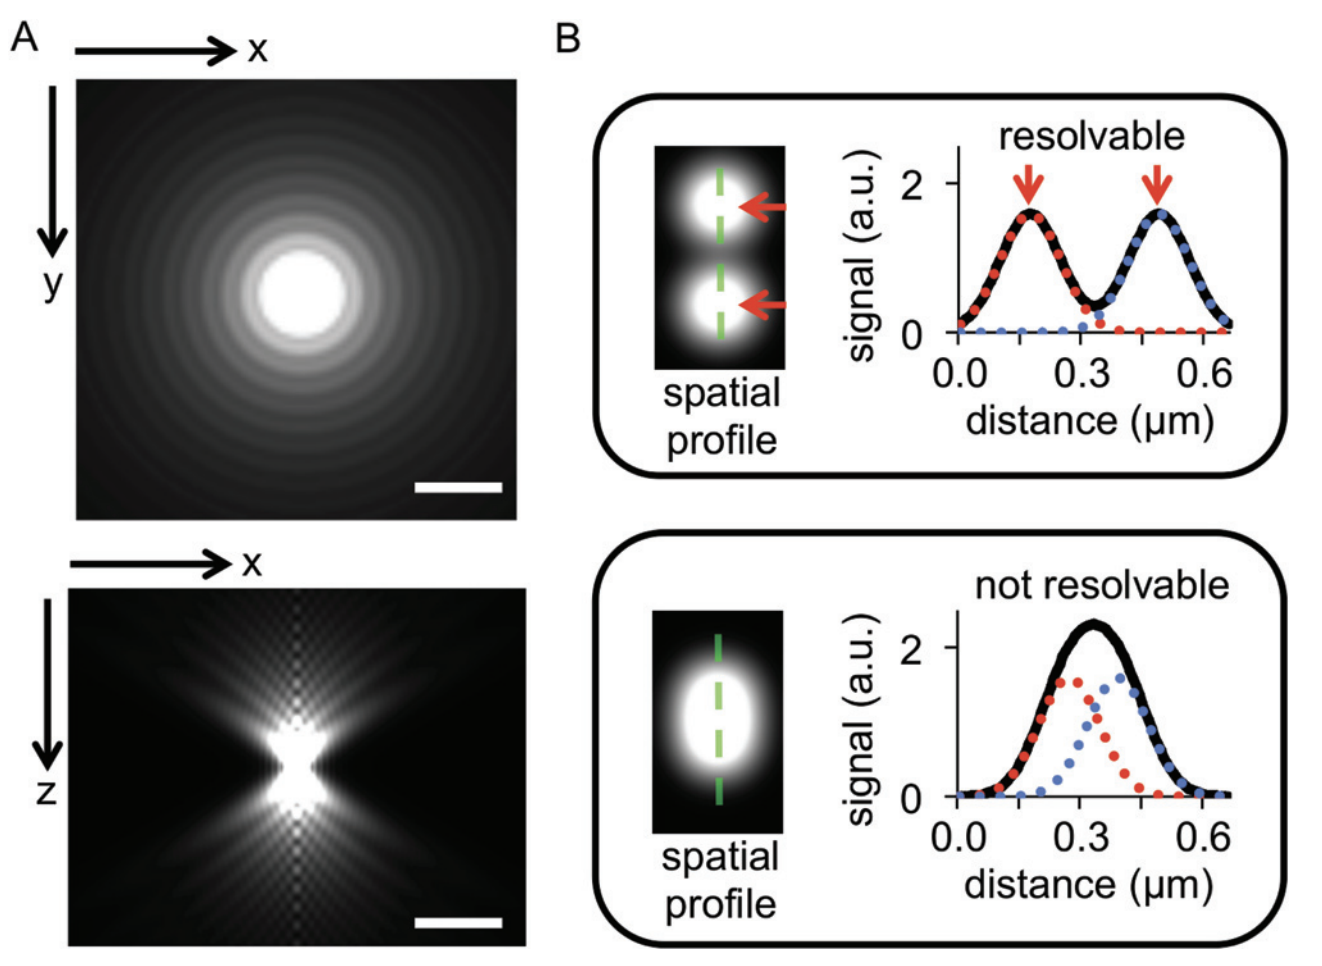
\includegraphics[width=8cm]{../../dissertation/dissertation/media/PSF}
\end{textblock*}

\begin{textblock*}{8cm}(6.3cm,8.3cm)
Herbert et al. Microscopy and Microanalysis.
\end{textblock*}


\end{frame}

\begin{comment}
\begin{frame}{Stochastic optical reconstruction microscopy (STORM)}
\begin{textblock*}{9cm}(0.5cm,1.0cm)
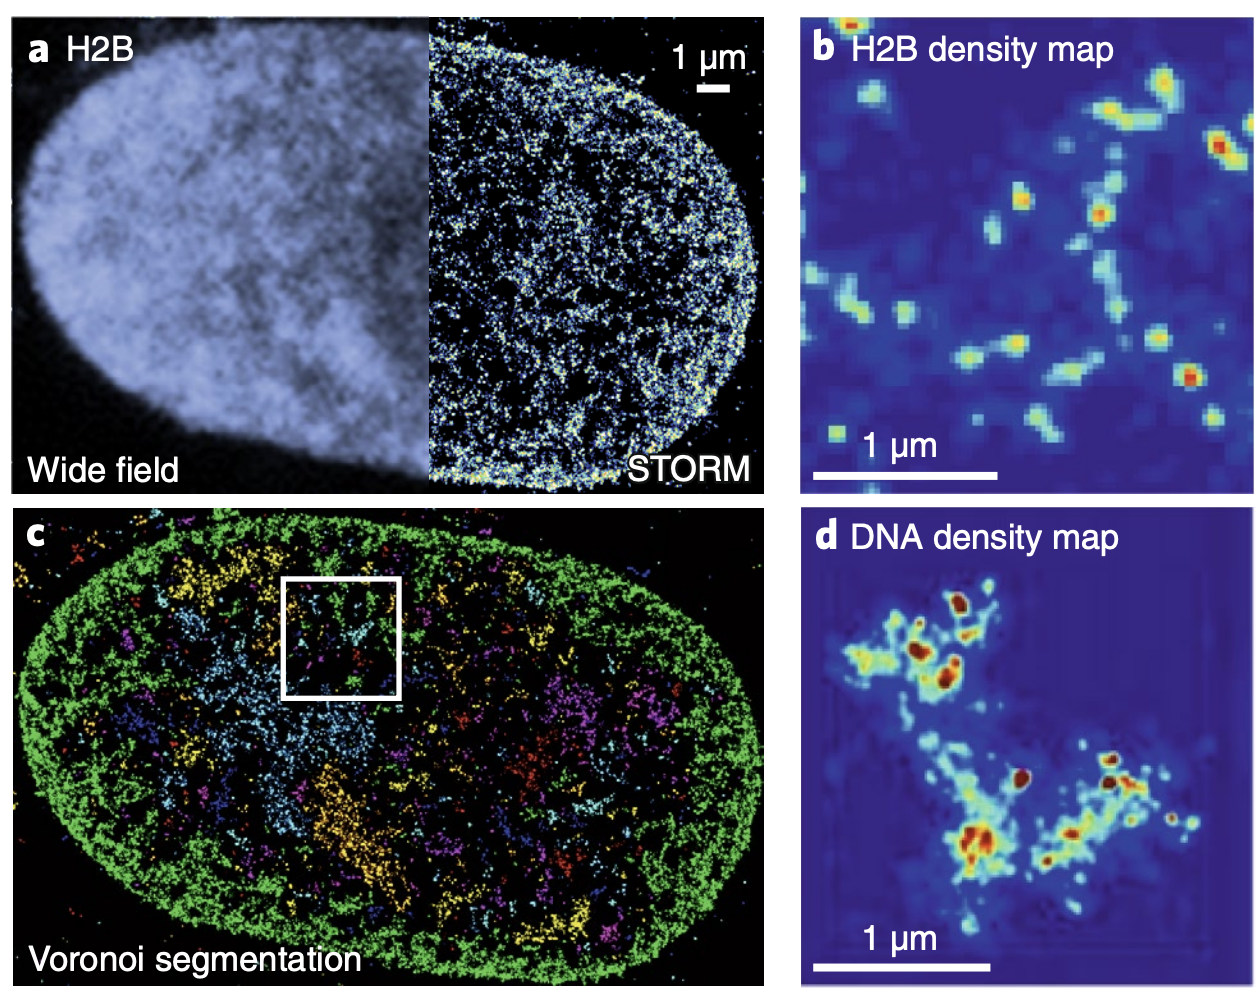
\includegraphics[width=9cm]{../../dissertation/dissertation/media/STORM.png}
Lakadamyali, M. et al. Nature Methods \textbf{17}, (2020).
\end{textblock*}
\begin{textblock*}{3.5cm}(10.0cm,1.1cm)
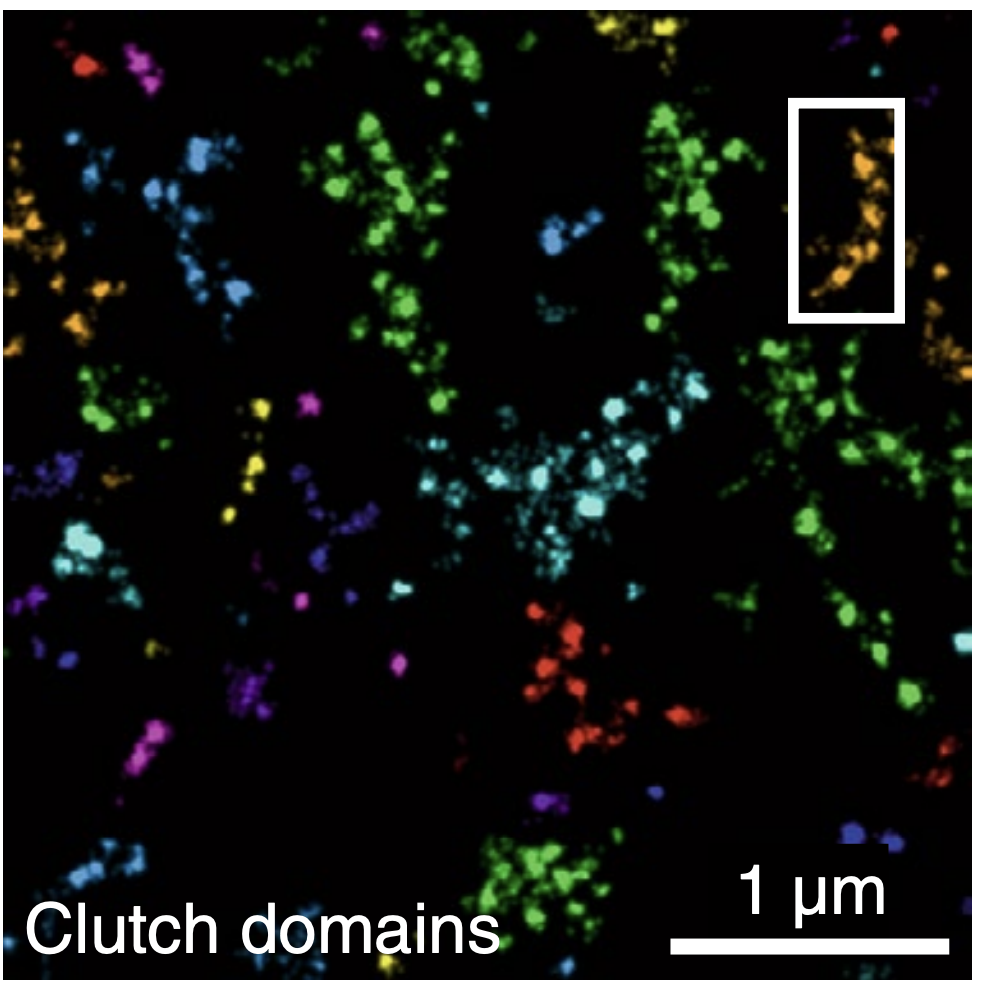
\includegraphics[width=3.5cm]{../../dissertation/dissertation/media/ClutchDomains.png}
\end{textblock*}
\begin{textblock*}{4.5cm}(10.0cm,5.0cm)
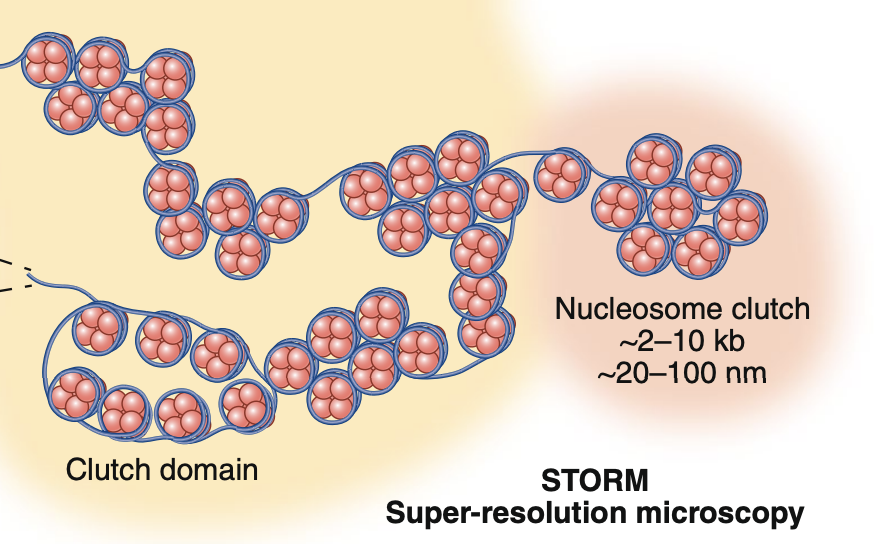
\includegraphics[width=4.5cm]{../../dissertation/dissertation/media/ClutchCartoon.png}
\end{textblock*}
\end{frame}
\end{comment}

\begin{frame}{Stochastic optical reconstruction microscopy (STORM)}
\begin{textblock*}{9cm}(0.5cm,1.5cm)
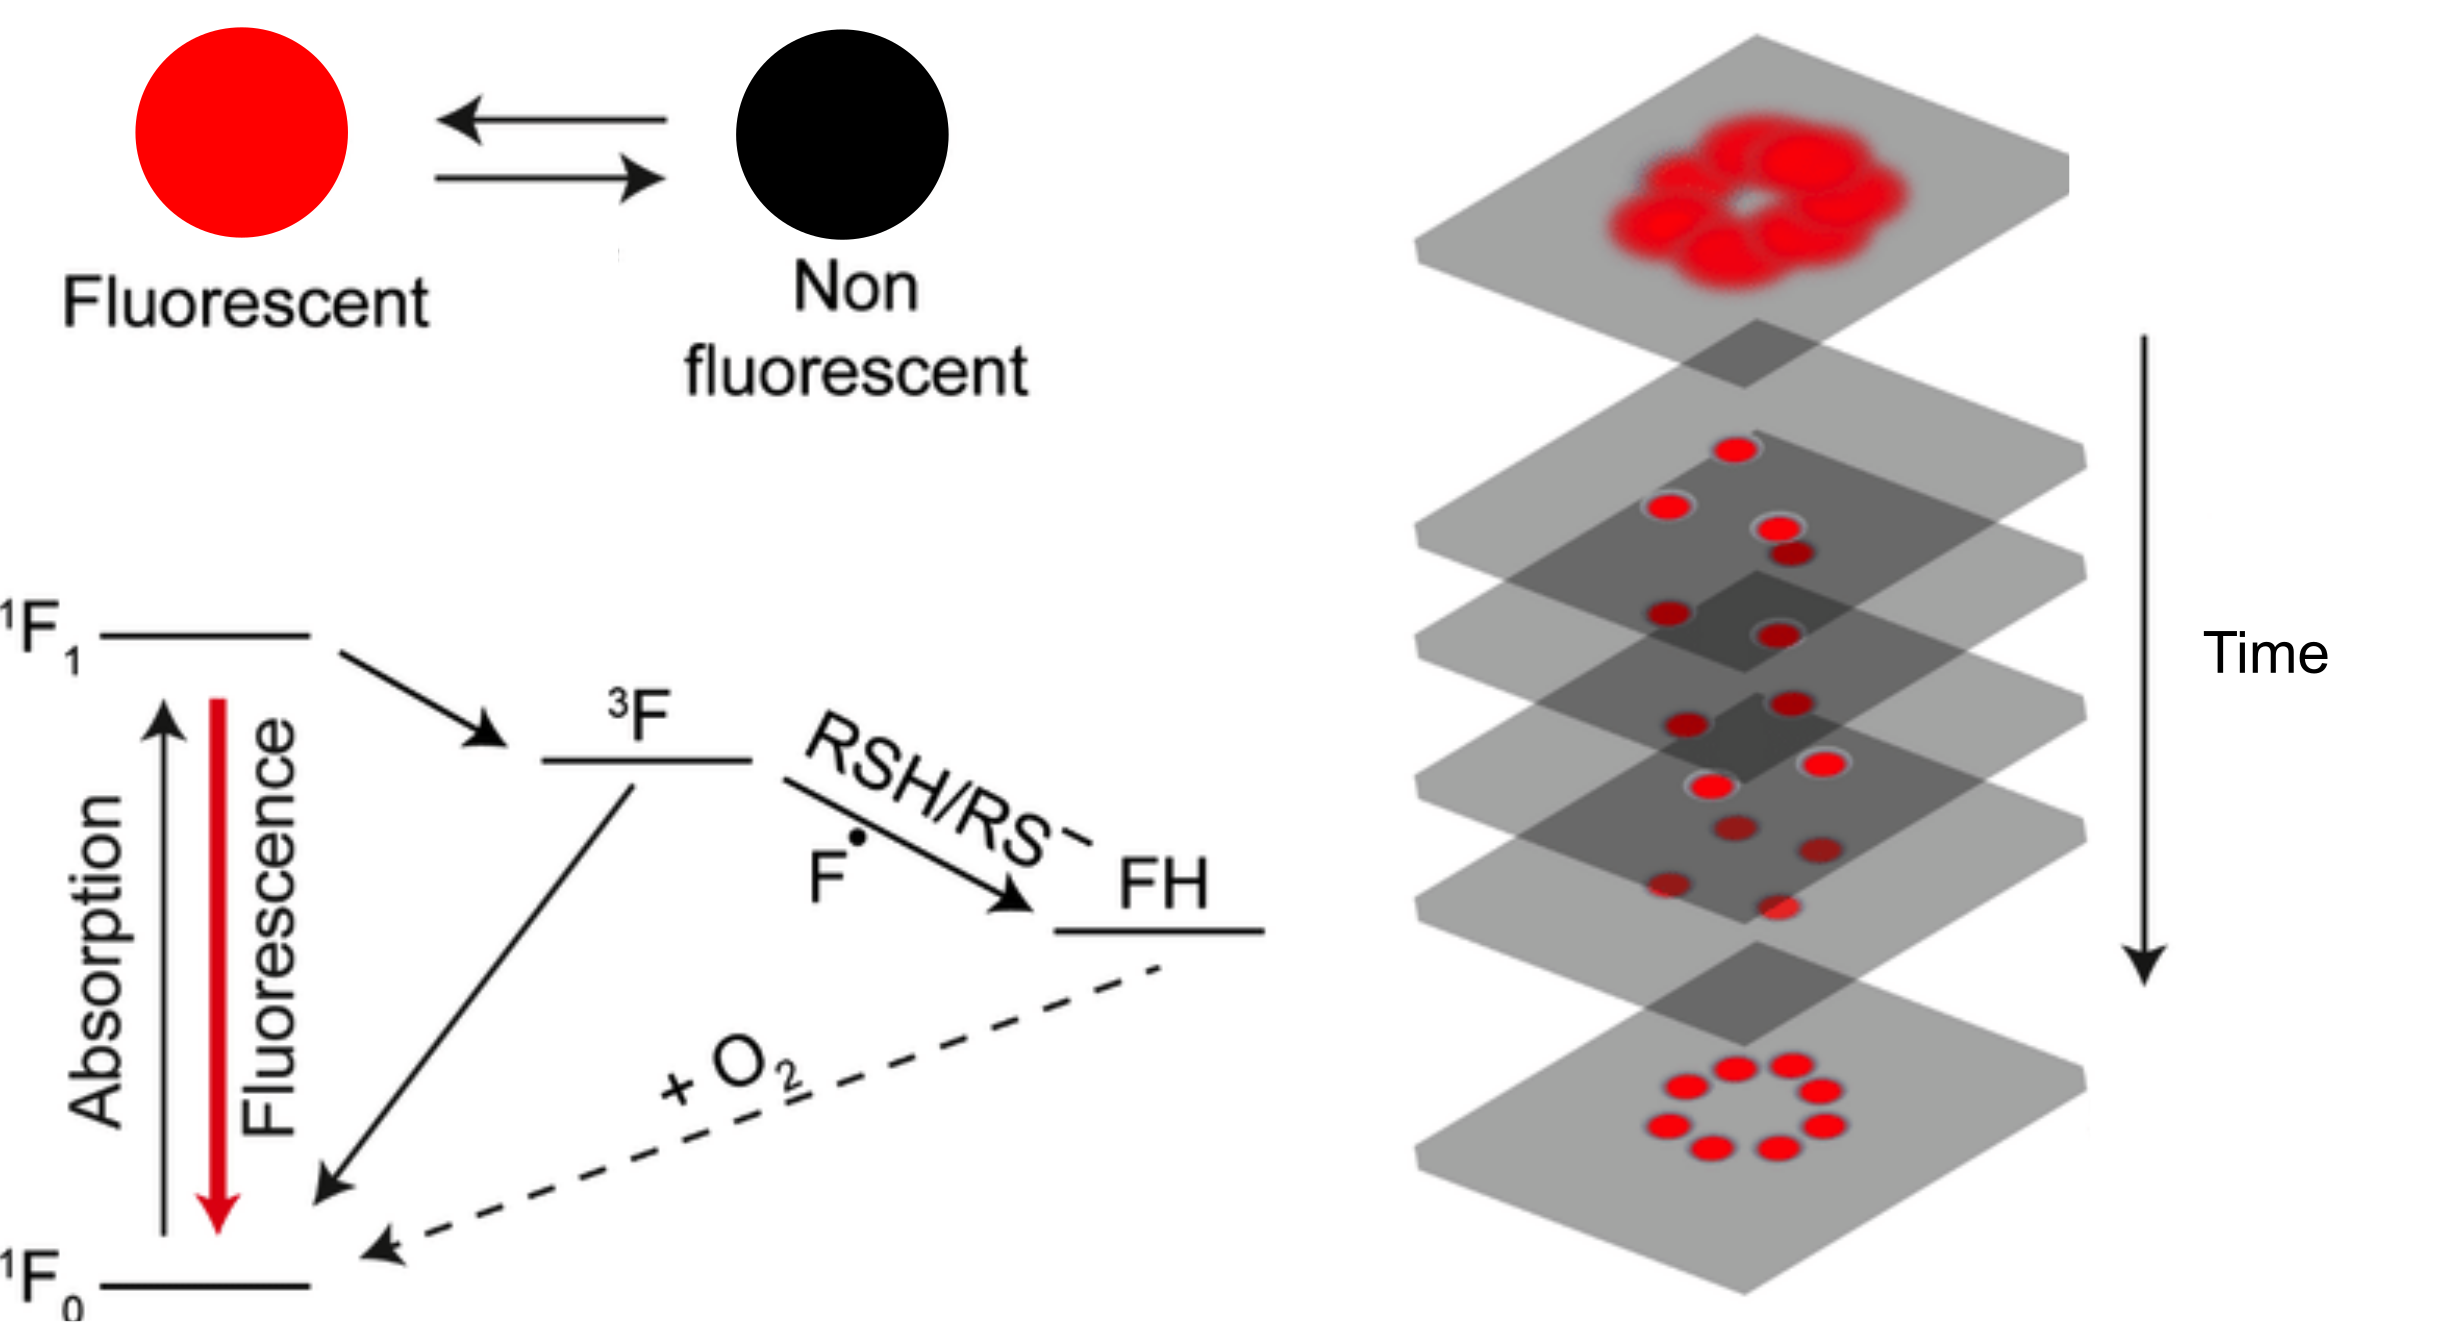
\includegraphics[width=\textwidth]{../../dissertation/dissertation/media/Intro-Cropped.png}
\end{textblock*}
\begin{textblock*}{5cm}(9.5cm,1.5cm)
\animategraphics[width=5cm,autoplay,loop]{60}{../../dissertation/dissertation/media/storm-animation/storm-animation-}{1}{100}
\end{textblock*}
\begin{textblock*}{15cm}(0.5cm,7.5cm)
\begin{itemize}
\item STORM and similar nanoscopy techniques are limited by localization precision
\item Higher lateral/axial resolution than other methods (e.g., SIM,STED,Confocal)
\item Poor time resolution
\end{itemize}
\end{textblock*}
\end{frame}

\begin{frame}{Stochastic optical reconstruction microscopy (STORM)}
\begin{textblock*}{9cm}(0.5cm,1.5cm)
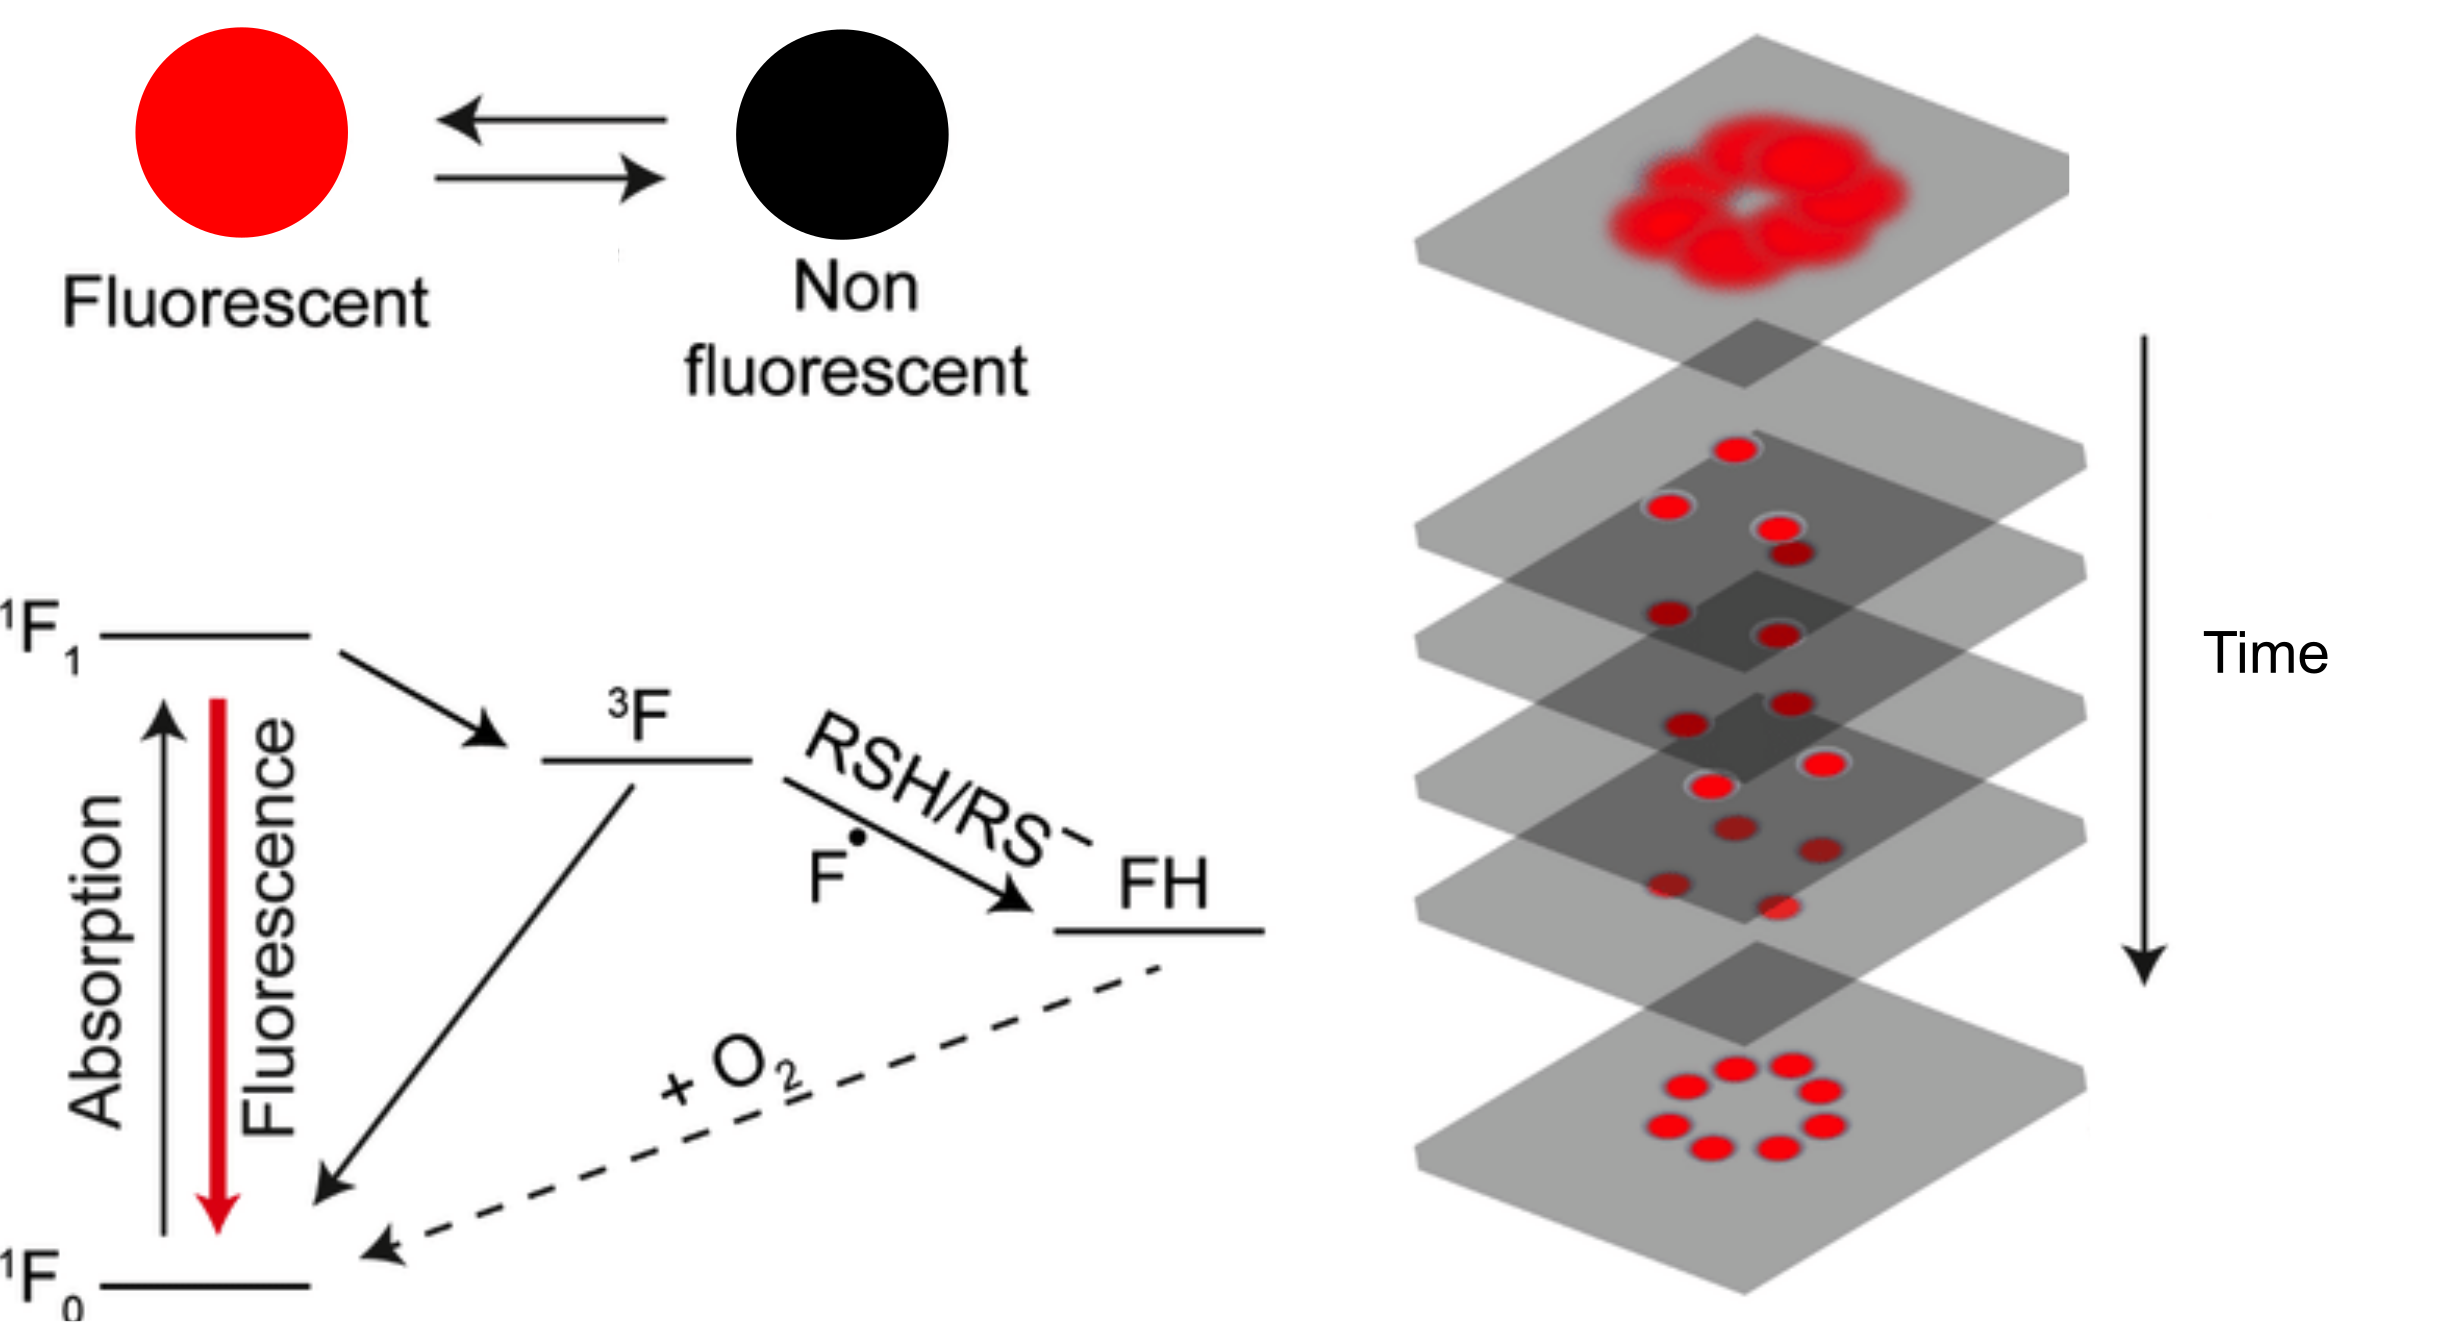
\includegraphics[width=\textwidth]{../../dissertation/dissertation/media/Intro-Cropped.png}
\end{textblock*}
\begin{textblock*}{5cm}(9.5cm,1.5cm)
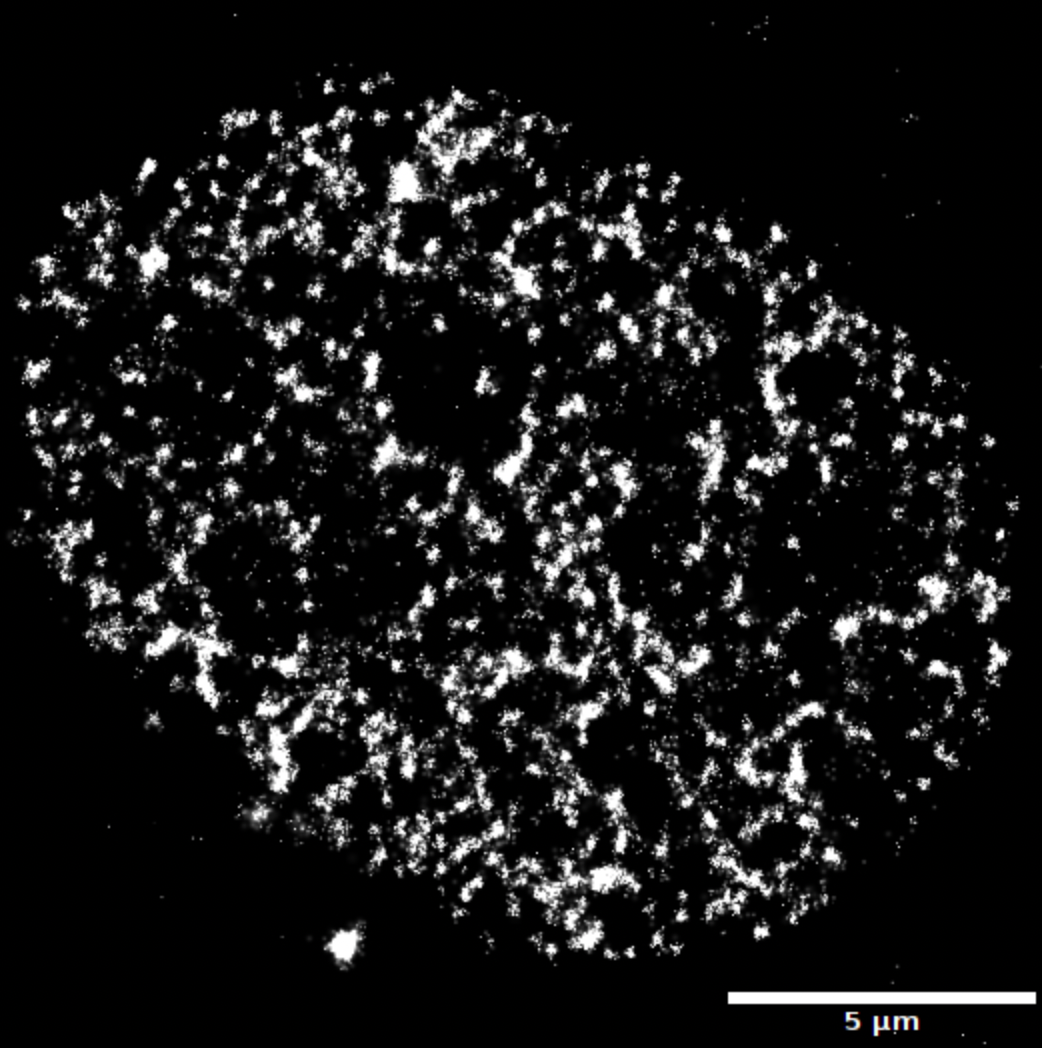
\includegraphics[width=\textwidth]{../../dissertation/dissertation/media/STORM-Example.png}
\end{textblock*}
\begin{textblock*}{15cm}(0.5cm,7.5cm)
\begin{itemize}
\item STORM and similar nanoscopy techniques are limited by localization precision
\item Higher lateral/axial resolution than other methods (e.g., SIM,STED,Confocal)
\item Poor time resolution
\end{itemize}
\end{textblock*}
\end{frame}

%\begin{frame}{Experimental facts of life}
%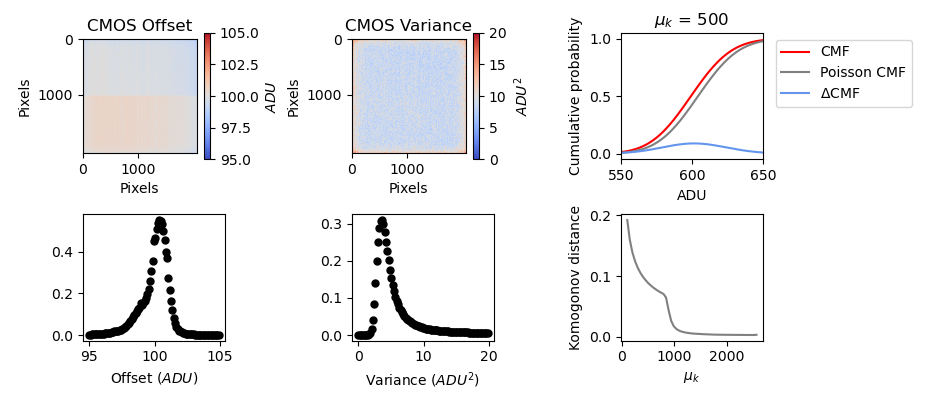
\includegraphics[width=14cm]{../../dissertation/dissertation/media/Noise.png}
%\vspace{0.5in}
%Noise characteristics for air-cooled Hamamatsu ORCA-Flash4.0
%\end{frame}



\begin{frame}{Nanoscopy by localizing isolated fluorescent emitters}
\begin{itemize}
\item Modeling the point spread function permits sub-pixel localization 
\end{itemize}
\begin{textblock*}{8cm}(6.5cm,3.0cm)
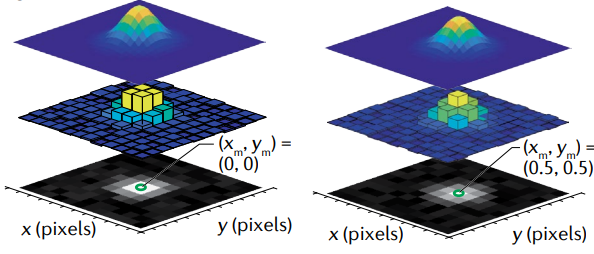
\includegraphics[width=\textwidth]{../../dissertation/dissertation/media/Model.png}
\end{textblock*}

\begin{textblock*}{2cm}(1cm,2.0cm)
\begin{align*}
\mu_{k} &= i_{0}\int\int O(u,v)dudv + \textcolor{pink}{\lambda}\\
i_{0} &= g_{k}\textcolor{red}{\eta} \textcolor{cyan}{\zeta}\textcolor{blue}{\Delta} 
\\
g_{k} &- \mathrm{pixel\; gain}\\
\textcolor{red}{\eta} &- \mathrm{quantum\; efficiency}\\
\textcolor{cyan}{\zeta} &- \mathrm{photon\; emission\; rate}\\
\textcolor{blue}{\Delta} &- \mathrm{exposure\; time}\\
\textcolor{pink}{\lambda} &- \mathrm{background \; rate}
\end{align*}
\end{textblock*}

\vspace{2in}

Maximum likelihood localization:

\begin{equation*}
\theta^{*} = \underset{\theta}{\mathrm{argmax}}\prod_{k}p(\bold{x}_{k}|\theta)= \underset{\theta}{\mathrm{argmin}}-\sum_{k}\log p(\bold{x}_{k}|\theta)
\end{equation*}

\end{frame}

\begin{frame}{Applications of single molecule localization microscopy}
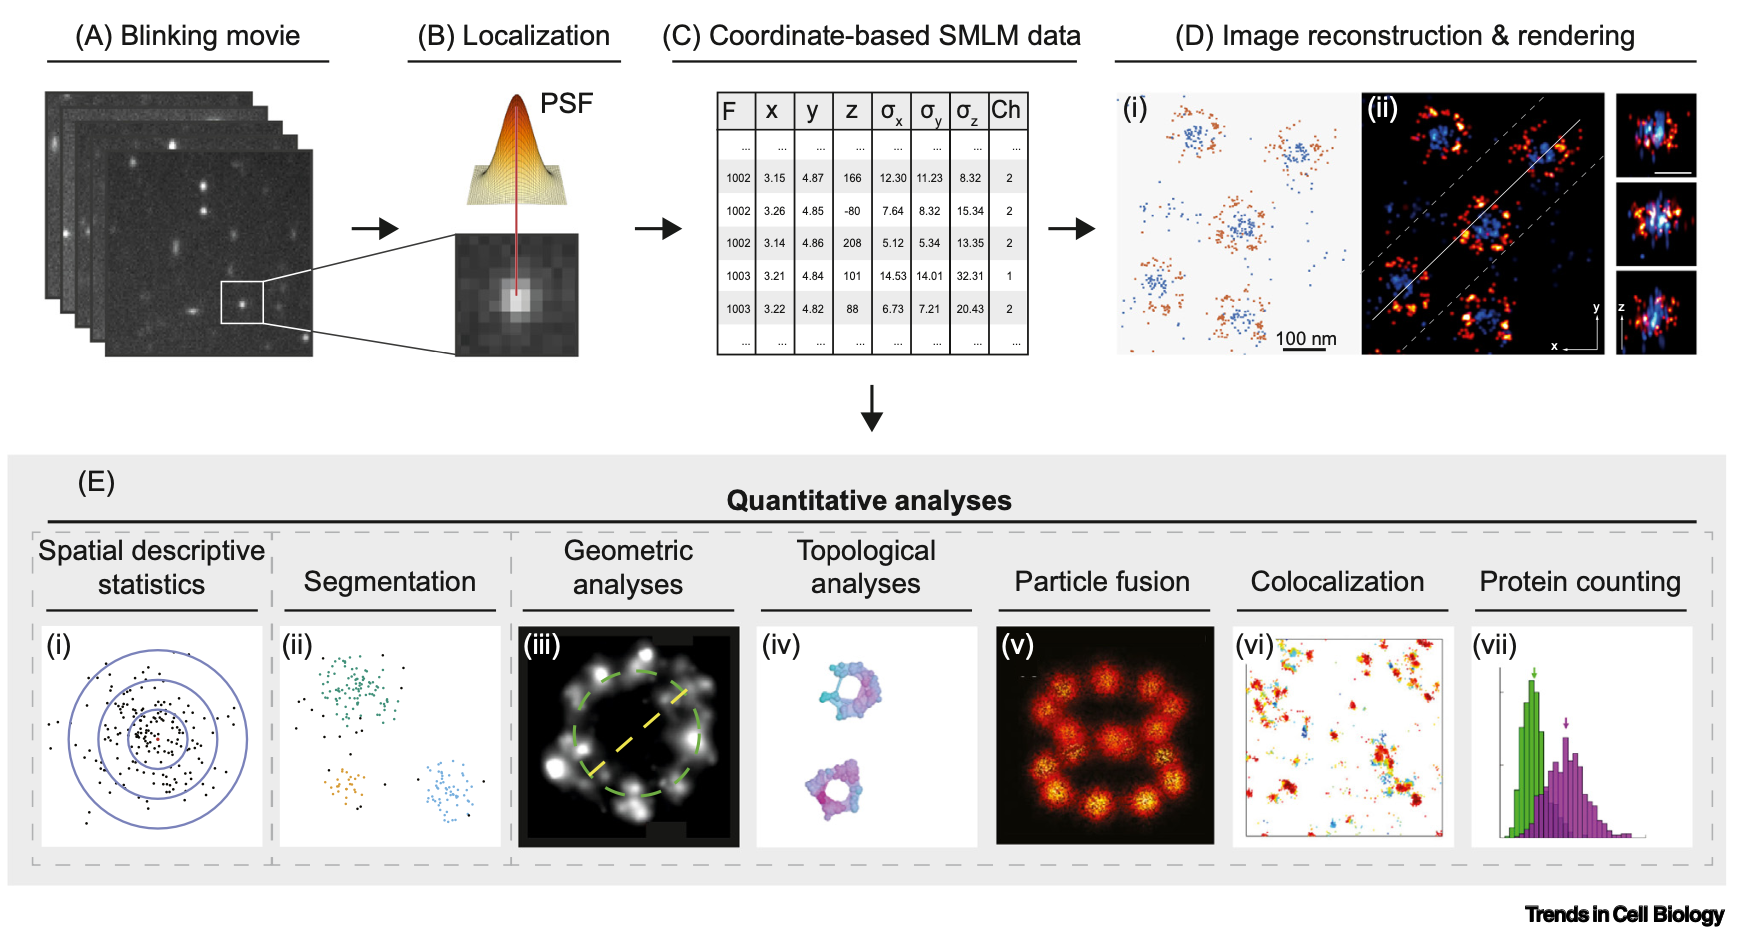
\includegraphics[width=\textwidth]{../../dissertation/dissertation/media/Apps.png}
Wu et al. Trends in Cell Biology. \textbf{30} (2020)
\end{frame}


\begin{comment}
\begin{frame}
\frametitle{Super resolution with photoswitching of rhodamines}

\begin{figure}
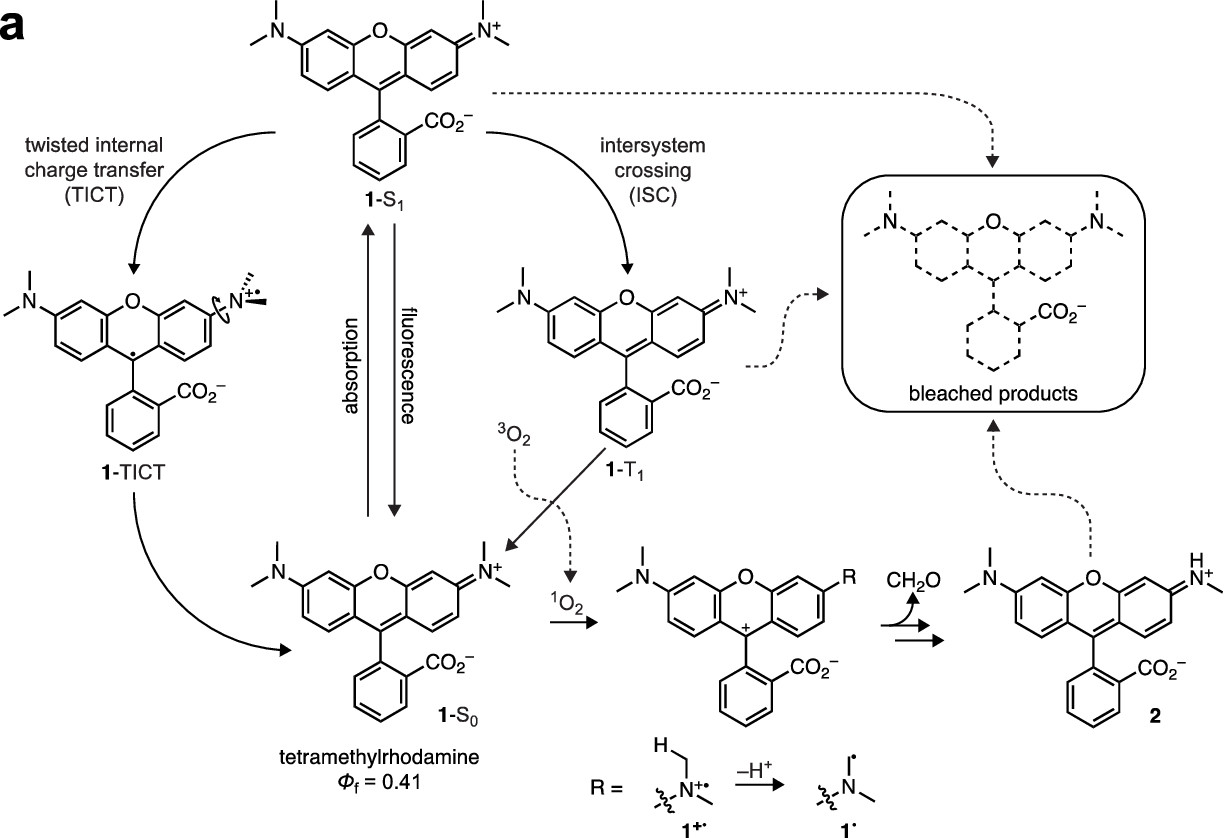
\includegraphics[width=10cm]{../../dissertation/dissertation/media/Rhodamines.png}
\end{figure}
\begin{itemize}
\item  Reduction of the T1 state yields a dark, long-lived, and stable radical state
\end{itemize}
\end{frame}
\end{comment}

\begin{comment}
\begin{frame}
\frametitle{Direct stochastic optical reconstruction microscopy}

\begin{figure}
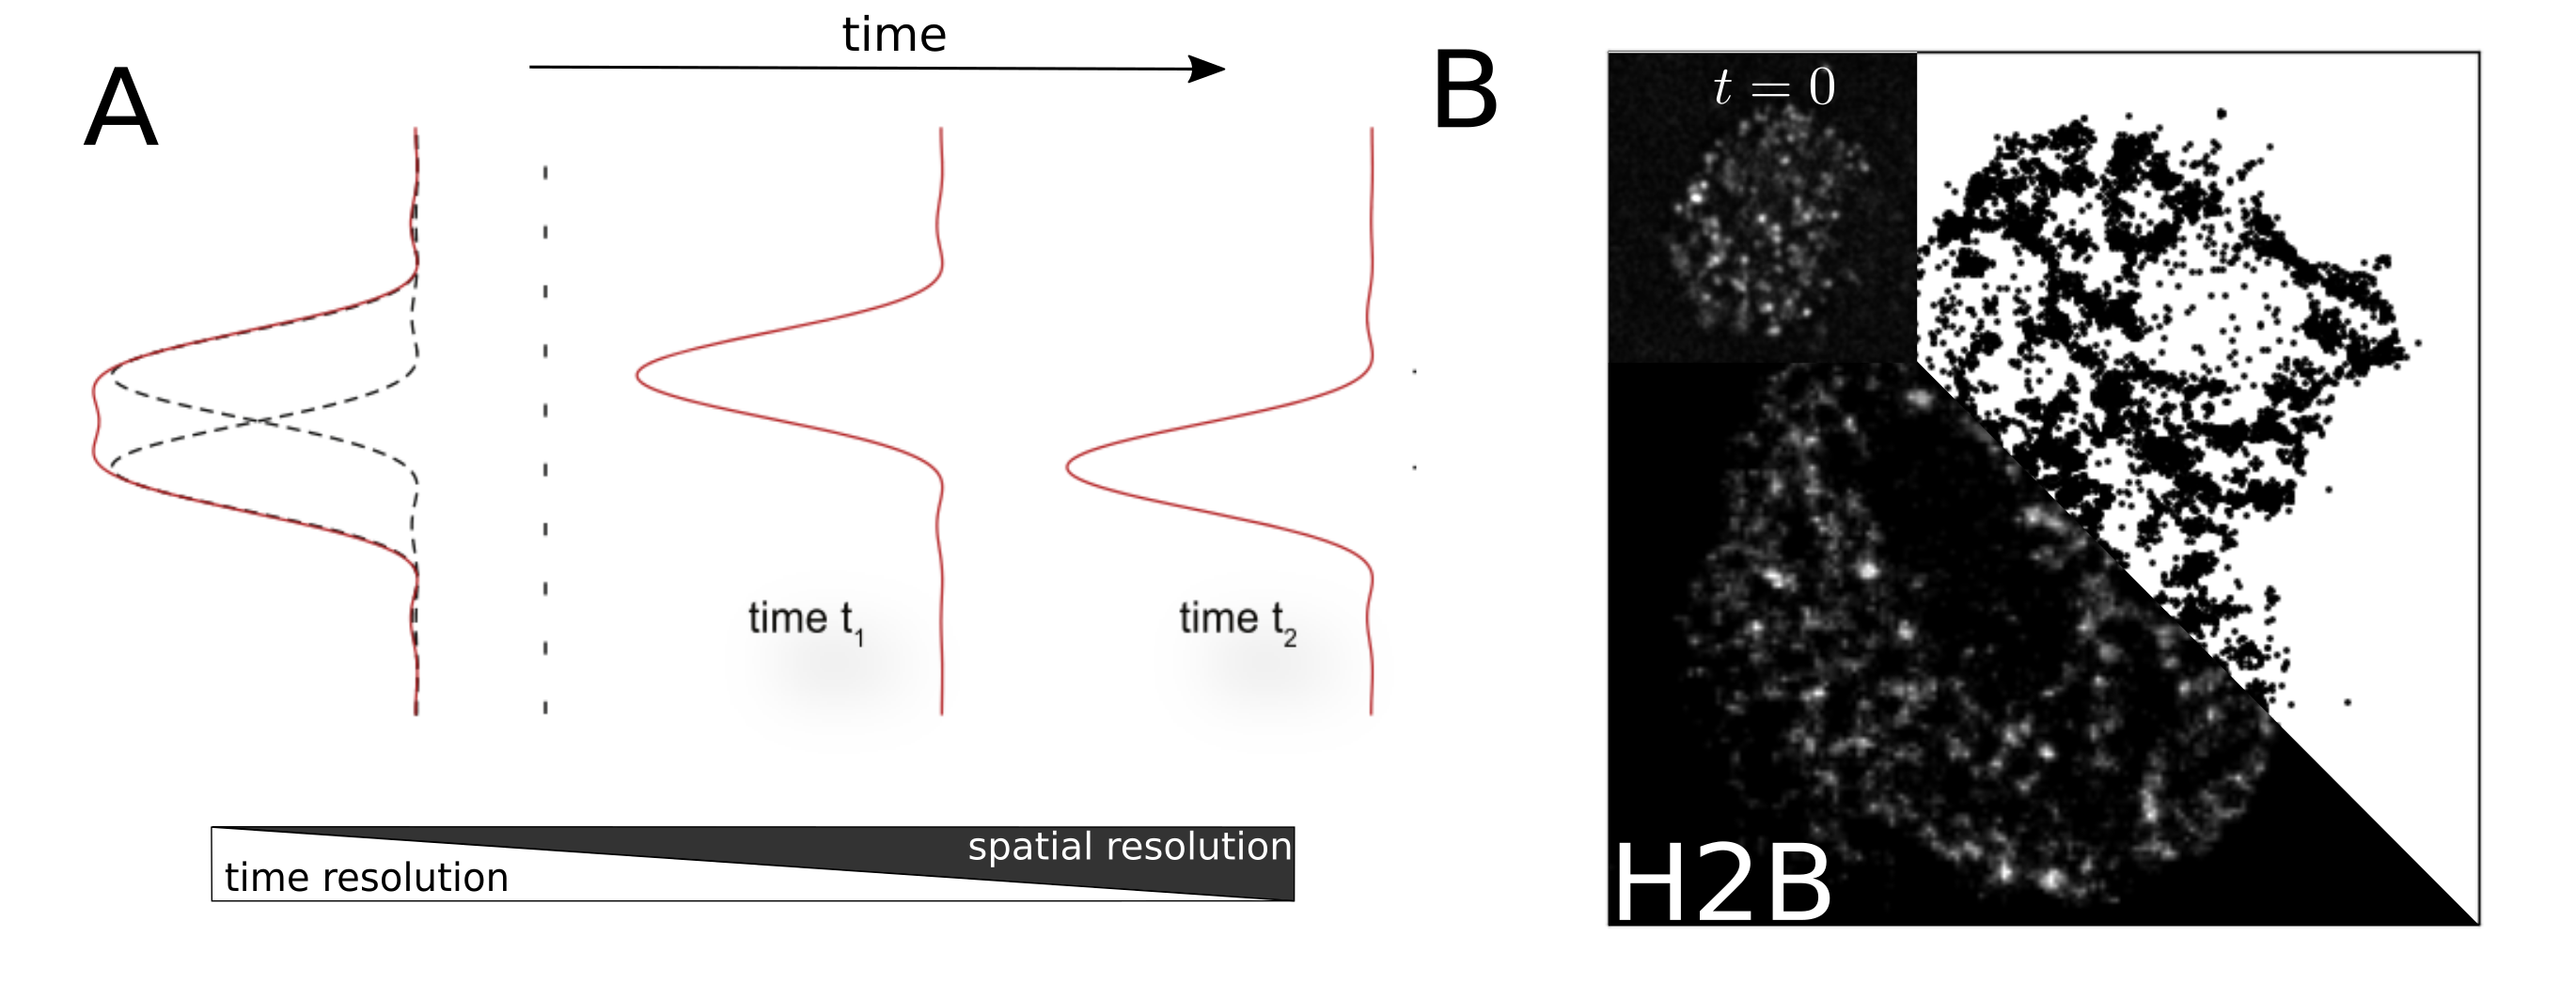
\includegraphics[width=13cm]{../../dissertation/dissertation/media/Concept.png}
\end{figure}

\begin{itemize}
\item Photoswitching enables resolution of emitters in time rather than space
\item Presents a tradeoff between spatial and temporal resolution
\end{itemize}

\end{frame}
\end{comment}

\begin{frame}
\frametitle{Maximization of density, minimization of error}

\begin{textblock*}{8cm}(0.5cm, 1.5cm)
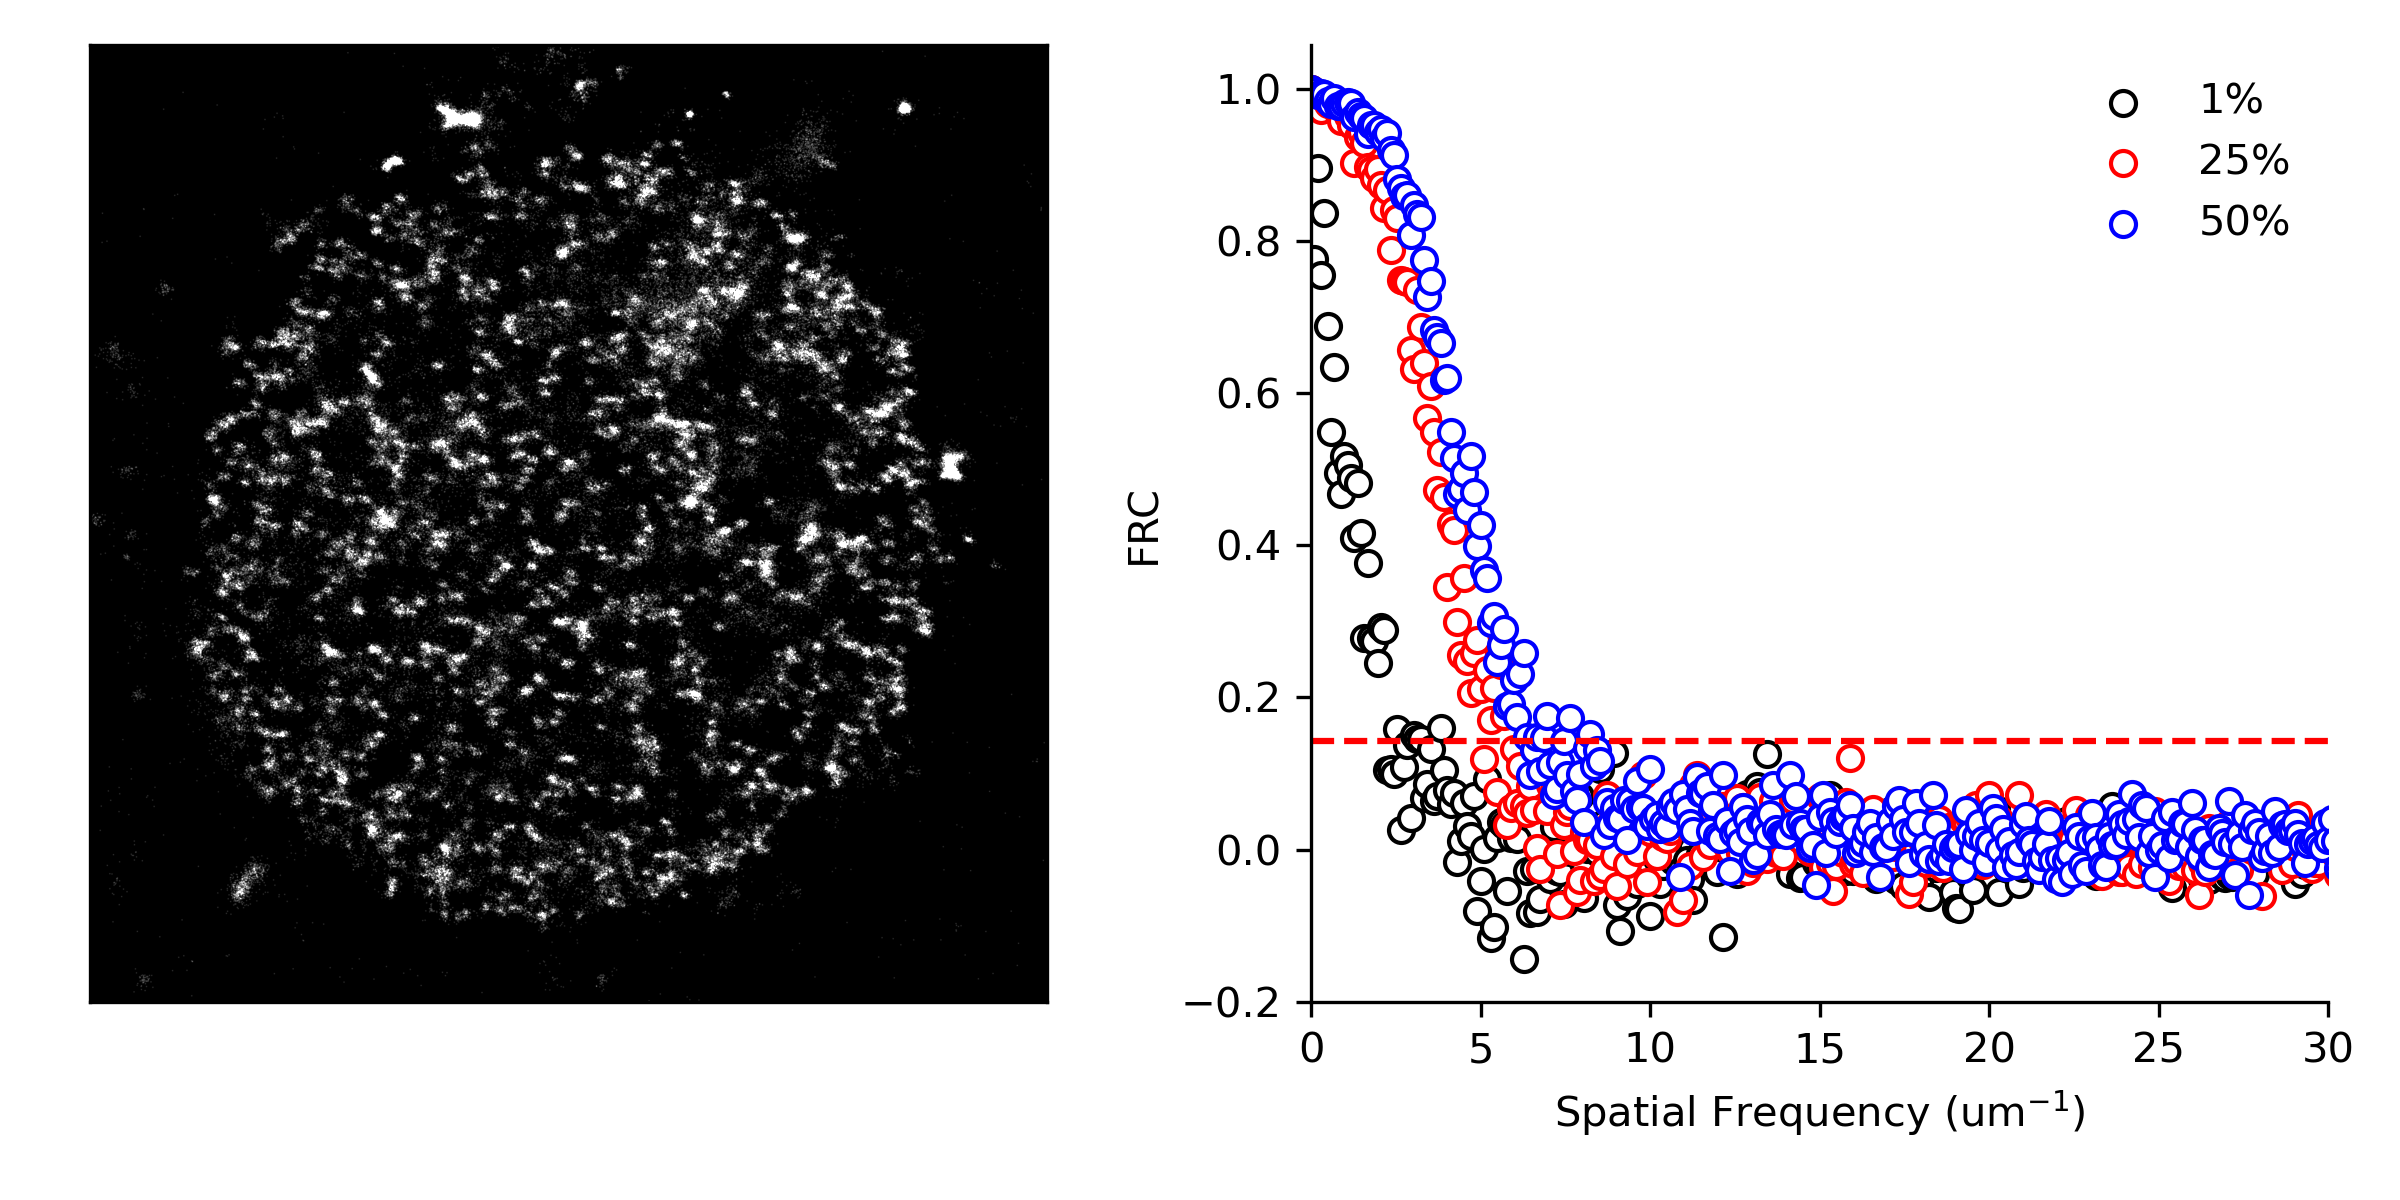
\includegraphics[width=8cm]{../../dissertation/dissertation/media/FRC.png}
\end{textblock*}

\begin{textblock*}{5cm}(9.35cm, 1.75cm)
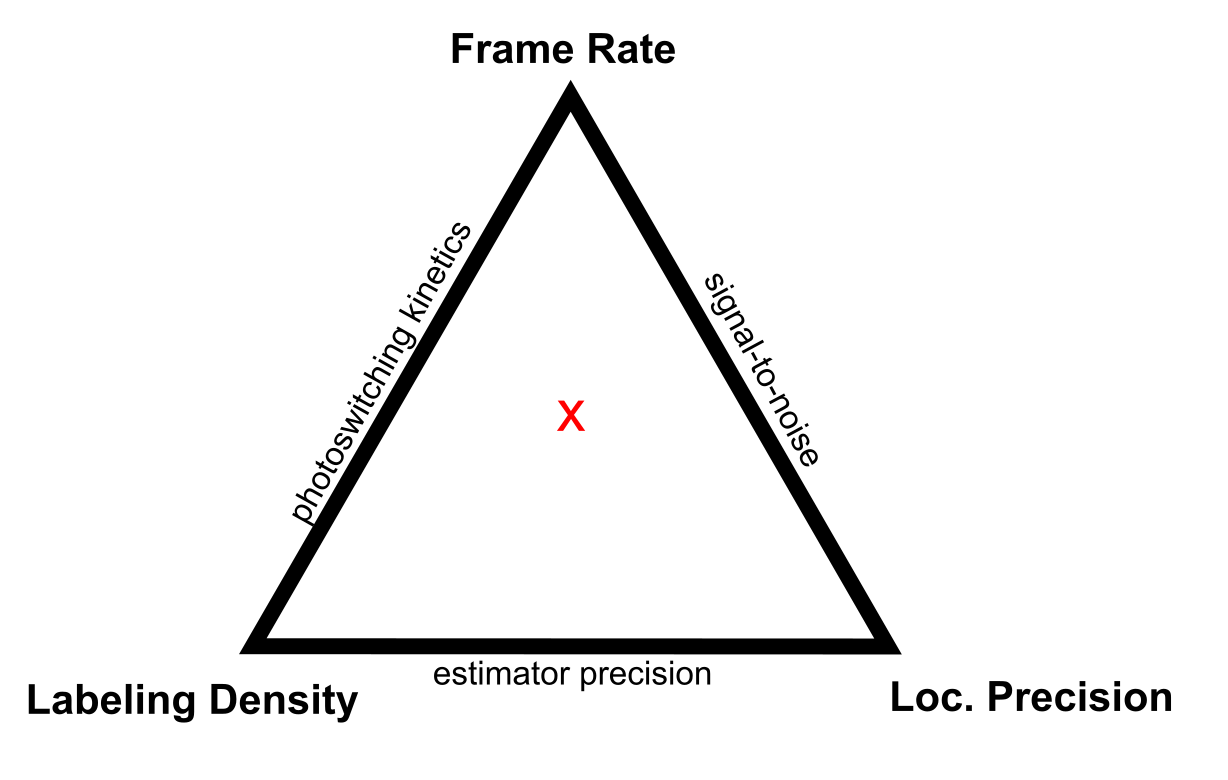
\includegraphics[width=5cm]{../../dissertation/dissertation/media/Tradeoff.png}
\end{textblock*}


\begin{textblock*}{6cm}(8.5cm, 6.0cm)
\begin{itemize}
\item Maximize density and in turn spatial/temporal resolution
\item Minimize localization errors 
\end{itemize}
\end{textblock*}

\end{frame}

\begin{frame}
\frametitle{Maximization of density, minimization of error}

\begin{textblock*}{8cm}(0.5cm, 1.5cm)
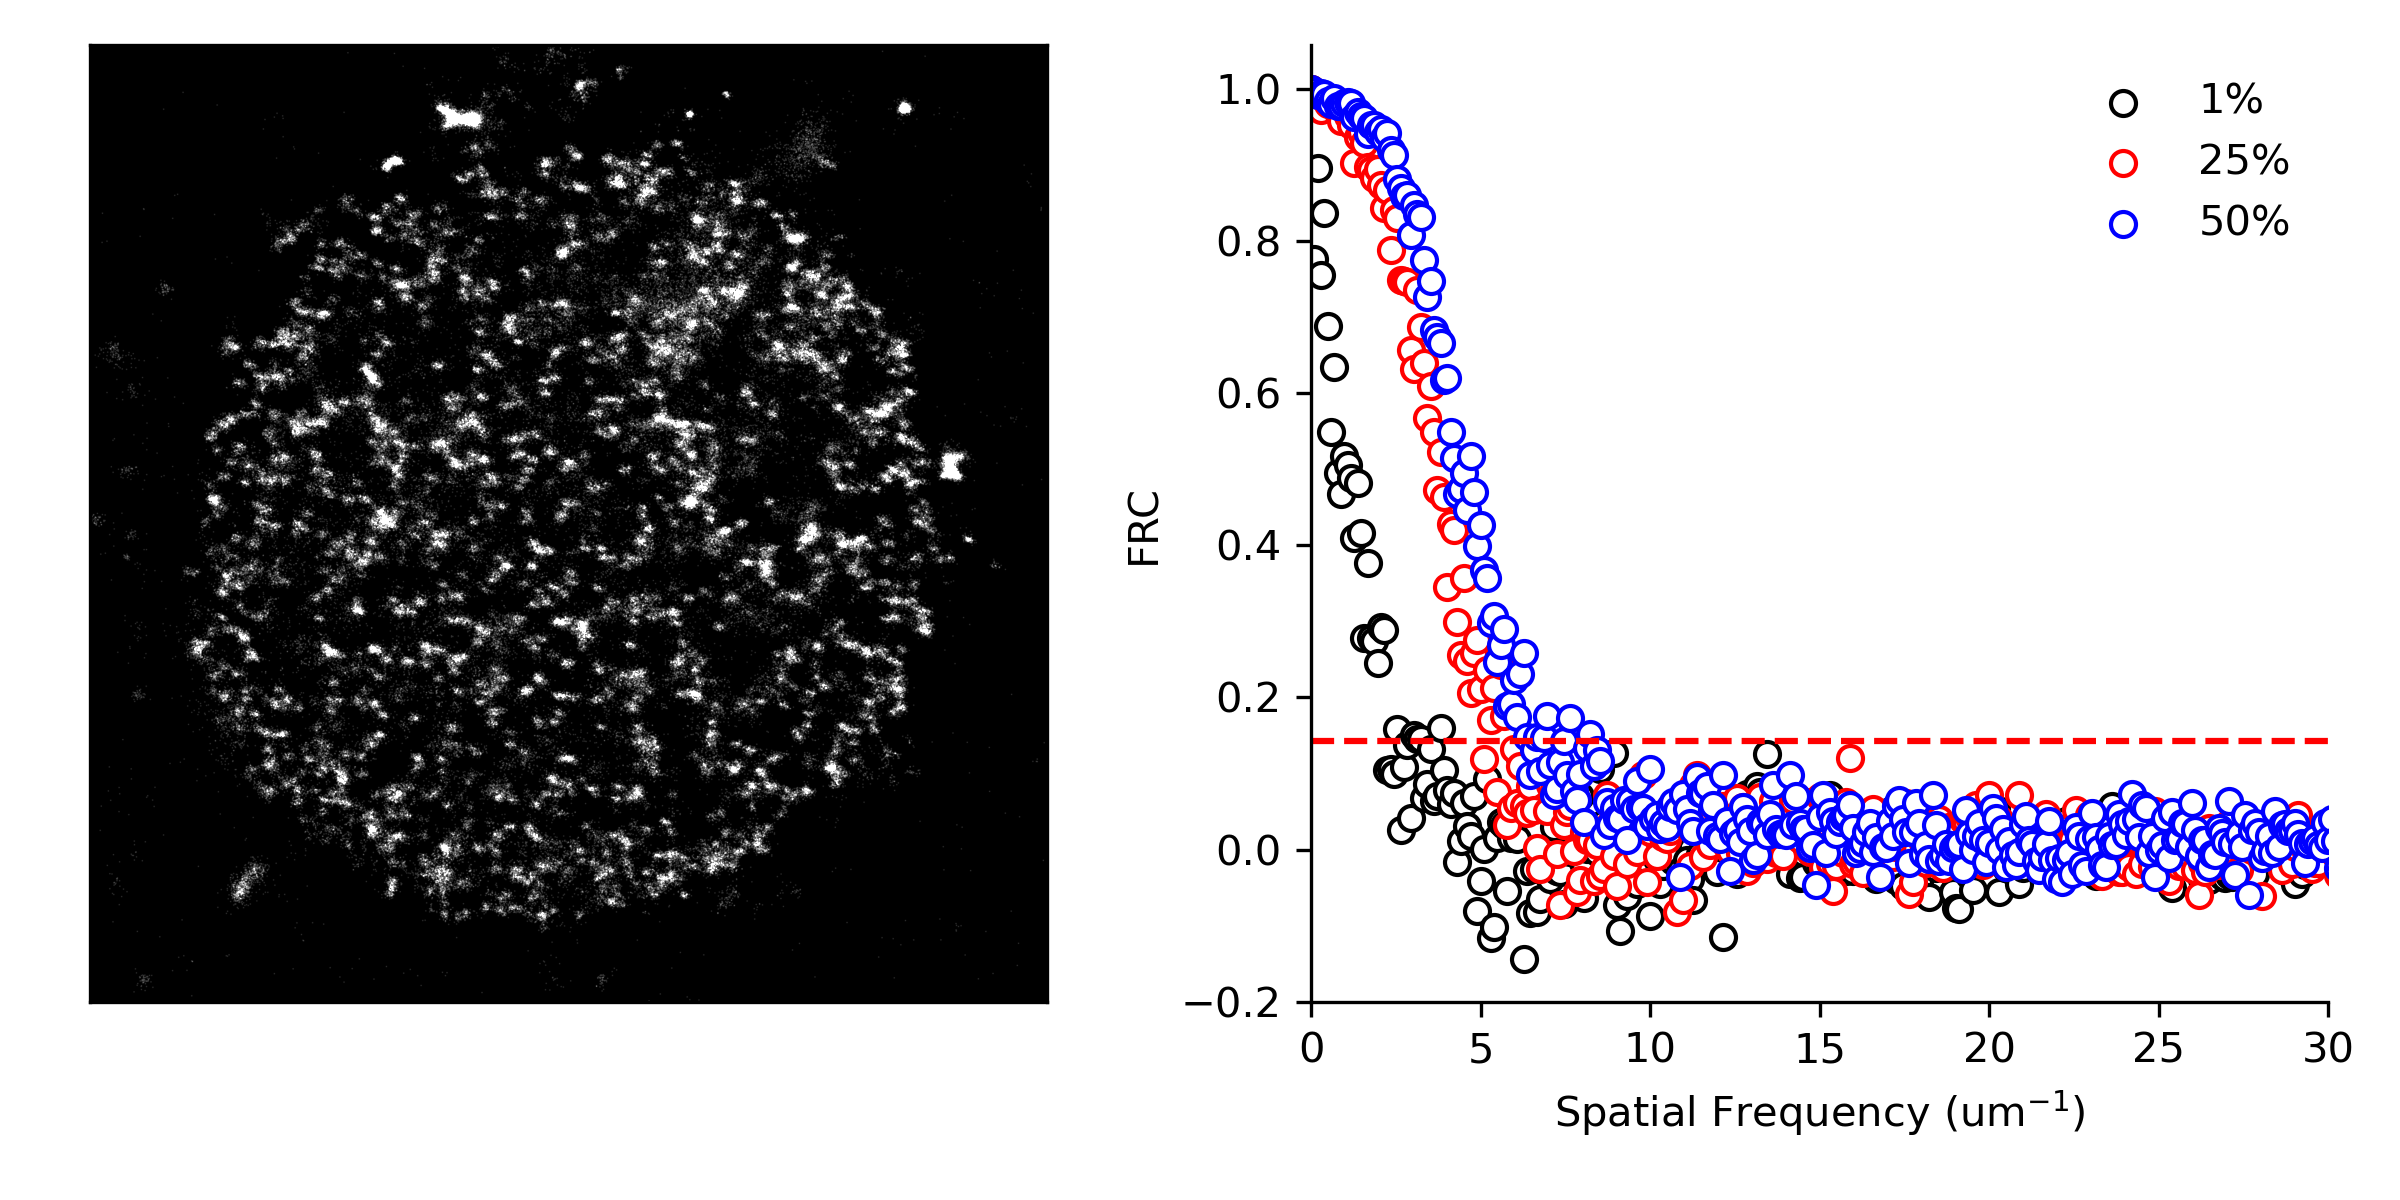
\includegraphics[width=8cm]{../../dissertation/dissertation/media/FRC.png}
\end{textblock*}

\begin{textblock*}{5cm}(9.35cm, 1.75cm)
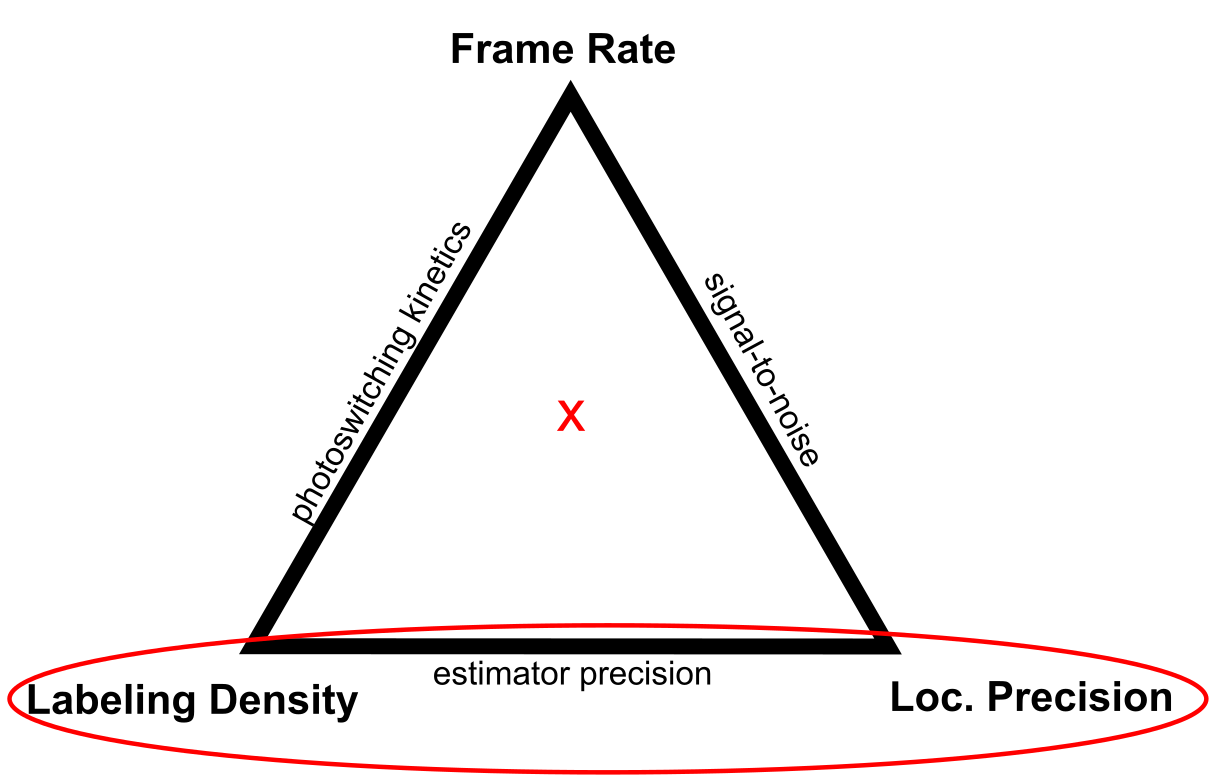
\includegraphics[width=5cm]{../../dissertation/dissertation/media/Tradeoff2.png}
\end{textblock*}


\begin{textblock*}{6cm}(8.5cm, 6.0cm)
\begin{itemize}
\item Maximize density and in turn spatial/temporal resolution
\item Minimize localization errors 
\end{itemize}
\end{textblock*}

\end{frame}

\begin{comment}
\begin{frame}
\frametitle{Maximization of density, minimization of error}

Approach these objectives using two probabilistic modeling approaches:
\begin{itemize}
\item \textbf{Approach I}: Utilize deep generative modeling for \emph{dense} widefield nanoscopy
\item \textbf{Approach II}: Introduce single photon counting in widefield nanoscopy
\end{itemize}

\end{frame}
\end{comment}

%\begin{frame}
%\frametitle{Fourier Image Resolution (FIRE)}

%\begin{figure}
%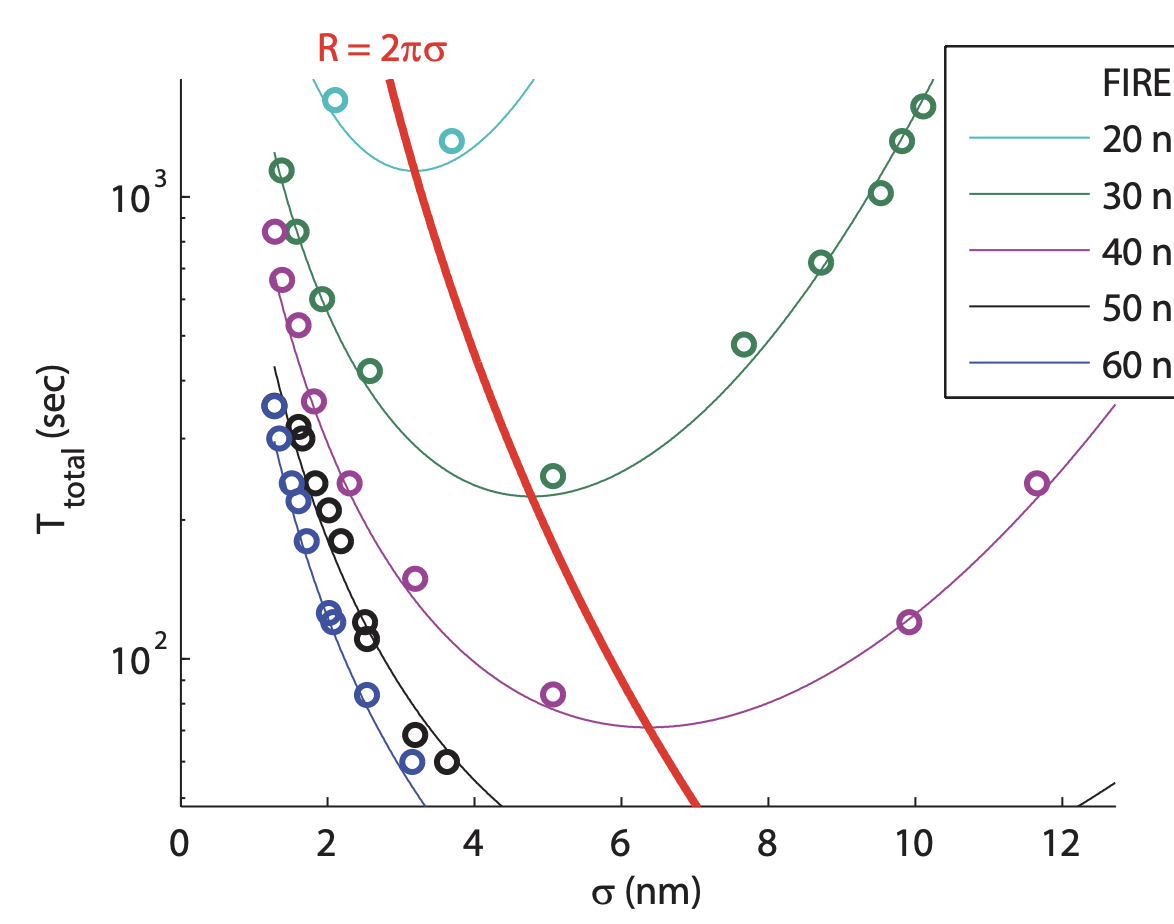
\includegraphics[width=8cm]{../../dissertation/dissertation/media/FIRE.png}
%\end{figure}
%Nieuwenhuizen et al. Nature Methods. \textbf{10} (2013)\\
%\vspace{0.2in}
%Nutshell: \emph{How to relax the density limit in localization microscopy}?
%\end{frame}

\setbeamertemplate{footline}{
    \hbox{%
    \begin{beamercolorbox}[wd=\paperwidth,ht=1.0ex,dp=1.5ex,leftskip=2ex,rightskip=2ex]{page ooter}%
        \footnotesize
        \usebeamerfont{title in head/foot}%
        Novel methods: probabilistic modeling approaches to fluorescence nanoscopy \hfill
            %\insertsection \hfill
        \insertframenumber{} / \inserttotalframenumber
    \end{beamercolorbox}}%
}

\section{Novel methods: Probabilistic modeling approaches to fluorescence nanoscopy}


\subsection{Approach I: Enhance nanoscopy with deep generative models}

\begin{frame}{The Bayesian calculation and variational inference}

%Let $\theta$ be a latent variable (e.g. high resolution image) to be inferred from a measurement $\bold{x}$ (e.g. low resolution image)\\

\textbf{Bayes Rule:}\;\;$p(\theta\lvert \boldsymbol{x}) = \frac{p(\boldsymbol{x}\lvert \theta)p(\theta)}{\int p(\bold{x},\theta)d\theta} \propto p(\boldsymbol{x}\lvert \theta)p(\theta)$
\vspace{0.75cm}

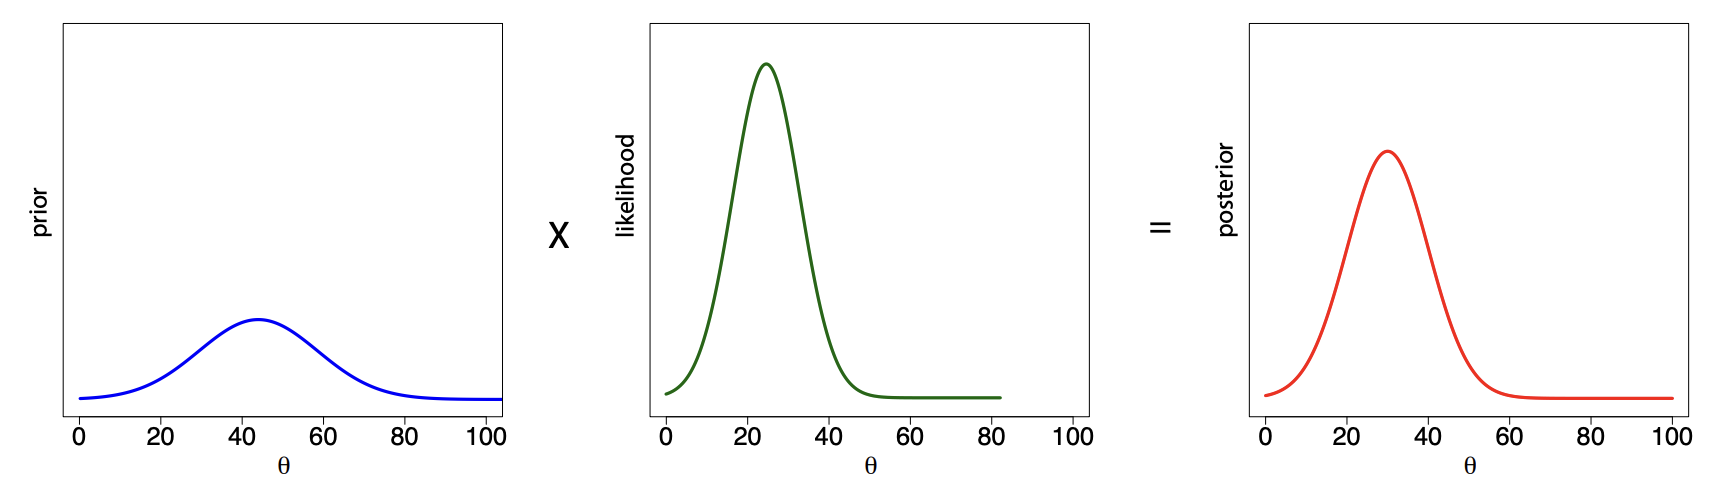
\includegraphics[width=12cm]{../../dissertation/dissertation/media/BayesRule.png}
\vspace{0.5cm}

\begin{itemize}
\item The posterior $p(\theta\lvert \boldsymbol{x})$ is can be hard to obtain
\item Variational inference: fit a model distribution $p_{\psi}(\theta\lvert \boldsymbol{x})$ with parameters $\psi$
\item Can naturally represent uncertainty during inference
\end{itemize}

\end{frame}


\setbeamertemplate{footline}{
    \hbox{%
    \begin{beamercolorbox}[wd=\paperwidth,ht=1.0ex,dp=1.5ex,leftskip=2ex,rightskip=2ex]{page ooter}%
        \footnotesize
        \usebeamerfont{title in head/foot}%
        Figure credit: Roy Friedman \hfill
            %\insertsection \hfill
        \insertframenumber{} / \inserttotalframenumber
    \end{beamercolorbox}}%
}


\begin{frame}{Approach I: Resolution enhancement with a diffusion model}
\begin{textblock*}{13cm}(0.5cm,1.5cm)
\begin{itemize}
\item Can sample from $p(\theta\lvert \boldsymbol{x})$ using a stochastic process called Langevin dynamics
\end{itemize}
\end{textblock*}
\begin{textblock*}{8cm}(3.5cm,2.0cm)
\animategraphics[width=8cm,autoplay,loop]{20}{../../ddpm/ddpm/media/sampling/image-}{1}{100}
\end{textblock*}
\begin{textblock*}{14cm}(2.25cm,8.0cm)
\textcolor{red}{Drift} and \textcolor{blue}{diffusion}: 
$\theta_{t} = 
\overset{\mu}{\overbrace{\textcolor{red}{\theta_{t-1} - \frac{\beta}{2}\nabla f(\theta)}}} 
+ \textcolor{blue}{\sqrt{\beta}\xi} 
\;\;\; \xi \sim \mathcal{N}(0,I)$
\end{textblock*}
\end{frame}

\setbeamertemplate{footline}{
    \hbox{%
    \begin{beamercolorbox}[wd=\paperwidth,ht=1.0ex,dp=1.5ex,leftskip=2ex,rightskip=2ex]{page ooter}%
        \footnotesize
        \usebeamerfont{title in head/foot}%
        Novel methods: probabilistic modeling approaches to fluorescence nanoscopy \hfill
            %\insertsection \hfill
        \insertframenumber{} / \inserttotalframenumber
    \end{beamercolorbox}}%
}

\begin{frame}{Approach I: Resolution enhancement with a diffusion model}

\begin{textblock*}{13cm}(1.0cm, 1.5cm)

\begin{itemize}
\item Task: infer a high resolution image $\bold{y}_0$ from low resolution $\bold{x}$
\item The drift is not available for image data, but can be learned
\end{itemize}
\end{textblock*}

\begin{textblock*}{2cm}(5.5cm, 2.75cm)
\begin{equation*}
q(\bold{y}_{t}|\bold{y}_{t-1}) = \mathcal{N}\left(\sqrt{1-\beta_{t}}\bold{y}_{t-1},\beta_t I\right)
\end{equation*}
\end{textblock*}

\begin{textblock*}{12cm}(1.5cm, 4.25cm)
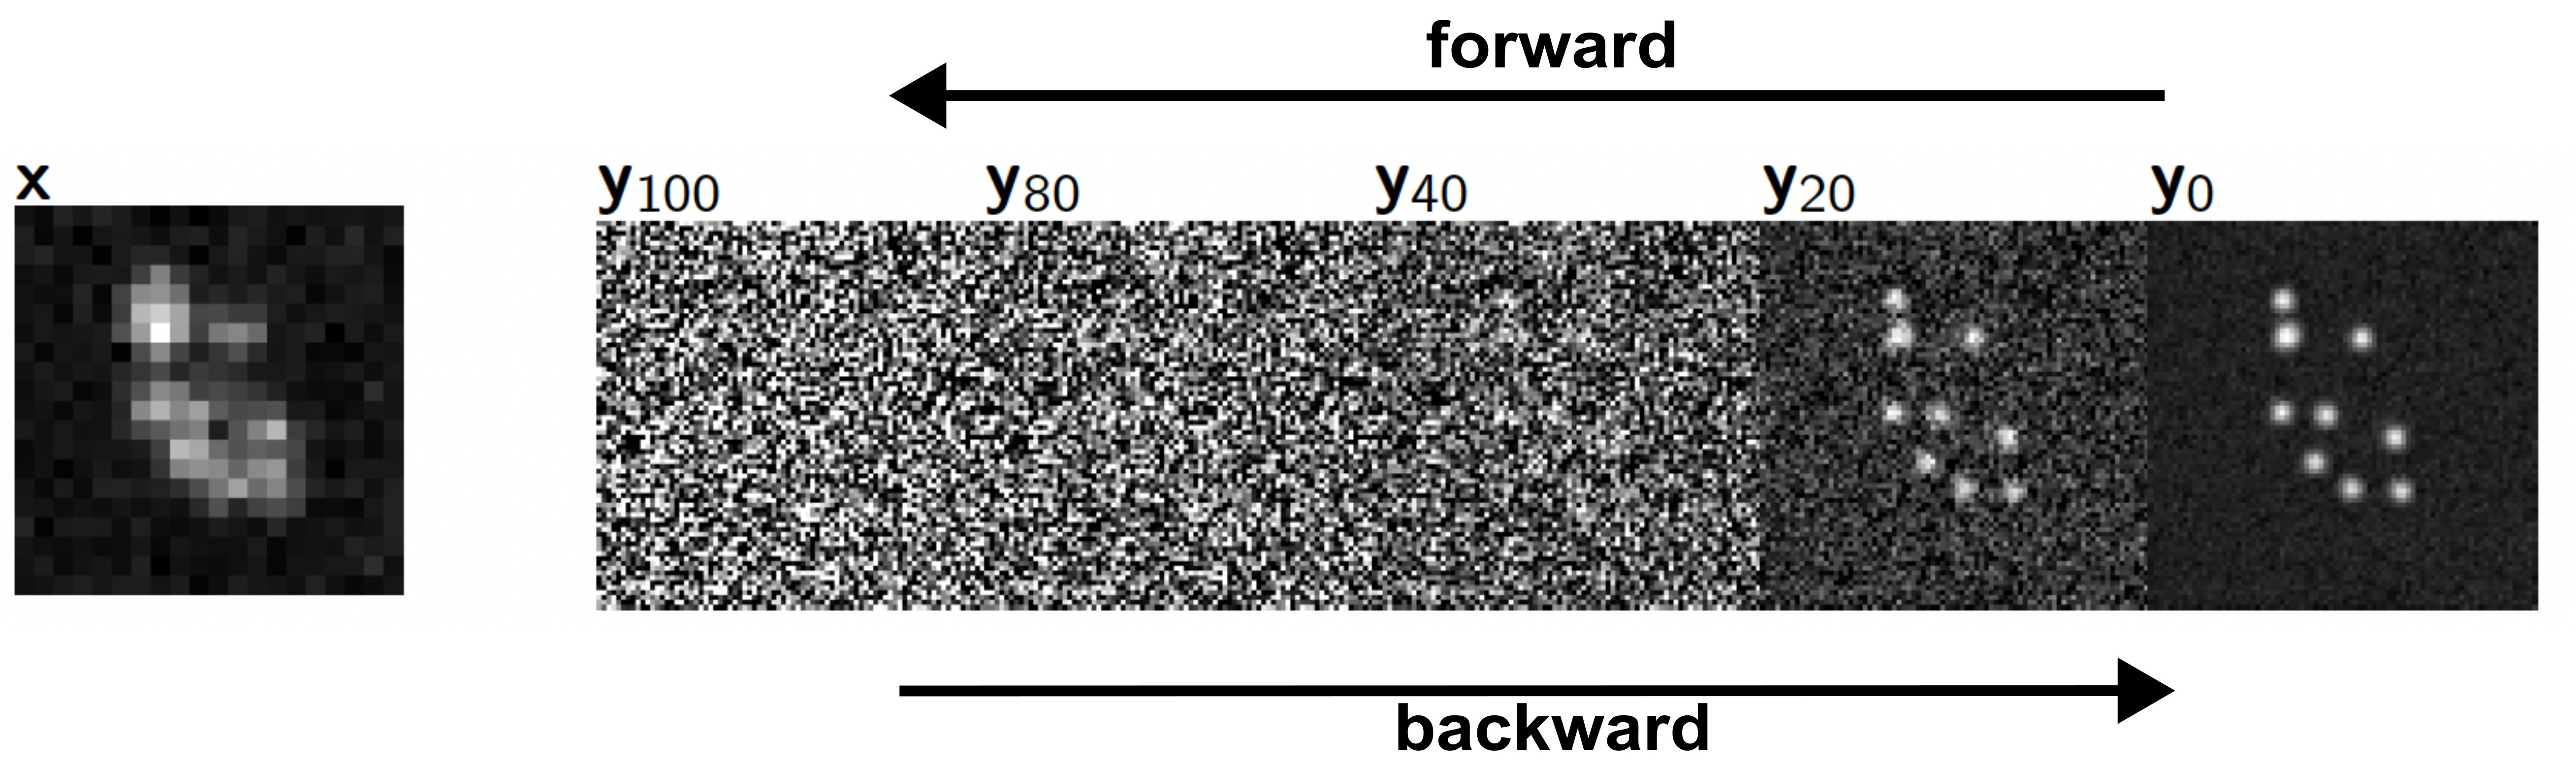
\includegraphics[width=12cm]{../../ddpm/ddpm/media/ForwardBackward.png}
\end{textblock*}

\begin{textblock*}{2cm}(6.5cm, 7.75cm)
\begin{equation*}
p_{\psi}(\bold{y}_{t-1}|\bold{y}_{t},\bold{x}) = \mathcal{N}\left(\mu_{\psi},\beta_{t}I\right)
\end{equation*}

\end{textblock*}

\end{frame}

\begin{frame}{Approach I: Resolution enhancement with a diffusion model}
\begin{textblock*}{9cm}(3.0cm, 2.0cm)
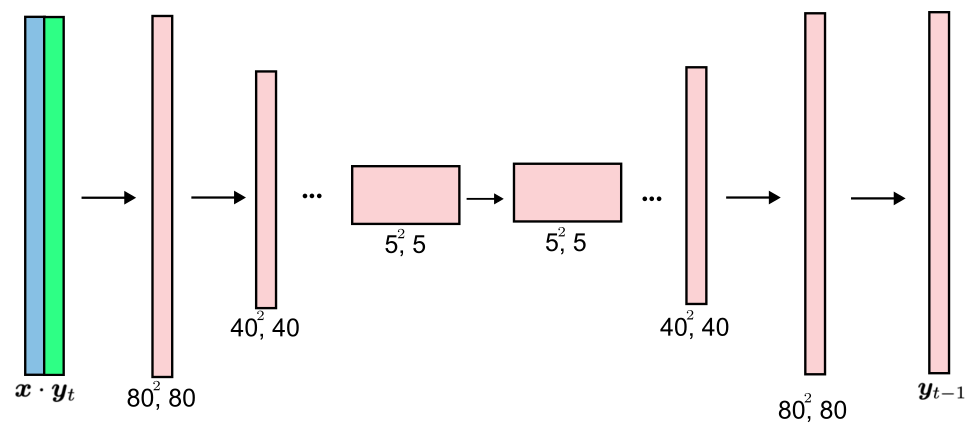
\includegraphics[width=9cm]{../../ddpm/ddpm/media/DiffusionArch.png}
\end{textblock*}
\begin{textblock*}{2cm}(0.5cm, 3.0cm)
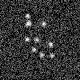
\includegraphics[width=2cm]{../../dissertation/dissertation/media/diffusion_example/0_1_sr_79.png}
\end{textblock*}
\begin{textblock*}{2cm}(12.5cm, 3.0cm)
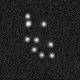
\includegraphics[width=2cm]{../../dissertation/dissertation/media/diffusion_example/0_1_sr_99.png}
\end{textblock*}

\begin{textblock*}{13cm}(1.0cm, 6.5cm)
\begin{itemize}
\item A convolutional neural network $\psi$ estimates the drift $\mu_{\psi}$
\item Denoising step: $y_{t-1}\sim p_{\psi}(\bold{y}_{t-1}|\bold{y}_{t},\bold{x}) = \mathcal{N}\left(\mu_{\psi},\beta_{t}I\right)$
\end{itemize}
\end{textblock*}
\end{frame}

\begin{comment}
\begin{frame}{Bayesian image restoration with diffusion models}

\begin{textblock*}{2cm}(1.0cm, 1.0cm)
$\bold{x}$
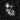
\includegraphics[width=2cm]{../../dissertation/dissertation/media/diffusion_example/Diffusion_lr-0.png}
\end{textblock*}
\begin{textblock*}{2cm}(4.0cm, 1.0cm)
$\bold{y}_{100}$

\includegraphics[width=2cm]{../../dissertation/dissertation/media/diffusion_example/0_1_sr_1.png}
\end{textblock*}
\begin{textblock*}{2cm}(6.0cm, 1.0cm)
$\bold{y}_{80}$

\includegraphics[width=2cm]{../../dissertation/dissertation/media/diffusion_example/0_1_sr_19.png}
\end{textblock*}
\begin{textblock*}{2cm}(8.0cm, 1.0cm)
$\bold{y}_{40}$

\includegraphics[width=2cm]{../../dissertation/dissertation/media/diffusion_example/0_1_sr_39.png}
\end{textblock*}
\begin{textblock*}{2cm}(10.0cm,1.0cm)
$\bold{y}_{20}$
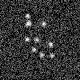
\includegraphics[width=2cm]{../../dissertation/dissertation/media/diffusion_example/0_1_sr_79.png}
\end{textblock*}
\begin{textblock*}{2cm}(12.0cm, 1.0cm)
$\bold{y}_{0}$
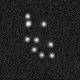
\includegraphics[width=2cm]{../../dissertation/dissertation/media/diffusion_example/0_1_sr_99.png}
\end{textblock*}

\begin{textblock*}{10cm}(2.0cm, 4.0cm)

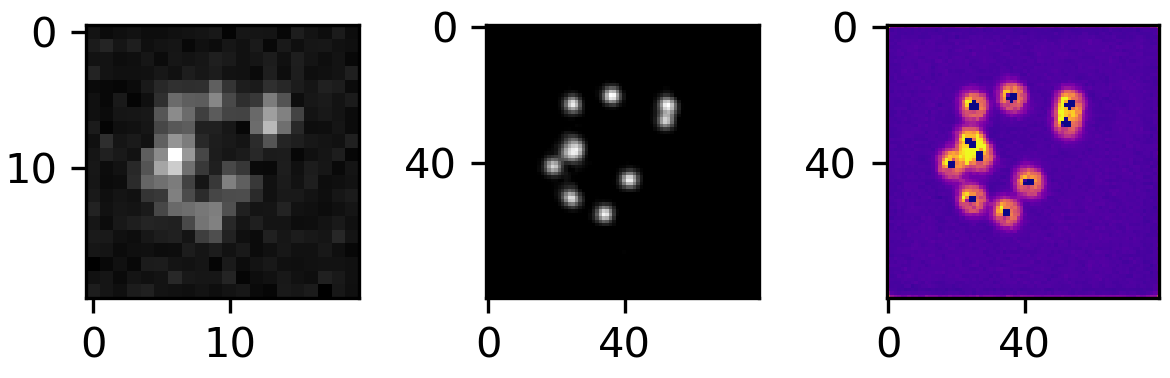
\includegraphics[width=10cm]{../../dissertation/dissertation/media/Bayes.png}
\end{textblock*}

\begin{textblock*}{12cm}(1.0cm, 7.5cm)
Estimation of pixel-wise uncertainty in the high resolution $\bold{y}$
\end{textblock*}


\end{frame}
\end{comment}

\begin{frame}{Super resolution of BRD4 protein in a HeLa cell}
\begin{textblock*}{12cm}(2.0cm,1.5cm)
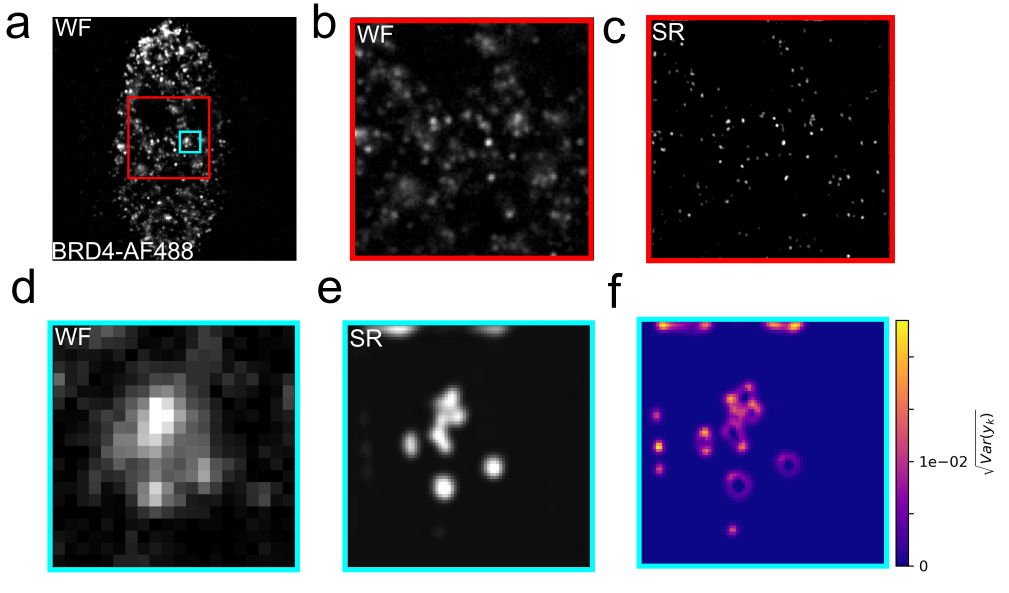
\includegraphics[width=12cm]{../../ddpm/ddpm/media/BRD4/Deep2.png}
\end{textblock*}


\end{frame}

\subsection{Approach II: Integrated single photon counting and widefield single molecule imaging}

\begin{frame}{Approach II: Integrated single photon counting and widefield single molecule imaging}
\begin{itemize}
\item Single photon avalanche diode (SPAD) arrays give us new modeling approaches
\end{itemize}
%\begin{textblock*}{13cm}(1.0cm,1.0cm)
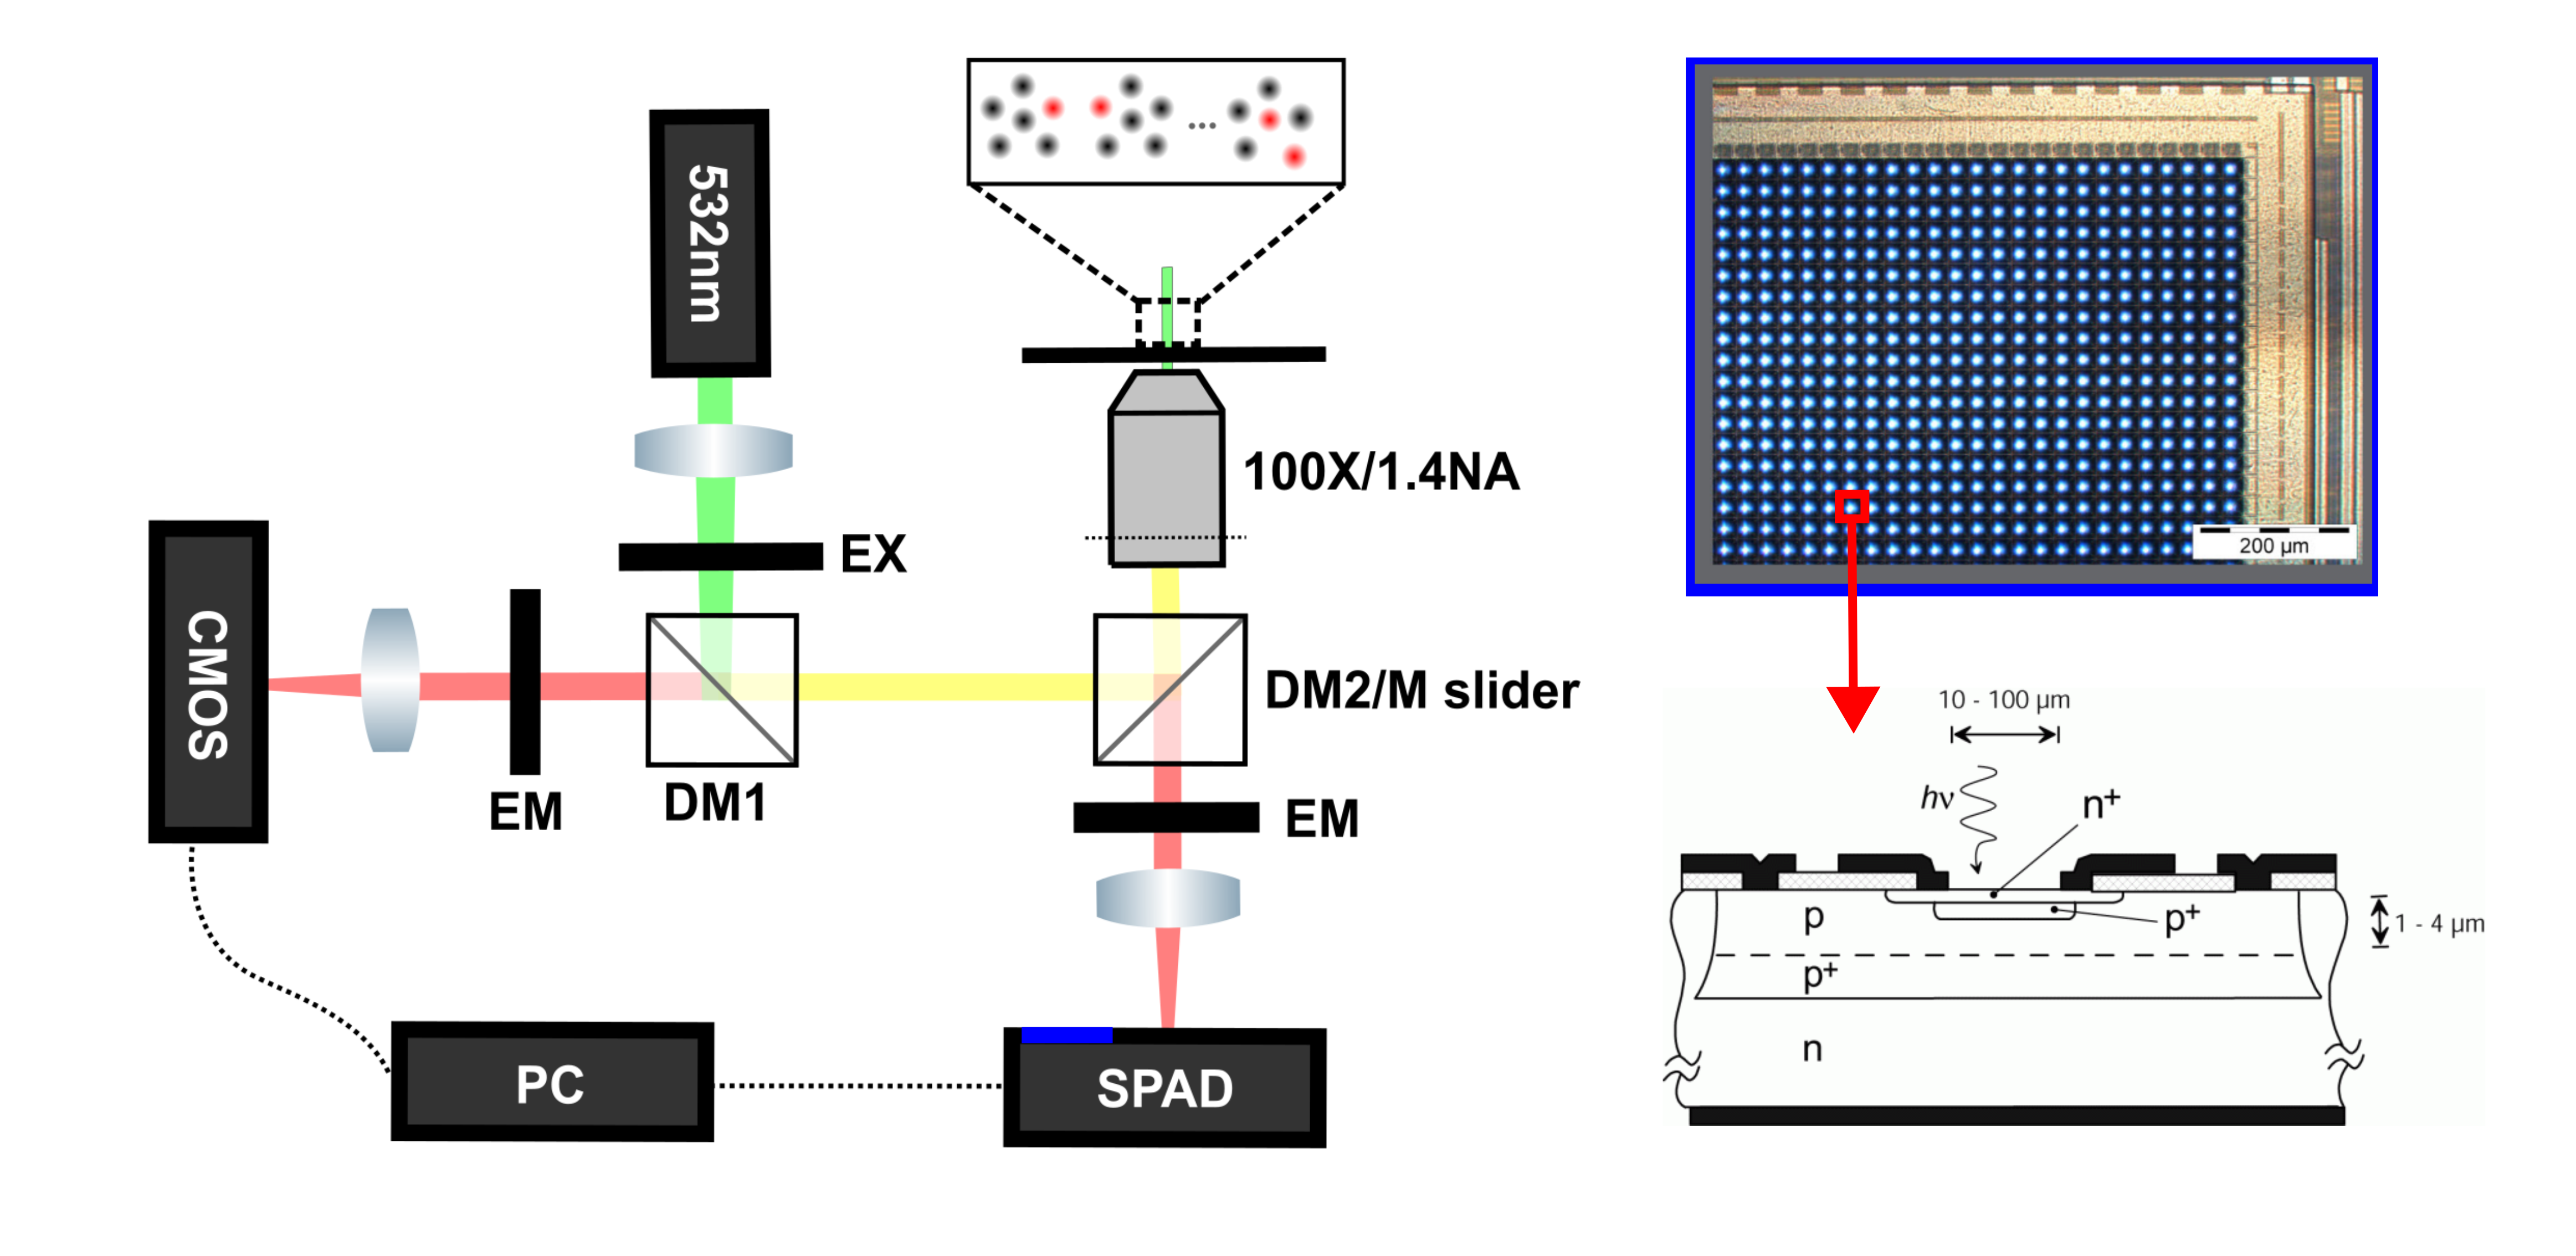
\includegraphics[width=13cm]{../../spad/spad/media/SPADD.png}
%\end{textblock*}
\end{frame}

\begin{comment}
\begin{frame}{The Hanbury Brown and Twiss Effect}
\begin{textblock*}{13cm}(1.0cm,1.0cm)
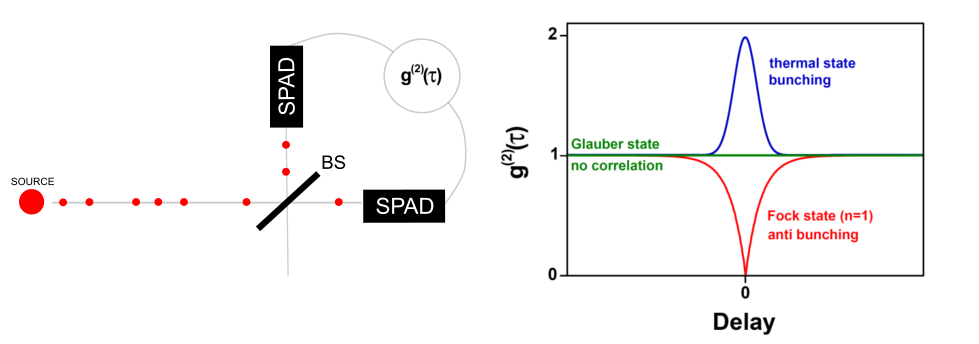
\includegraphics[width=13cm]{../../spad/spad/media/HBT.png}
\end{textblock*}

\begin{textblock*}{13cm}(1.0cm,6.0cm)
\begin{equation*}
g^{(2)}(\tau) = \frac{\langle n(t) n(t+\tau) \rangle}{\langle n(t) \rangle^2}
\end{equation*}

\begin{itemize}
\item Single photon sources (such as a fluorescent dye) exhibit antibunching
\item Magnitude of $g^{(2)}(0)$ "dip" depends on the number of fluorescent emitters
\end{itemize}
\end{textblock*}

\end{frame}
\end{comment}

%\begin{frame}{Widefield photon counting with a SPAD array}
%\begin{textblock*}{13cm}(1.0cm,1.0cm)
%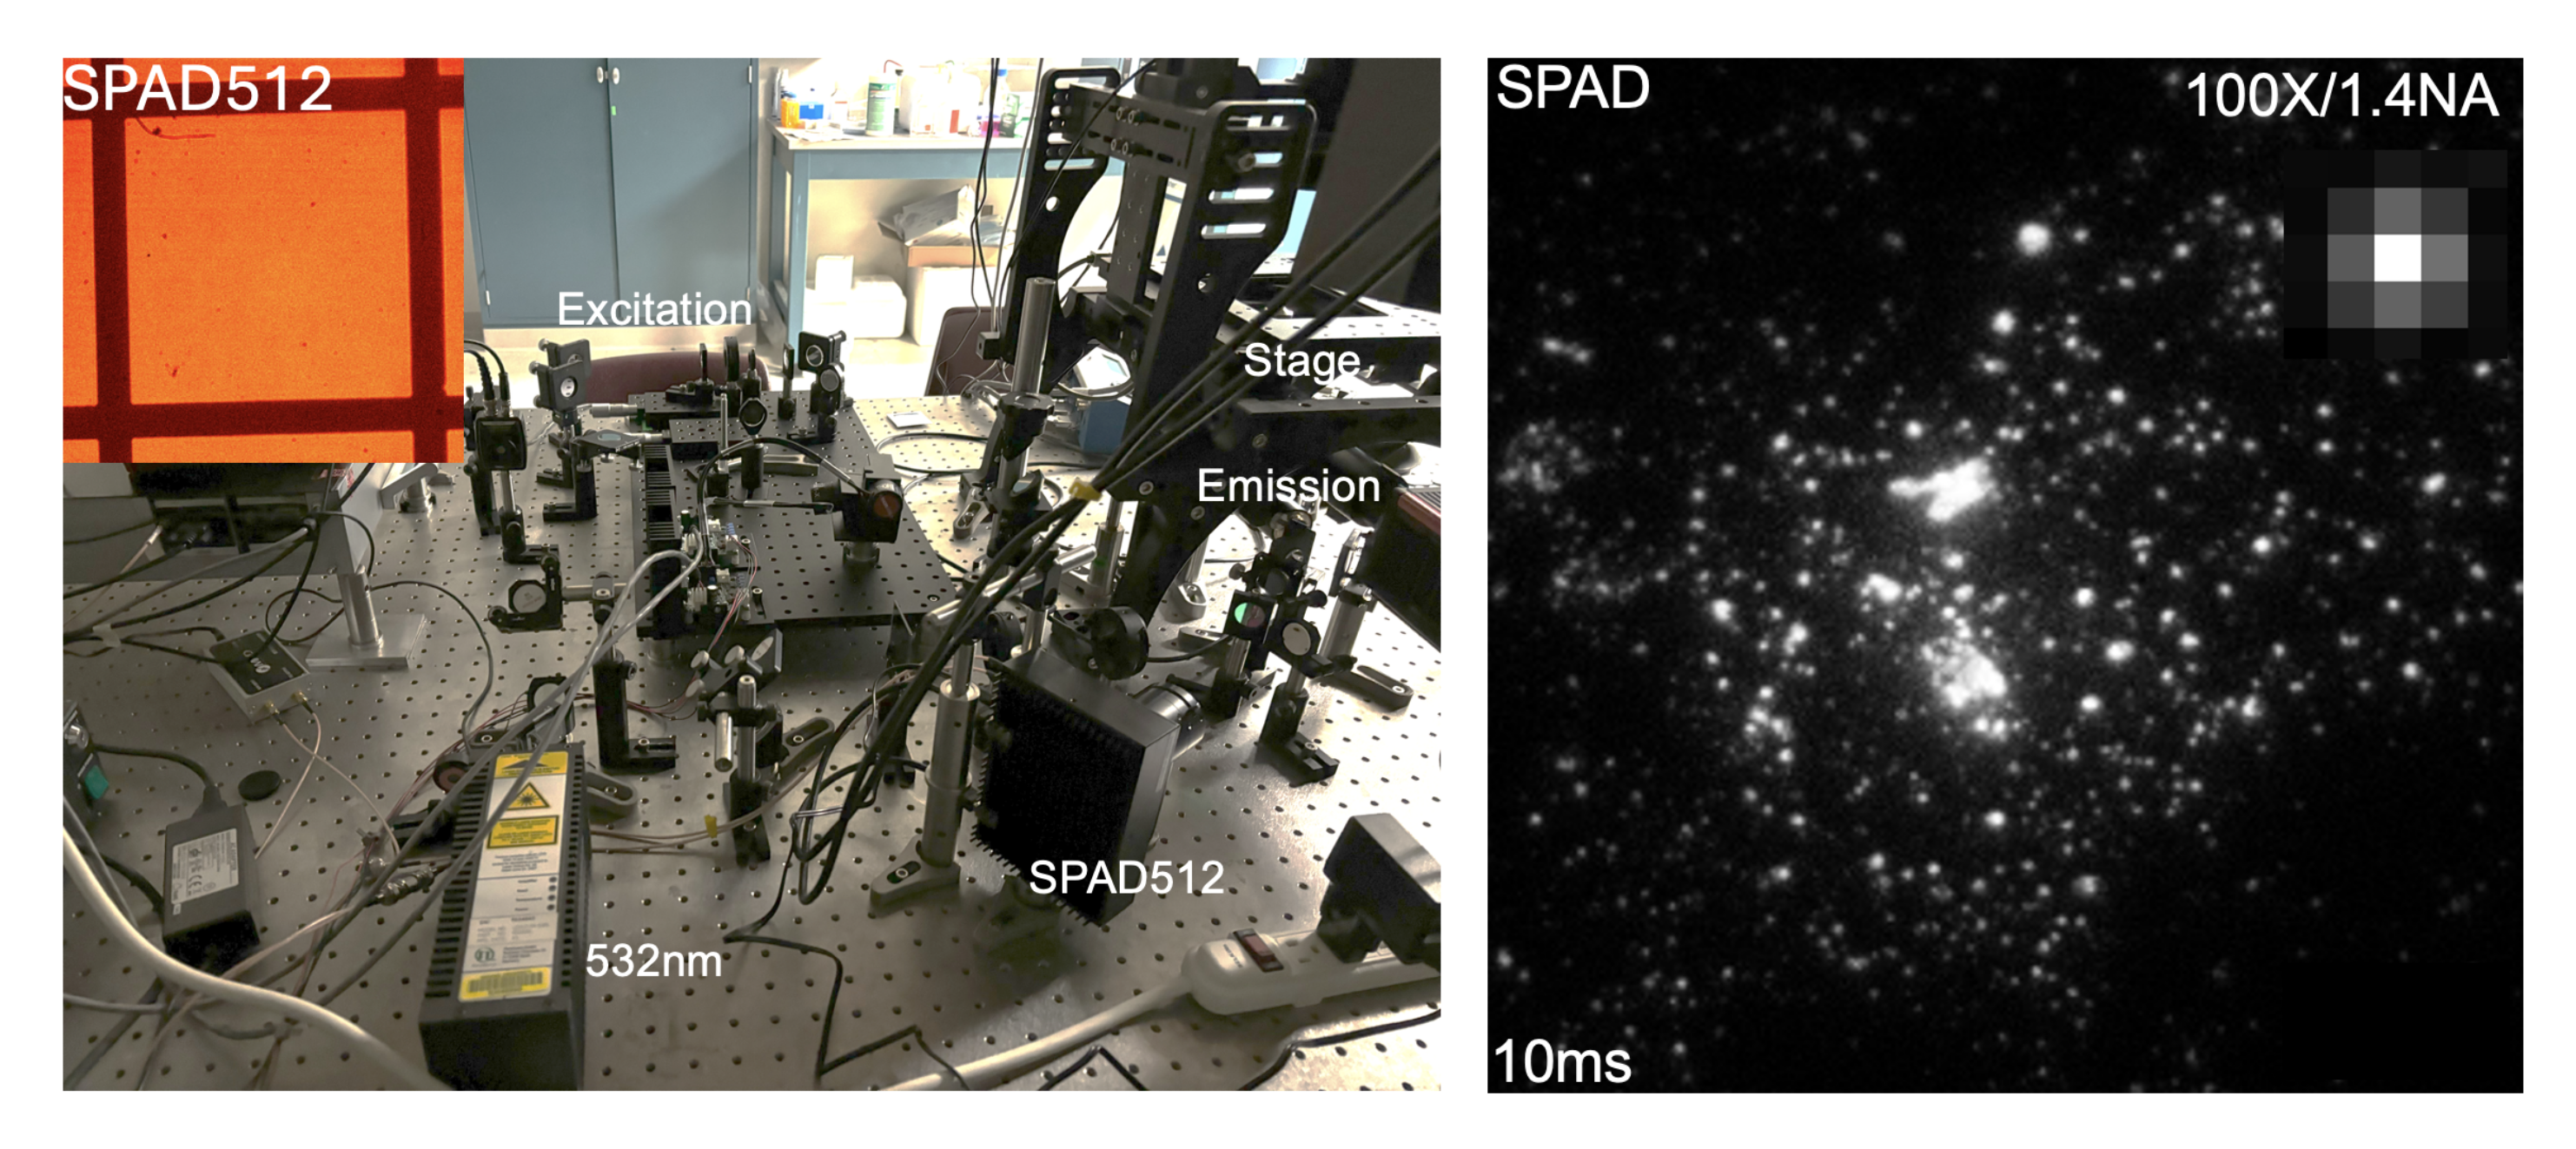
\includegraphics[width=13cm]{../../spad/spad/media/Widefield.png}
%\end{textblock*}
%\begin{textblock*}{13cm}(1.0cm,7.0cm)

%\begin{itemize}
%\item Spatial resolution of photon counts
%\item Fast exposures as low as 20 nanoseconds
%\end{itemize}
%\end{textblock*}
%\end{frame}

\begin{frame}{Imaging Qdot655 photon by photon}
\begin{textblock*}{12cm}(1.0cm,1.5cm)
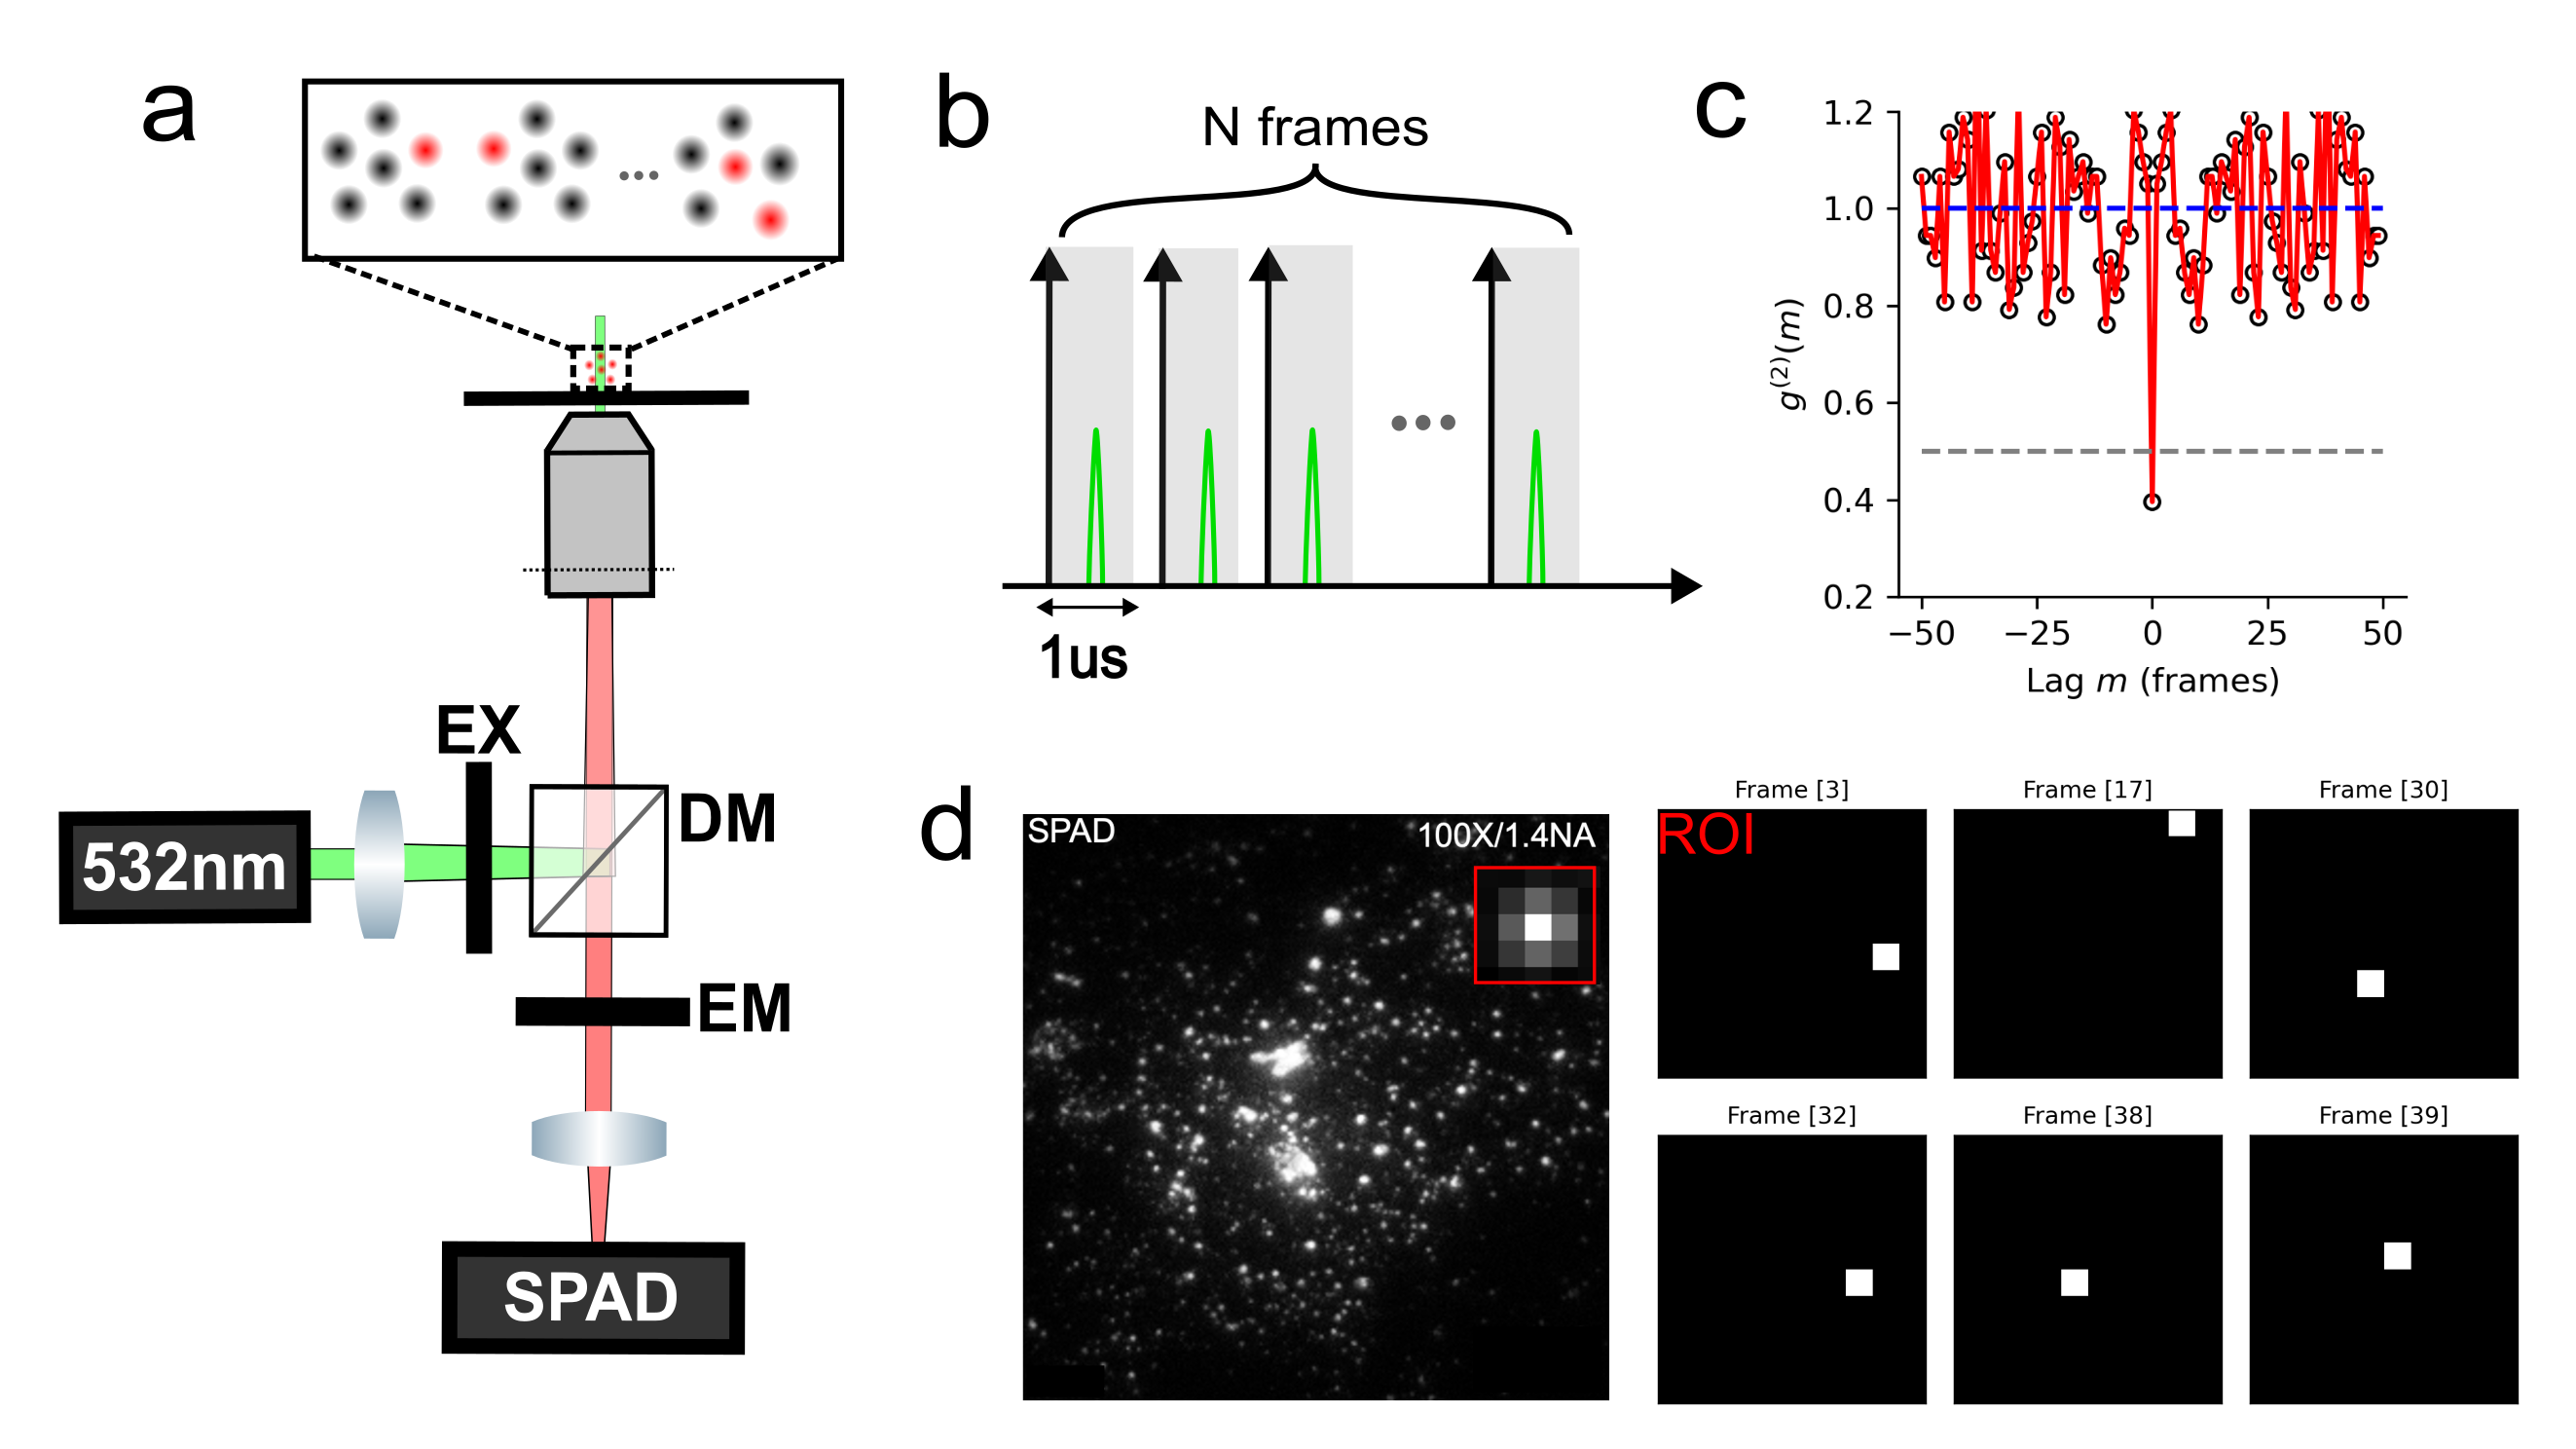
\includegraphics[width=12cm]{../../spad/spad/media/Figure-0.png}
\end{textblock*}
\begin{textblock*}{13cm}(1.0cm,8.5cm)
\begin{itemize}
\item $g^{(2)}(m) = G^{(2)}(0)/\langle G^{(2)}(m)\rangle$
%\item 532nm picosecond pulsed laser pulsed at 500kHz to excite fluorescent quantum dots
\end{itemize}
\end{textblock*}

\end{frame}

\begin{frame}{Poisson-Binomial photon count data (simulation)}
\begin{textblock*}{10cm}(2.0cm,1.0cm)
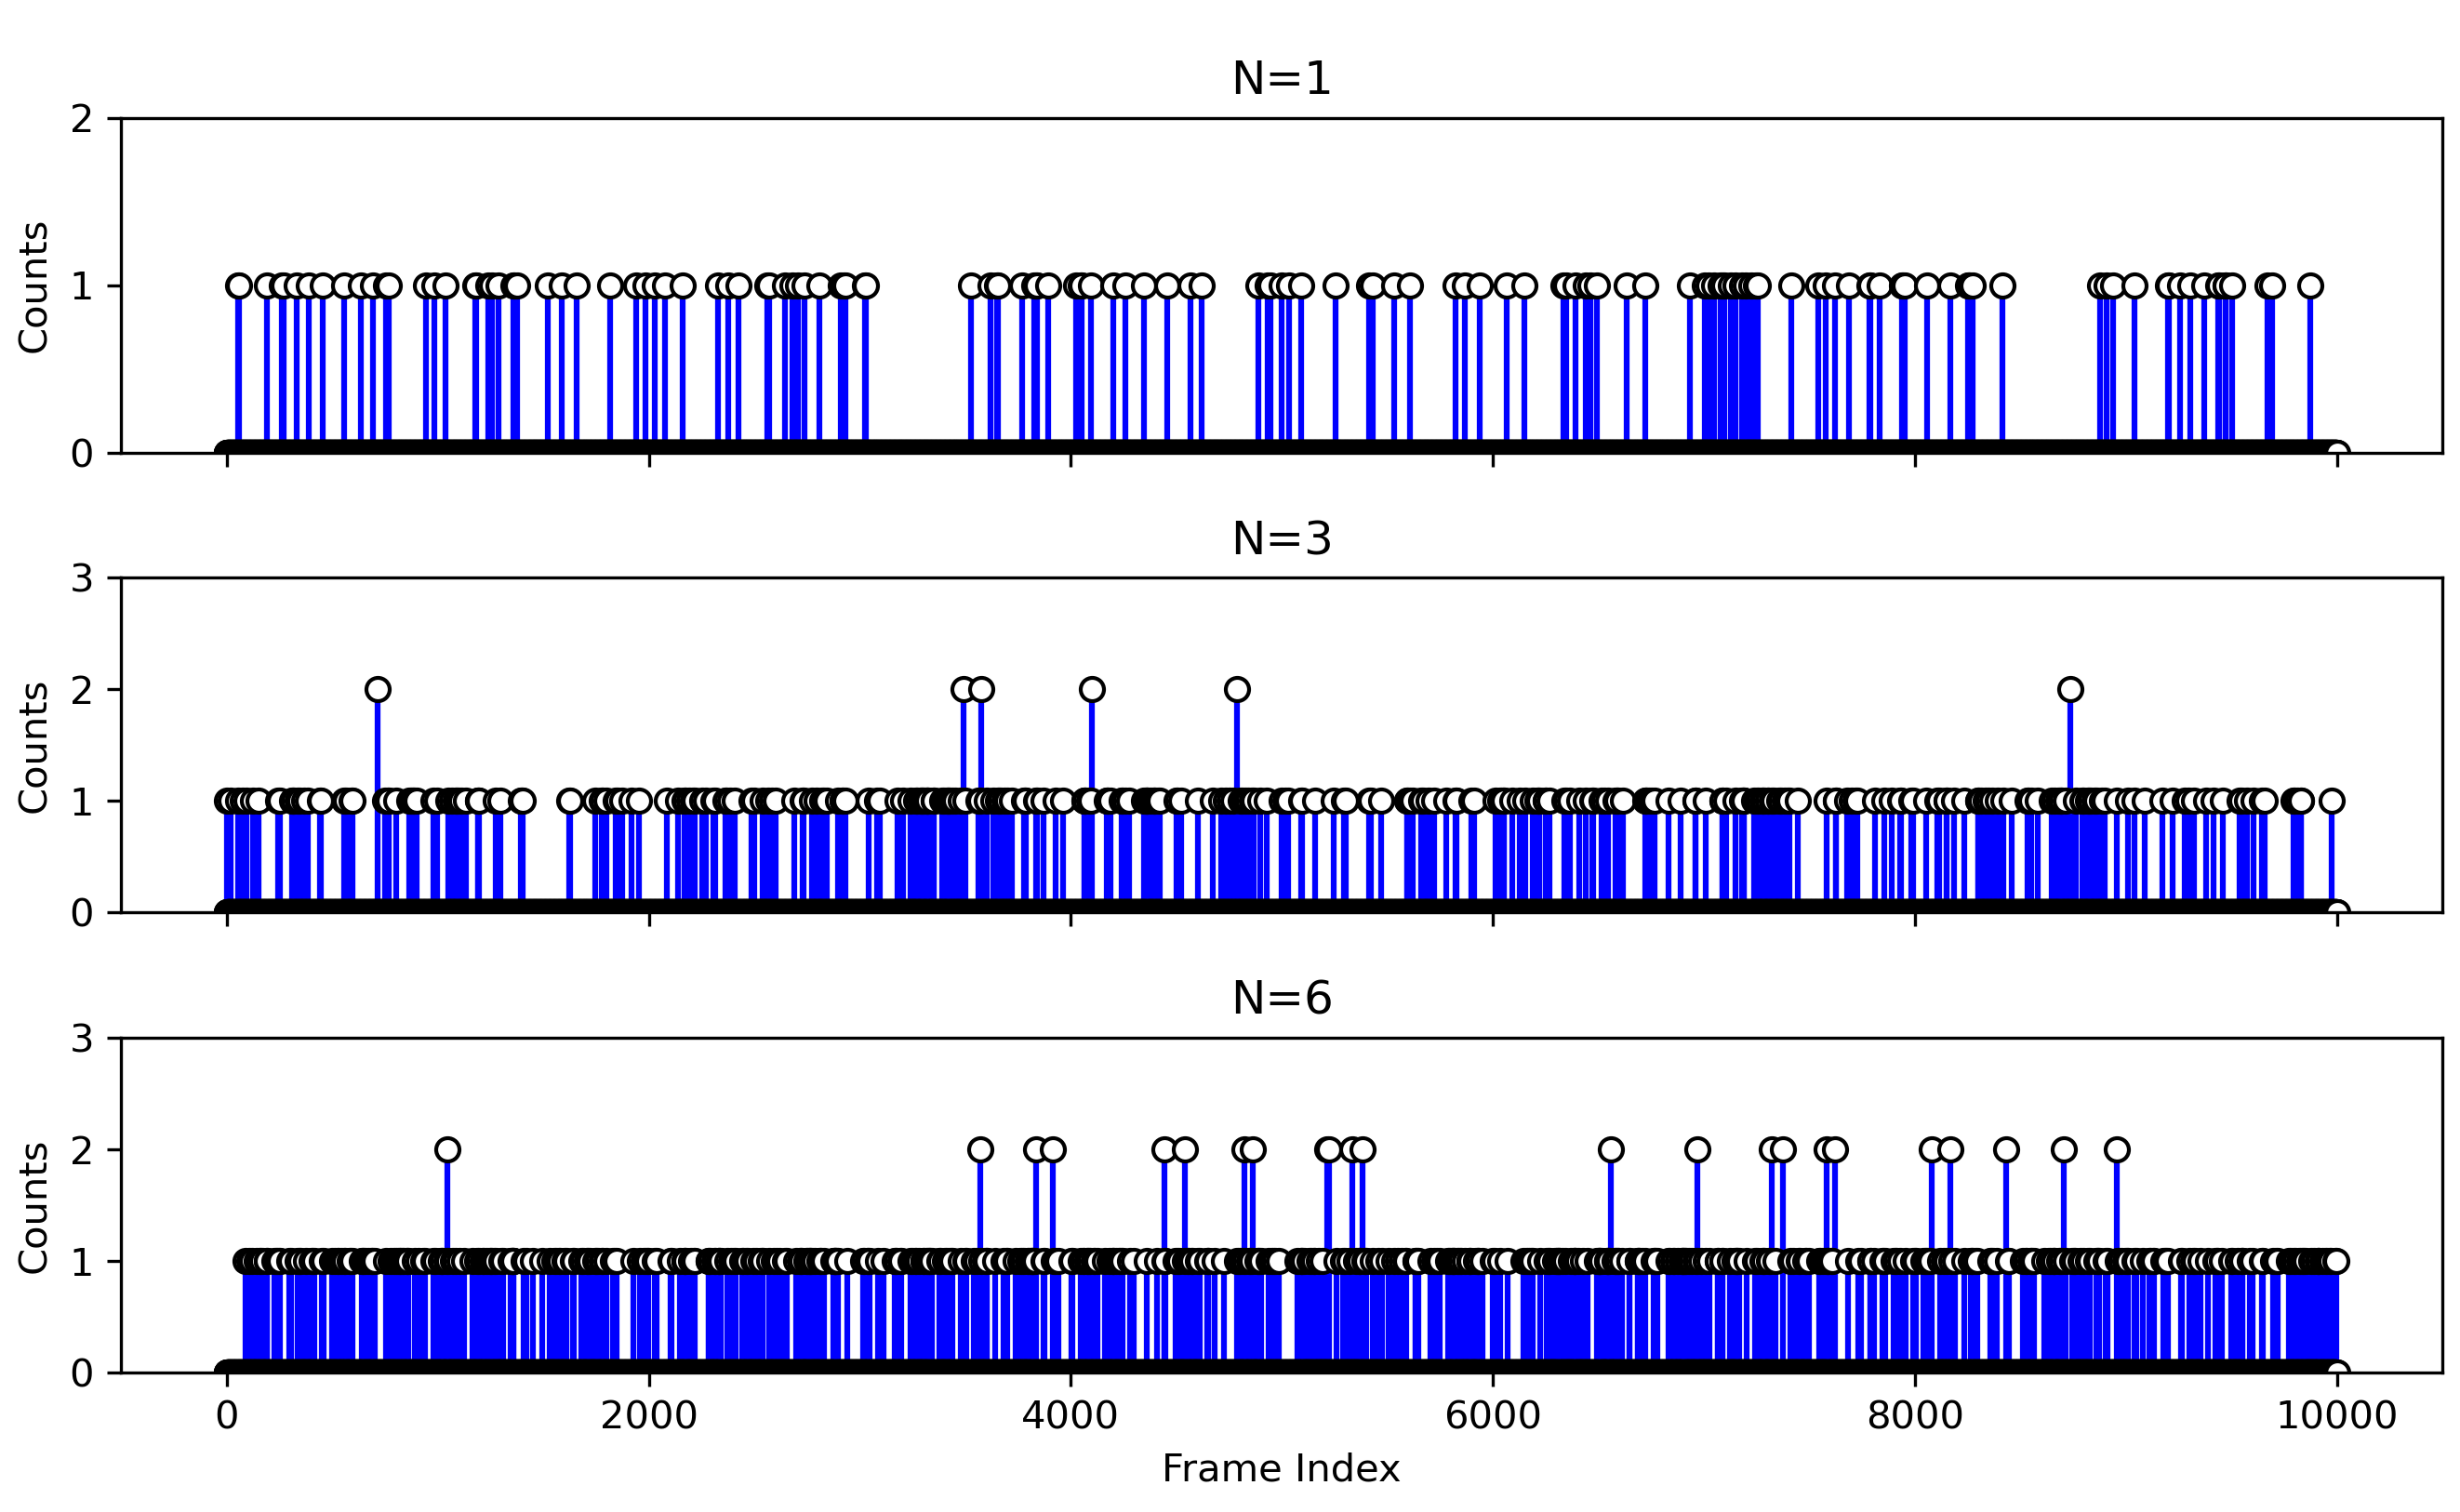
\includegraphics[width=10cm]{../../spad/spad/media/Counts.png}
\end{textblock*}
\begin{textblock*}{13cm}(1.0cm,7.5cm)
\begin{itemize}
\item SPAD arrays permit modeling of time-series of photon counts $n_{t}$
\item Likelihood on counts: $\mathcal{L}(n_t\lvert N,\zeta,\lambda) = \mathrm{Poisson}(\lambda)* \mathrm{Binomial}(N,\zeta)$
\end{itemize}
\end{textblock*}

\end{frame}

\begin{frame}{Discrimination of single and multiple quantum dots}
%\begin{textblock*}{13cm}(2.0cm,1.0cm)
\begin{center}
\includegraphics[width=13cm]{../../spad/spad/media/CountQD.png}
\end{center}
%\end{textblock*}
\begin{textblock*}{14cm}(1.0cm,9.0cm)
%Posterior on $N$: $p(N\lvert n_t) \propto \int_{0}^{1} \mathcal{L}(n_t\lvert N,\zeta)p(\zeta)d\zeta$
Blinking in quantum dots occurs due to non-radiative relaxation pathways
\end{textblock*}

\end{frame}

\begin{comment}
\begin{frame}{Constrained multi-emitter localization with photon counting}

\begin{textblock*}{7cm}(1.0cm,1.5cm)
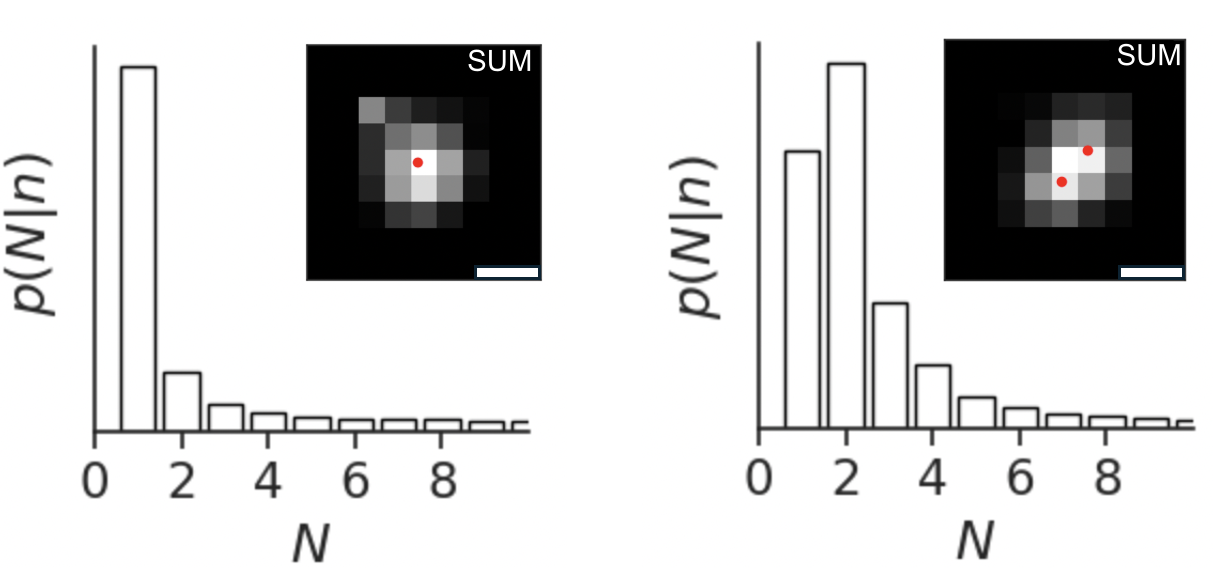
\includegraphics[width=7cm]{../../spad/spad/media/Figure-4.png}
\end{textblock*}

\begin{textblock*}{7cm}(1.0cm,5.0cm)
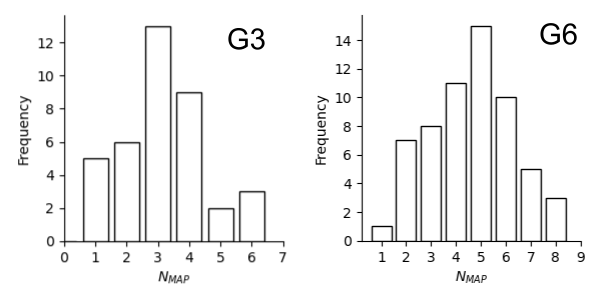
\includegraphics[width=7cm]{../../spad/spad/media/Figure-5.png}
\end{textblock*}


\begin{textblock*}{6cm}(8.5cm,2.5cm)
\begin{itemize}
\item $p(N|n)\rightarrow$ parameterization of multi-emitter fitting
\end{itemize}
\end{textblock*}

\begin{textblock*}{6cm}(8.5cm,5.5cm)
\begin{itemize}
\item Sampling based multi-emitter fitting
\item Approaches lower bound on localization error at high counts
\end{itemize}
\end{textblock*}

\end{frame}

\begin{frame}{Constrained multi-emitter localization with photon counting}

\begin{textblock*}{7cm}(1.0cm,1.5cm)
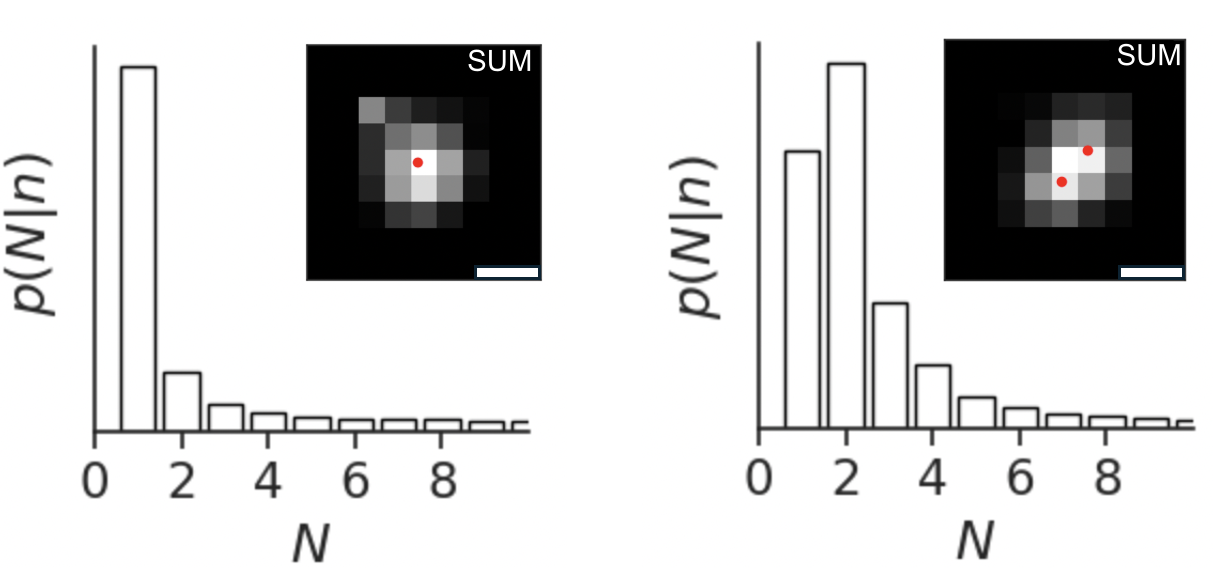
\includegraphics[width=7cm]{../../spad/spad/media/Figure-4.png}
\end{textblock*}

\begin{textblock*}{7cm}(1.0cm,5.0cm)
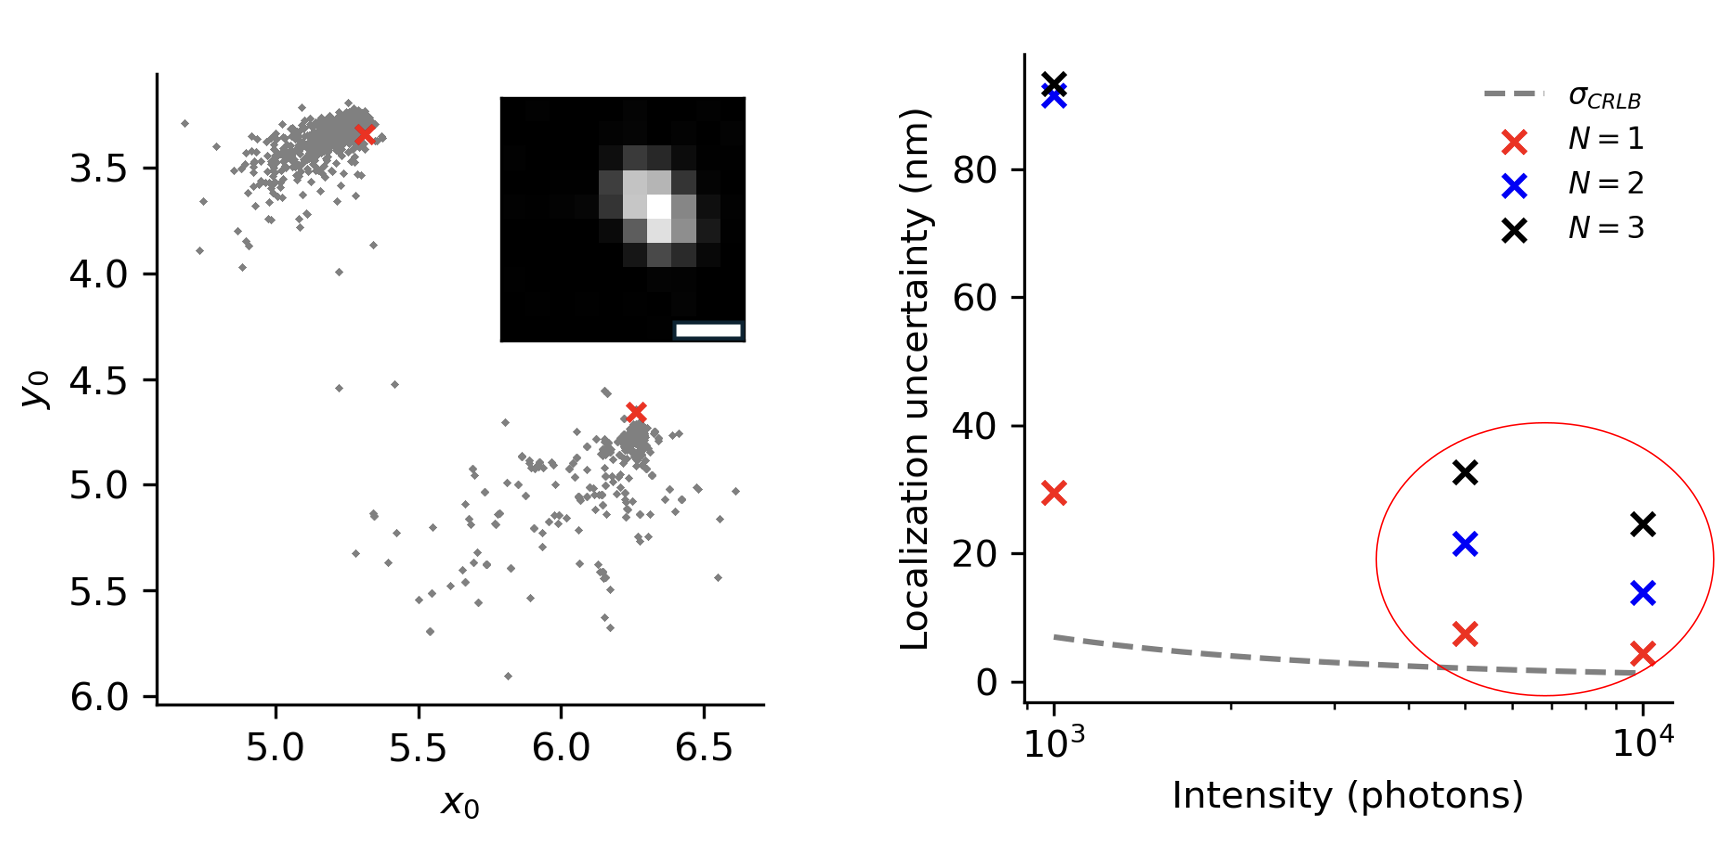
\includegraphics[width=7cm]{../../spad/spad/media/Figure-5-2.png}
\end{textblock*}


\begin{textblock*}{6cm}(8.5cm,2.5cm)
\begin{itemize}
\item $p(N|n)\rightarrow$ parameterization of multi-emitter fitting
\end{itemize}
\end{textblock*}

\begin{textblock*}{6cm}(8.5cm,5.5cm)
\begin{itemize}
\item Sampling based multi-emitter fitting
\item Approaches lower bound on localization error at high counts
\end{itemize}
\end{textblock*}

\end{frame}

\end{comment}

\begin{frame}{Constrained multi-emitter localization (simulation)}

\begin{textblock*}{13cm}(1.0cm,1.5cm)
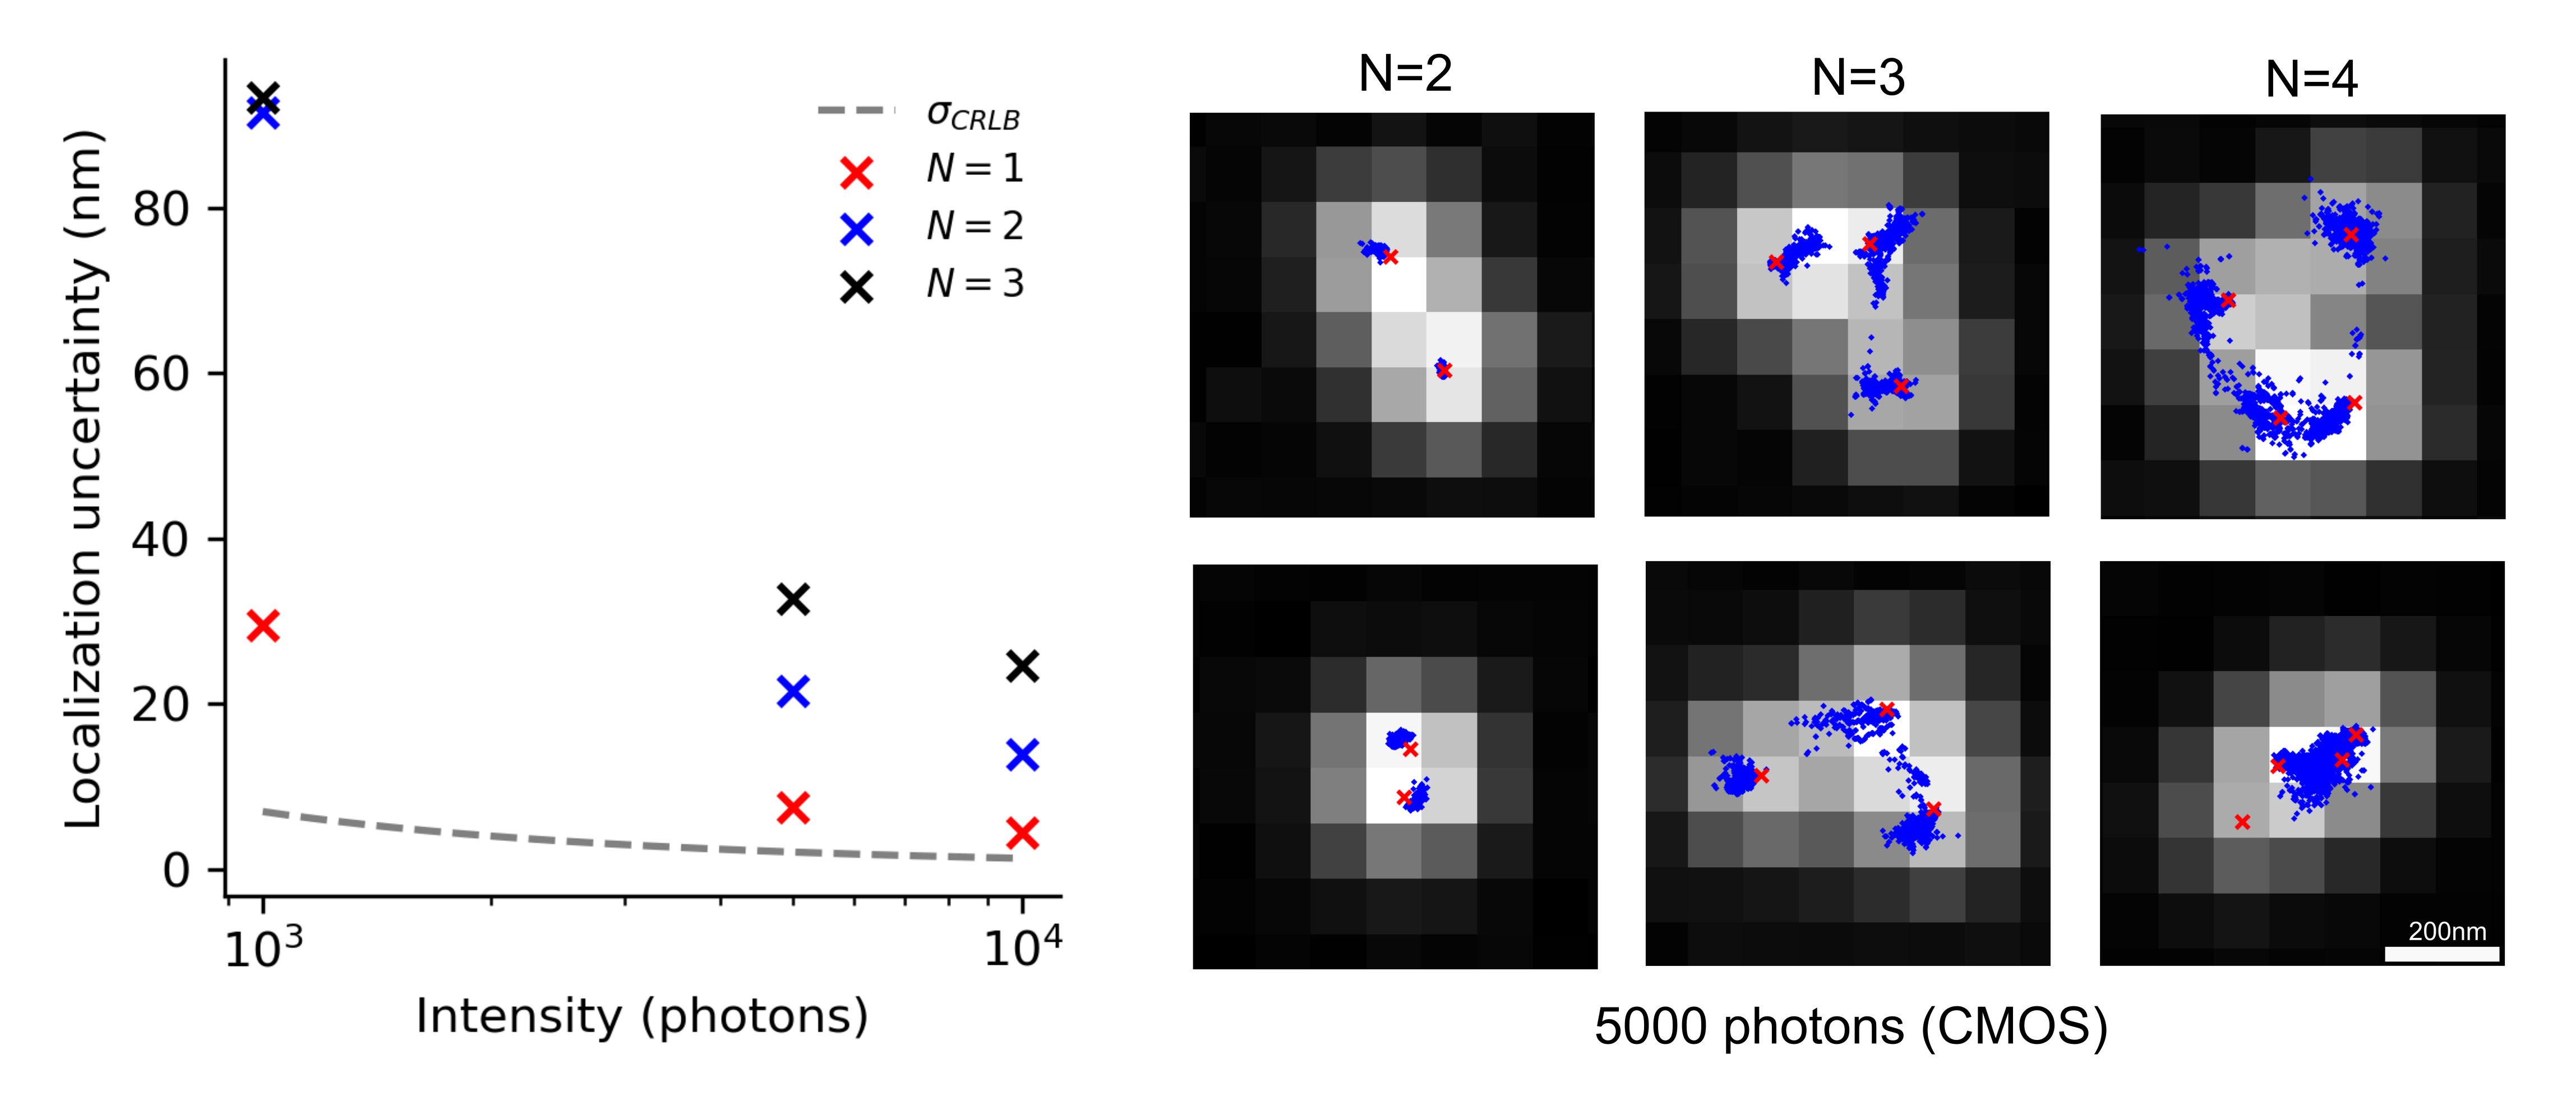
\includegraphics[width=13cm]{../../spad/spad/media/MultiEmitter.png}
\end{textblock*}

\begin{textblock*}{13cm}(1.0cm,8.0cm)
\begin{itemize}
\item Multiple emitters can be fit simultaneously using MCMC sampling
\item Constrained multi-emitter localization when $N$ is known
\end{itemize}
\end{textblock*}

\end{frame}


\begin{frame}{Upcoming work: counting ATTO532 dye bound to DNA origamis}
\begin{textblock*}{7cm}(1.0cm,1.3cm)
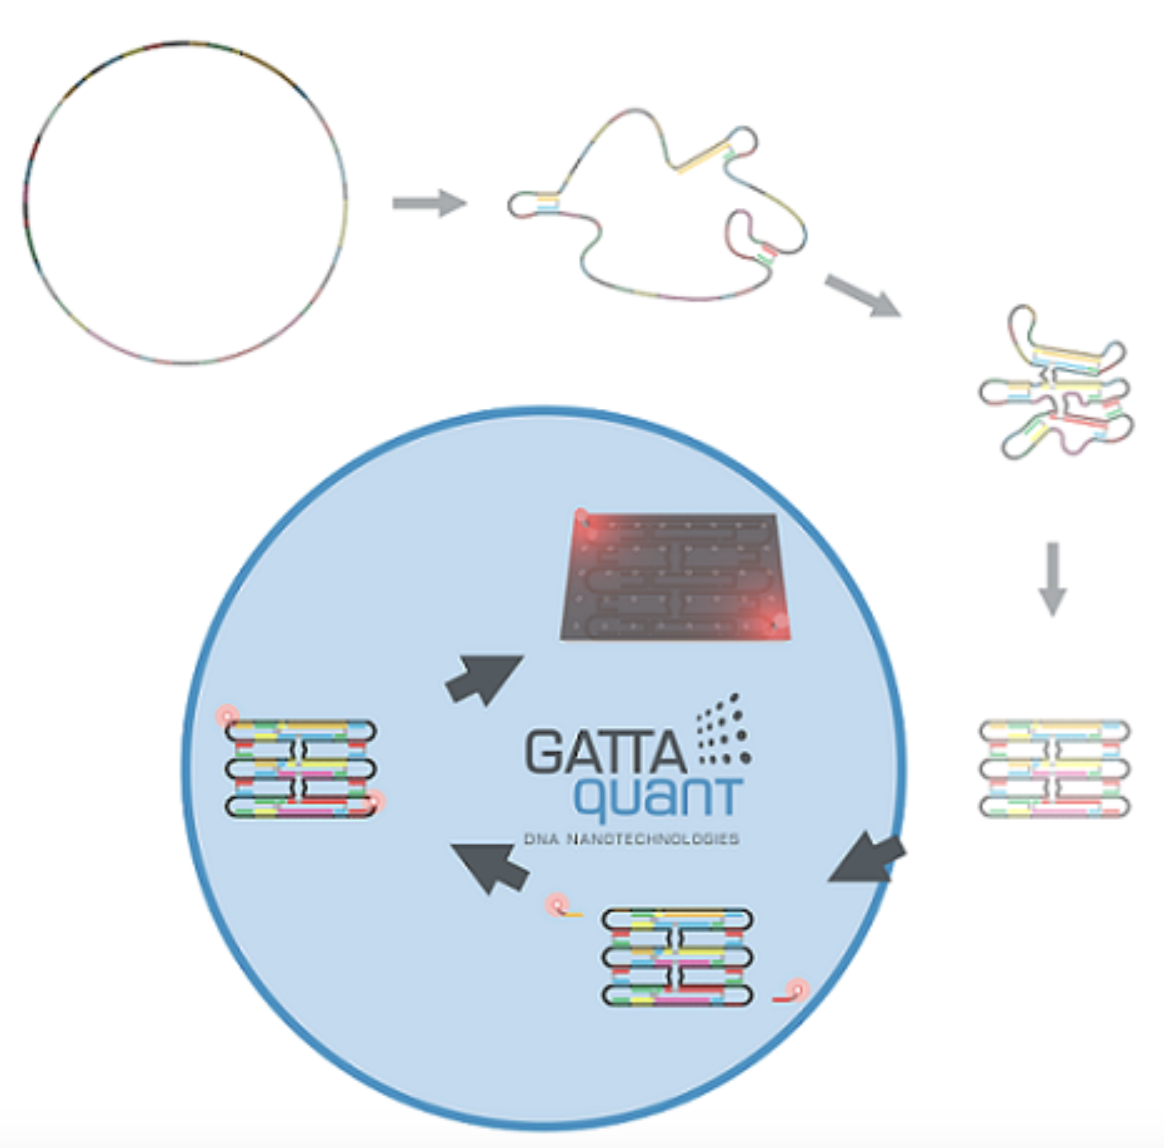
\includegraphics[width=7cm]{../../spad/spad/media/GATTA2.png}
\end{textblock*}
\begin{textblock*}{8cm}(1.0cm,8.5cm)
\textit{Courtesy of GATTAquant DNA Nanotech}
\end{textblock*}
\begin{textblock*}{7cm}(8.5cm,6.5cm)
\begin{itemize}
\item DNA origami 2um grid
\item Each binds $N$ ATTO532 dyes
\item Verification of counting method
\end{itemize}
\end{textblock*}
\begin{textblock*}{4.5cm}(9.0cm,1.0cm)
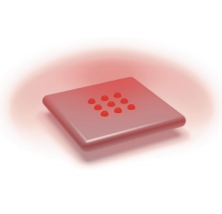
\includegraphics[width=4.5cm]{../../spad/spad/media/9R.png}
\end{textblock*}
\end{frame}


\begin{comment}
\begin{frame}{Heralding single photons with parametric downconversion}
\begin{textblock*}{4.5cm}(1.5cm,1.3cm)
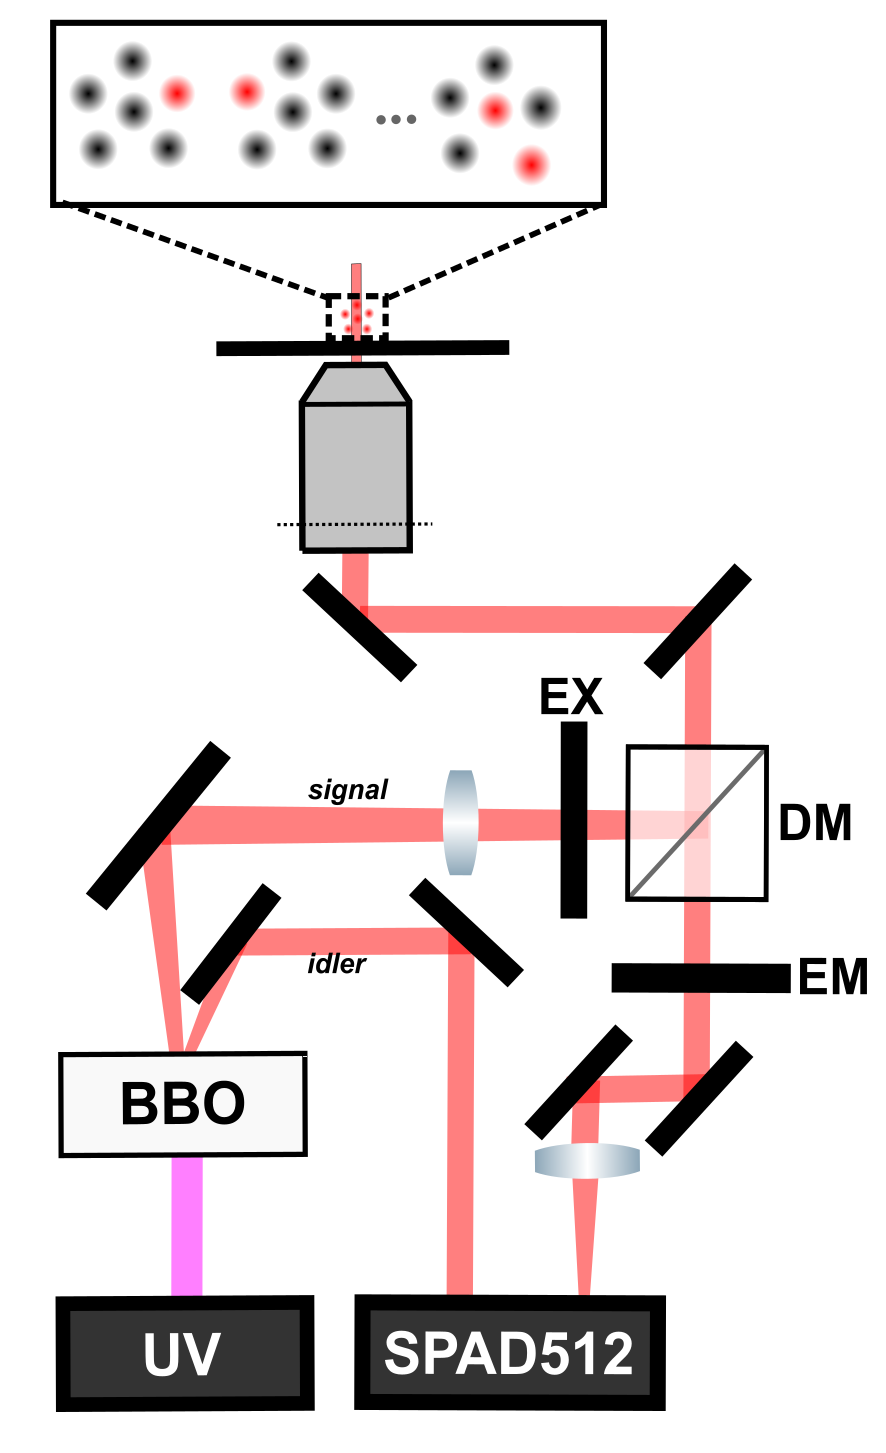
\includegraphics[width=4.5cm]{../../spad/spad/media/SPDC-Setup.png}
\end{textblock*}
\begin{textblock*}{6cm}(7.5cm,2.0cm)
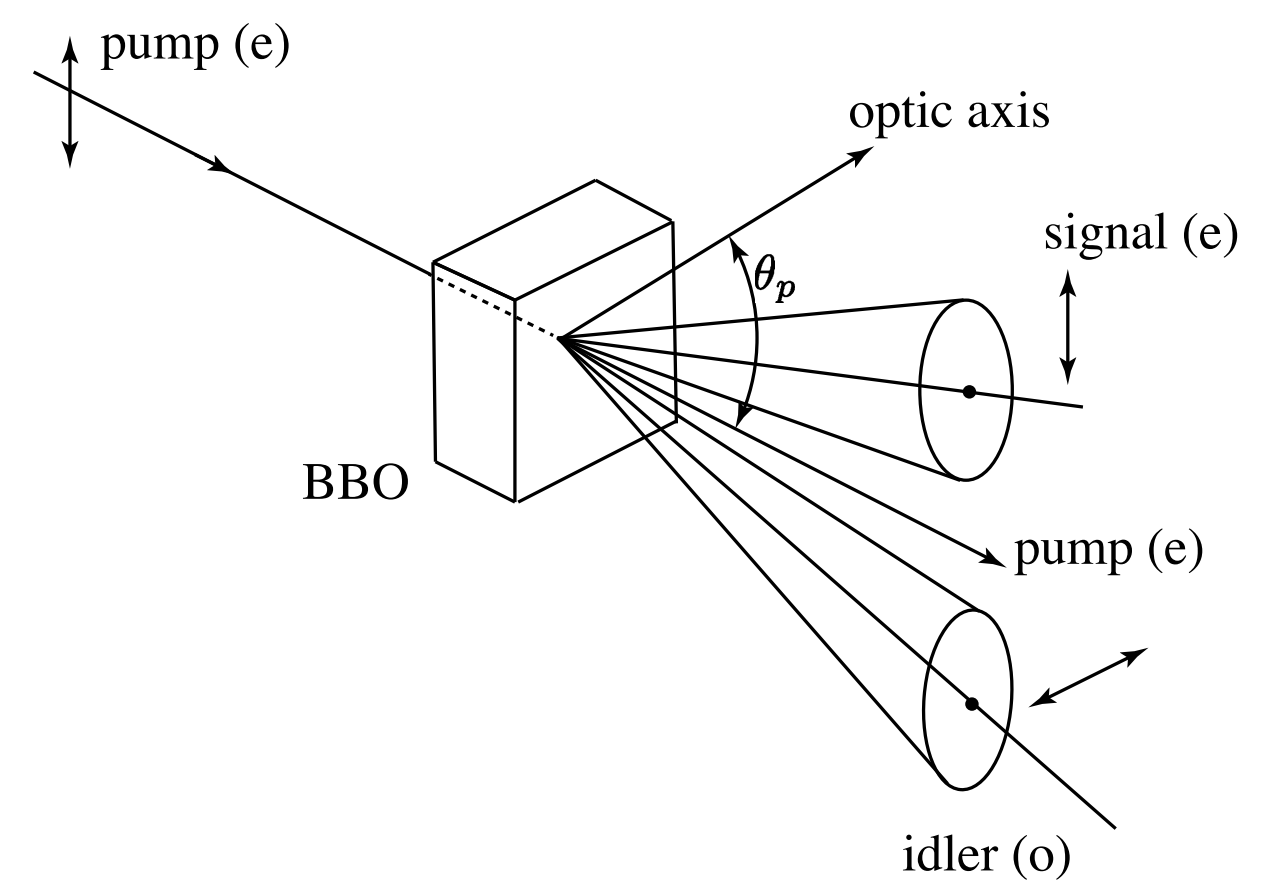
\includegraphics[width=6cm]{../../spad/spad/media/SPDC.png}
\end{textblock*}
\begin{textblock*}{2cm}(7cm,5.5cm)
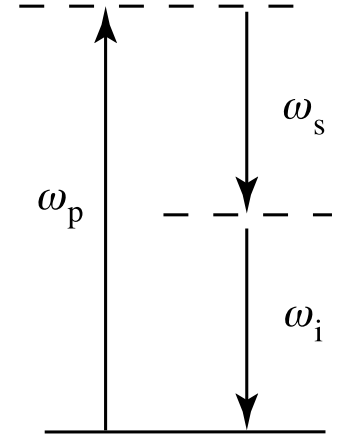
\includegraphics[width=2cm]{../../spad/spad/media/SPDC-2.png}
\end{textblock*}
\end{frame}

\begin{frame}{Heralding single photons with parametric downconversion}
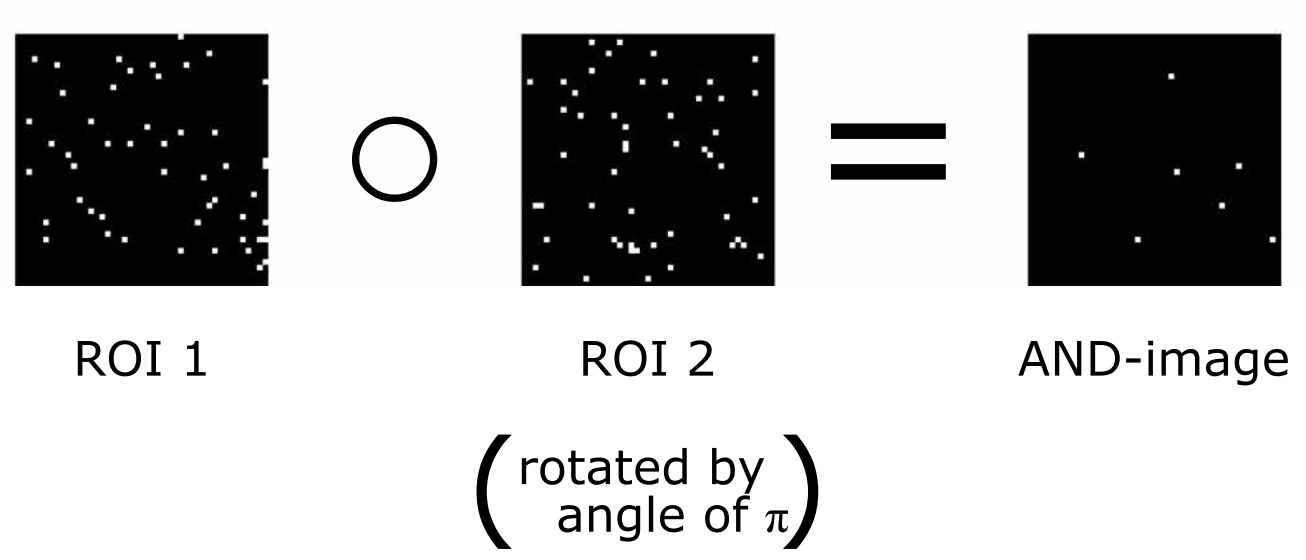
\includegraphics[width=10cm]{../../spad/spad/media/AND.png}

\begin{itemize}
\item Detection of dark counts or background counts
\item Noise free nanoscopy
\end{itemize}

\end{frame}
\end{comment}


%\begin{frame}{Inference of a high-resolution image from a low-resolution one}
%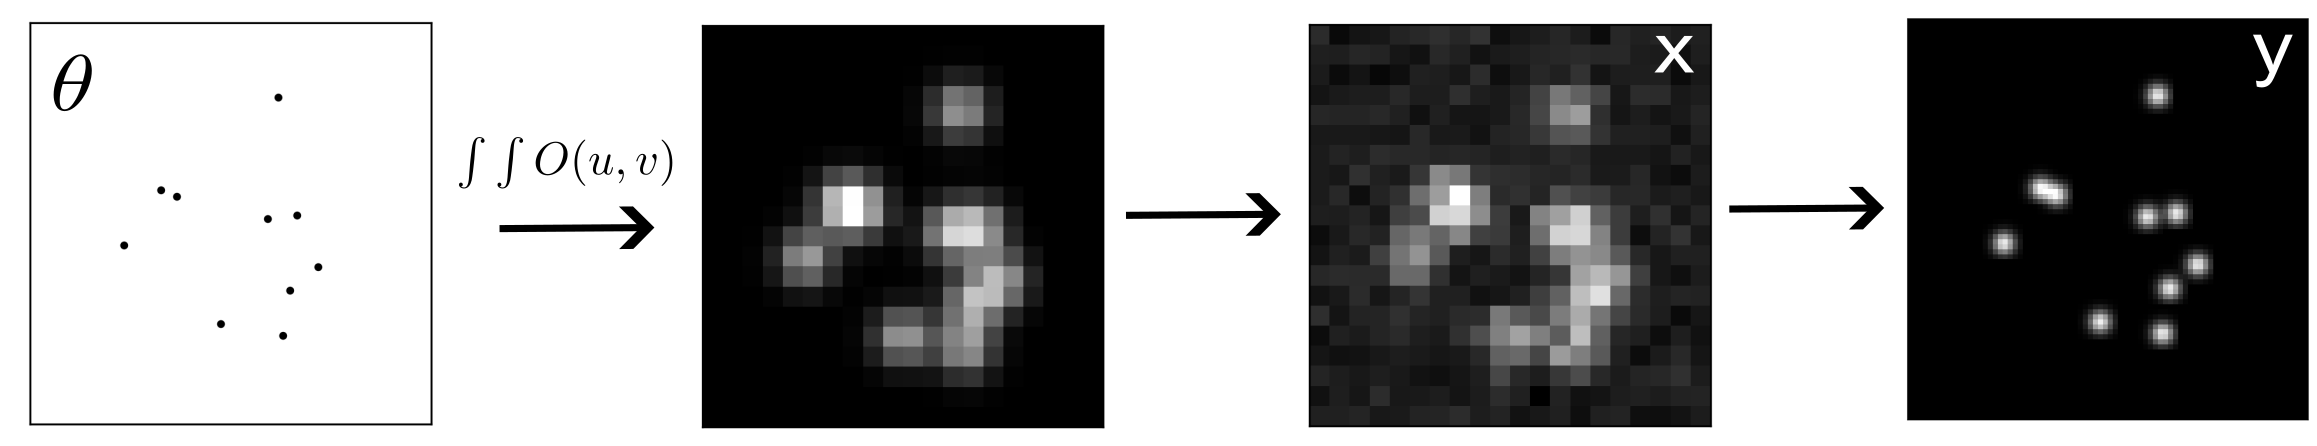
\includegraphics[width=\textwidth]{../../dissertation/dissertation/media/Generation.png}\\

%\begin{itemize}
%\item Would like to estimate a high-resolution $\bold{y}$ from low-resolution $\bold{x}$, but it is many to one
%\item Must then model a \emph{distribution} over $\bold{y}$ i.e., $p_{\theta}(\bold{y}|\bold{x})$
%\end{itemize}
%\end{frame}

%\begin{frame}{Trivial example of sampling from a mixture of Gaussians}
%\begin{textblock*}{13cm}(1.0cm, 1.5cm)
%\animategraphics[width=13cm,autoplay,loop]{30}{../../dissertation/dissertation/media/langevin/langevin-}{1}{152}
%\end{textblock*}
%\begin{textblock*}{13cm}(1.0cm, 6.5cm)
%Consider a two-component Gaussian mixture $p(\bold{x}) = \sum_{k=1}^{2}\pi_{k}\mathcal{N}(\mu_{k},\sigma_{k}^{2})$\\
%\vspace{0.5cm}
%If we know $\nabla\log p(\bold{x})$ we can sample from $p(\bold{x})$ with Langevin dynamics: 
%\begin{equation*}
%\bold{x}_{i} = \bold{x}_{i-1} + \epsilon \nabla\log p(\bold{x}) + \sqrt{2\epsilon}\eta \;\; \eta\sim %\mathcal{N}(0,I)
%\end{equation*}
%\end{textblock*}
%\end{frame}

\setbeamertemplate{footline}{
    \hbox{%
    \begin{beamercolorbox}[wd=\paperwidth,ht=1.0ex,dp=1.5ex,leftskip=2ex,rightskip=2ex]{page ooter}%
        \footnotesize
        \usebeamerfont{title in head/foot}%
        Super-resolution of nucleosome nanodomains \textit{in-vivo} \hfill
            %\insertsection \hfill
        \insertframenumber{} / \inserttotalframenumber
    \end{beamercolorbox}}%
}


\section{Super-resolution of nucleosome nanodomains \textit{in-vivo}}

\subsection{Interaction of transcriptional condensates with nucleosome nanodomains}

\begin{frame}{Hierarchical structure of chromatin}

\begin{textblock*}{10cm}(3.0cm,1.25cm)
\includegraphics[width=10cm]{../../dissertation/dissertation/media/Chromatin}
\\
\vspace{0.4cm}
Fyodorov, D. et al. Nat Rev Mol Cell Biol \textbf{19}, (2018).
\end{textblock*}

\end{frame}

\begin{frame}{Bromodomain protein 4 (BRD4) binds acetylated chromatin}

\includegraphics[width=12cm]{../../dissertation/dissertation/media/Epigenetic}

\begin{textblock*}{10cm}(1.5cm,4.5cm)
Zheng, B. et al. Molecular Cell \textbf{16}, (2023).
\end{textblock*}

\begin{textblock*}{10cm}(1.5cm,8.5cm)
Fillapakoulos, P. et al. Nature \textbf{468}, (2010).
\end{textblock*}

\end{frame}

\setbeamertemplate{footline}{
    \hbox{%
    \begin{beamercolorbox}[wd=\paperwidth,ht=1.0ex,dp=2ex,leftskip=2ex,rightskip=2ex]{page footer}%
        \footnotesize
        \usebeamerfont{title in head/foot}%
        \textbf{Seitz C.} et al. 2024 (In Review) Phys Rev Lett.\hfill
        \insertframenumber{} / \inserttotalframenumber
    \end{beamercolorbox}}%
}


\begin{frame}{BRD4 mutations to probe effects on chromatin structure}

\begin{textblock*}{5cm}(2.0cm,1.75cm)
\includegraphics[width=5cm]{../../dissertation/dissertation/media/TwoColor}
\end{textblock*}

\begin{textblock*}{5cm}(7.75cm,1.25cm)
\includegraphics[width=5cm]{../../brd4/brd4/media/AlphaFoldStructure}
\end{textblock*}

\begin{textblock*}{5cm}(8.25cm,5.0cm)
AlphaFold BRD4 1-1362aa 
\end{textblock*}


\begin{textblock*}{10cm}(2.0cm,7.0cm)
%\includegraphics[width=10cm]{../../brd4/brd4/media/Mutations}
\begin{itemize}
\item 7A mutant - Constitutively unphosphorylated
\item 7D mutant - Constitutively phosphorylated
\item BD mutant - Bromodomain deactivated
\end{itemize}
\end{textblock*}

\end{frame}


\begin{frame}{BRD4 recruitment to nuclesome nanodomains}
\begin{center}
\includegraphics[width=10cm]{../../brd4/brd4/media/Figure-0.png}
\end{center}
\begin{itemize}
\item Phosphorylation enhances BRD4 binding to acetylated chromatin
\item Hyperphosphorylation - resistance mechanism to BD loss (Shu 2016)
\end{itemize}
\end{frame}

\begin{frame}{BRD4 chromatin binding controls chromatin mobility}
\includegraphics[width=13cm]{../../brd4/brd4/media/Figure-3}
\vspace{0.1in}
\begin{itemize}
\item H2B is sparsely labeled for particle tracking 
\item Reduced diffusion coefficient $D$ in BRD4 mutants
\item Increased $D$ in cells exposed to (+)-JQ1
\end{itemize}

\end{frame}


\begin{frame}{BRD4 binding is necessary for maintenance of nucleosome nanodomains}
\begin{textblock*}{10cm}(2.0cm,1.5cm)
\includegraphics[width=10cm]{../../brd4/brd4/media/Figure-2.png}
\end{textblock*}

\begin{textblock*}{13cm}(1.0cm,8.0cm)
\begin{itemize}
\item H2B is densely labeled for super-resolution imaging
\item BRD4 chromatin binding activity controls nanodomain density
\end{itemize}
\end{textblock*}

\end{frame}

\begin{frame}{Coarse grained molecular dynamics of chromatin at 310K}
\begin{textblock*}{10cm}(2.5cm,1.5cm)
\includegraphics[width=10cm]{../../brd4/brd4/media/Rouse}
\end{textblock*}
\begin{textblock*}{13cm}(1.0cm,9.0cm)
\begin{itemize}
\item 100kb chromatin beads connected by harmonic bonds (Rouse model)
\end{itemize}
\end{textblock*}
\end{frame}

\begin{frame}{Coarse grained molecular dynamics of chromatin binders at 310K}
\includegraphics[width=12cm]{../../brd4/brd4/media/MD-1}
Chromatin chains interact with binders via the potential 
\begin{equation*}
U_{ij} = \epsilon \left(1-\left(\frac{|r_{ij}|}{R_{0}}\right)^{2}\right)^{3}
\end{equation*}
\begin{itemize}
\item $A$ ($B$) type particles represent unacetylated (acetylated) chromatin beads
\item BRD4-like $C$ particles bind $B$ type particles with variable energies
\end{itemize}
\end{frame}

\begin{frame}{Multivalent chromatin binding reduces chromatin mobility}
\includegraphics[width=12cm]{../../brd4/brd4/media/MD-2}
Integrate Brownian dynamics: $\dot{r} = \gamma^{-1}\nabla U + \sqrt{2 k_{B}T}\gamma^{-1/2}\xi \;\; \gamma = 10^{-6}$\\
\vspace{1cm}
Stochastic forcing is a delta-correlated noise $\xi \sim \mathcal{N}(0,1), \langle \xi(t)\xi(t+\tau)\rangle = \delta(\tau)$
\end{frame}

\setbeamertemplate{footline}{
    \hbox{%
    \begin{beamercolorbox}[wd=\paperwidth,ht=1.0ex,dp=1.5ex,leftskip=2ex,rightskip=2ex]{page ooter}%
        \footnotesize
        \usebeamerfont{title in head/foot}%
        \insertshorttitle \hfill
            %\insertsection \hfill
        \insertframenumber{} / \inserttotalframenumber
    \end{beamercolorbox}}%
}

\begin{frame}{Summary of contributions}
\begin{itemize}
\item First generative model of super-resolution microscopy images from low-resolution inputs
\item Applied SPAD array for counting fluorescent molecules in widefield microscopy
\item First data supporting control of chromatin architecture by transcriptional condensates
\end{itemize}
\end{frame}

\begin{frame}{Selected Publications}

\begin{itemize}

\item \textbf{C. Seitz}, D. Fu, M. Liu, H. Ma, and J. Liu. \textit{BRD4 phosphorylation regulates the structure of chromatin nanodomains}. In Review. Phys Rev Lett. 2024

\item \textbf{C. Seitz} and J. Liu. \textit{Uncertainty-aware localization microscopy by variational diffusion}. In Progress. 2024

\item \textbf{C. Seitz} and J. Liu. \textit{Quantum enhanced localization microscopy with a single photon avalanche diode array}. In Progress. 2024

\item M. Locatelli\textsuperscript{\textdagger}, J. Lawrimore\textsuperscript{\textdagger}, H. Lin\textsuperscript{\textdagger}, S. Sanaullah, \textbf{C. Seitz}, D. Segall, P. Kefer, S. Moreno Naike, B. Lietz, R. Anderson, J. Holmes, C. Yuan, G. Holzwarth, B. Kerry, J. Liu, K. Bonin, P. Vidi. \textit{DNA damage reduces heterogeneity and coherence of chromatin motions}. PNAS 12 July 2022; 119 (29): 1-11

\item M. Zhang, \textbf{C. Seitz}, G. Chang, F. Iqbal, H. Lin, and J. Liu \textit{A guide for single-particle chromatin tracking in live cell nuclei}. Cell Biology International 15 January 2022; 46 (5): 683-700

\item S. Roy, \textbf{C. Seitz}, M. Samaddar, J. Liu \textit{Bayesian Inference of Transcriptional Kinetics of GBP5 by Single-Molecule Imaging}. In Progress. 2024

\end{itemize}
\end{frame}



\begin{frame}{Acknowledgements}
\begin{textblock*}{16cm}(1.7cm,1.5cm)
\includegraphics[width=16cm]{../../dissertation/dissertation/media/Lab.png}
\end{textblock*}

\begin{textblock*}{14cm}(1.7cm,8.5cm)
Thank you!
\end{textblock*}

\end{frame}



\end{document}